%% LyX 2.3.1-1 created this file.  For more info, see http://www.lyx.org/.
%% Do not edit unless you really know what you are doing.
\documentclass[notheorems, preprint, mathpazo]{jeea}
\usepackage[T1]{fontenc}
\usepackage{color}
\usepackage{verbatim}
\usepackage{url}
\usepackage{amsmath}
\usepackage{amsthm}
\usepackage{amssymb}
\usepackage{graphicx}
\usepackage[authoryear]{natbib}
\makeatletter

%%%%%%%%%%%%%%%%%%%%%%%%%%%%%% LyX specific LaTeX commands.
\newcommand{\noun}[1]{\textsc{#1}}

%%%%%%%%%%%%%%%%%%%%%%%%%%%%%% Textclass specific LaTeX commands.
\newenvironment{lyxlist}[1]
	{\begin{list}{}
		{\settowidth{\labelwidth}{#1}
		 \setlength{\leftmargin}{\labelwidth}
		 \addtolength{\leftmargin}{\labelsep}
		 \renewcommand{\makelabel}[1]{##1\hfil}}}
	{\end{list}}
\theoremstyle{definition}
\newtheorem*{defn*}{\protect\definitionname}
\theoremstyle{plain}
\newtheorem{lem}{\protect\lemmaname}
\theoremstyle{plain}
\newtheorem{prop}{\protect\propositionname}

%%%%%%%%%%%%%%%%%%%%%%%%%%%%%% User specified LaTeX commands.

%\usepackage{enumerate}
\renewcommand{\theenumi}{\roman{enumi}}
\usepackage{graphicx}
\usepackage[export]{adjustbox}
\DeclareGraphicsExtensions{.pdf,.jpeg,.png,.eps}
\usepackage{enumitem}
\usepackage{changepage}


\usepackage{booktabs}
\newcommand{\specialcell}[2][c]{%
  \begin{tabular}[#1]{@{}c@{}}#2\end{tabular}}

\newcounter{parentnumber}
\usepackage{multirow}
\allowdisplaybreaks

\usepackage{amsmath}
\newtheorem{result}{Result}
\usepackage{bbm}

\newtheoremstyle{boldremark}
    {\dimexpr\topsep/2\relax} % space above
    {\dimexpr\topsep/2\relax} % space below
    {}          % body font
    {}          % indent amount
    {\bfseries} % theorem head font
    {.}         % punctuation after theorem head
    {.5em}      % space after theorem head
    {}          % theorem hed spec. (empty = "normal")

\theoremstyle{boldremark}
\newtheorem{brem}{Remark} % remarks are numbered within sections

\makeatother

\usepackage{babel}
\providecommand{\definitionname}{Definition}
\providecommand{\lemmaname}{Lemma}
\providecommand{\propositionname}{Proposition}

\begin{document}
\title{Can Trade Taxes be a Major Source of Government Revenue?}
\Author{Ahmad}{Lashkaripour}{Indiana University}{alashkar@indiana.edu}

\Abstract{The tariff-for-revenue argument has been invoked repeatedly in recent
	years to justify protectionism. It is motivated by the belief that
	a country with market power can use trade taxes to raise revenue from
	foreign consumers and producers. This paper develops a new sufficient
	statistics methodology to evaluate this claim for a wide range of
	countries. I show that $(a)$ even large countries have limited market
	power. $(b)$ So, before retaliation by trading partners, the average
	country can \emph{beneficially} replace only 16\% of its domestic
	tax revenues with trade taxes. $(c)$ After retaliation, however,
	50\% of the collected trade tax revenues disappear, governments are
	forced to increase domestic taxes to counter their shrinking tax base,
	and real GDP drops across-the-board by an average of 7\%. On the flip
	side, these findings indicate $(d)$ the gains from multilateral trade
	agreements are also 30\% larger once we account for the fiscal cost
	of trade wars.}

\maketitle

\section{Introduction}

Recently, the president of the United States praised tariffs as a
\emph{\textquotedblleft great revenue producer.\textquotedblright }
This remark has resurfaced old debates that are reminiscent of ``the
Great Tariff Debate of 1888.''\footnote{See, for example, \url{https://beta.washingtonpost.com/politics/2019/07/16/tariff-revenue-trump-tweets-things-you-need-know/}}
At the core of these ongoing debates lie a set of unresolved questions:
\begin{lyxlist}{00.00.0000}
	\item [{$(a)$}] Absent the threat of retaliation, can a country possibly
	gain from replacing domestic tax revenues with trade tax revenues?
	\item [{$(b)$}] If so, what fraction of government spending can be financed
	with only trade taxes?
	\item [{$(c)$}] Above all, how large are the potential losses from retaliation?
\end{lyxlist}
To answer questions $(a)$ and $(b)$ we need to compute the excess
burden of trade taxation and determine what fraction of the burden
is borne by foreign consumers and producers. The traditional literature
on this issue simplifies this task by assuming that countries are
small and possess \emph{no} export or import market power.\footnote{See \citet{anderson1996trade} for a review of the literature on trade
	tax reform in the presence of revenue considerations.} Under this assumption, the burden of trade taxation falls entirely
on the tax-imposing economy, and by \citeauthor{diamond1971optimal}'s
\citeyearpar{diamond1971optimal} \emph{production efficiency principle,}
trade taxes become strictly less efficient than other revenue-raising
tax instruments even for a non-cooperative country.

For all its merits, the traditional approach contradicts the recent
assertion by \citet{alvarez2007general} that even small economies
possess export/import market power after we account for national technology
differentiation and general equilibrium linkages. In such cases, a
non-cooperative country can gain \emph{unilaterally} from replacing
a fraction of its domestic taxes with equal-yield trade taxes. We
have virtually no evidence, though, as to what fraction of the domestic
tax revenue can be replaced with trade taxes in these circumstances.

Answering question $(c)$ is even more complicated, as it requires
knowledge of Nash revenue-raising trade taxes that will prevail under
multilateral retaliation. Calculating these taxes involves simultaneously
solving for the optimal tax response of many countries while taking
into account a wide range of general equilibrium interdependencies.
Performing such a procedure can be infeasible with standard quantitative
techniques unless we limit our analysis to a small sample of countries
and industries.

To overcome these challenges, I derive \emph{sufficient statistics}
formulas for revenue-maximizing trade taxes in a multi-industry general
equilibrium trade model that admits both product/technology
differentiation, and an endogenous supply of labor. Mapping these
formulas to data allows me to calculate the effectiveness of trade
taxes at raising revenue \emph{before} and \emph{after} retaliation
for a wide range of countries and across many industries.

My analysis finds that $(a)$ the degree of technology differentiation
is low-enough that even large countries possess limited market power.
$(b)$ So, even before retaliation by trading partners, the average
country can \emph{beneficially} replace only 16\% of its domestic
tax revenues with trade tax revenues. $(c)$ After retaliation, however,
50\% of the collected trade tax revenues disappear. The domestic tax
base also shrinks after retaliation, prompting governments to increase
domestic taxes. More importantly, all parties lose from these developments
and real GDP drops by more than 7\% globally. On the flip side, these
findings suggest that $(d)$ the gains from multilateral trade agreements
are 30\% larger once we account for the fiscal cost of trade wars.

Section \ref{sec:Theoretical-Model} presents the baseline theoretical
model, which is a multi-industry, multi-country \citet{Eaton2002}
model with endogenous labor supply. All countries possess export and
import market power, the degree of which depends on country size and
the industry-level trade elasticities. All countries also have access
to a complete set of revenue-raising tax instruments, including trade
taxes as well as domestic income and VAT taxes. I also analyze several
extensions to the baseline model to account for $(i)$ pre-existing
domestic market distortions, $(ii)$ industry-specific factors of
production, $(iii$) within-country worker heterogeneity, and $(iv)$
input-output linkages.

Section \ref{subsec: Replacing-Income-tax} analyzes a tax reform,
whereby a non-cooperative government replaces domestic taxes with
equal-yield trade taxes in order to maximize the contribution of trade
tax revenues to its budget. I consider two distinct cases, where trade
tax revenues are maximized $(a)$ irrespective of their effect on
aggregate welfare, and $(b)$ subject to not worsening aggregate welfare.
I am particularly interested in Case $(b)$, which determines the
maximum share of domestic tax revenues that can be \emph{beneficially}
replaced with trade taxes.

I analytically solve the government's problem in both cases, deriving
sufficient statistics formulas for revenue-maximizing export and import
taxes. These formulas indicate that, regardless of the underlying
model parameters, import taxes can \emph{beneficially} replace a small
fraction of the domestic tax revenue. To elaborate, import taxes are
more effective at raising revenue when trade elasticities are low.
But in that case, the import tax is also borne primarily by domestic
consumers. This trade-off between effectiveness and efficiency means
that even a non-cooperative government can \emph{beneficially} replace
a modest fraction of its domestic tax revenues with import taxes.
Export taxes, however, do \emph{not} face a similar trade-off and can be more-or-less
effective depending on the underlying model parameters.

Section \ref{subsec:Effectiveness-Under-Retaliation} analyzes the
consequences of retaliation by trading partners. Retaliation, expectedly,
leads to a reduction in trade tax revenues and inflicts a welfare
loss on all parties. My analysis, however, highlights two welfare
cost channels that have received little attention in the prior literature.
First, in the trade war that ensues after retaliation,
labor supply decisions become distorted due to an increase in consumer
prices. Second, the domestic tax base shrinks, prompting governments
to raise domestic taxes to maintain real public spending. The latter
channel corresponds to the fiscal cost of a trade war.

My analysis of multilateral retaliation yields another basic insight:
The consequences of retaliation are greater in circumstances where
trade taxes are a more appealing fiscal instrument for non-cooperative
governments. The intuition behind this result is that when trade elasticities
are low, governments can capitalize on their higher national market
power and raise a greater amount of trade tax revenues. But under
these circumstances, countries are also more dependent on foreign
trade, making them more vulnerable to retaliation.

Section \ref{subsec: Mapping-the-Sufficient} demonstrates how the
sufficient statistics tax formulas, derived in Section \ref{subsec: Replacing-Income-tax},
can be mapped to data. Doing so measures the effectiveness of trade
taxes at raising revenue based on a simple procedure that requires
knowledge of only $(i)$ industry-level trade elasticities, $(ii)$
the labor supply elasticity, and $(iii)$ observable trade shares.
It also determines the welfare and fiscal consequences of multilateral
retaliation by trading partners.

The procedure outlined in Section \ref{subsec: Mapping-the-Sufficient}
plays a pivotal role in my quantitative analysis, especially in the
case of multilateral retaliation. This new procedure determines the
consequences of retaliation in one simple step, by solving a system
of non-linear equations. In comparison, the traditional approach to
analyzing multilateral retaliation involves an iterative procedure,
where each iteration performs many constrained numerical optimizations.
Unlike the new approach, the standard approach can become infeasible
unless we restrict attention to a small set of countries and industries.

Section \ref{sec:Quantitative-Implementation} estimates the industry-level
trade elasticities using industry-level trade data from the World
Input-Output Database (WIOD) and tariff data from UNCTAD-TRAINS. Together,
these data-sets cover 43 major economies plus an aggregate of the
rest of the world and span 56 traded and service-related industries.
Using the estimated elasticities and the procedure outlined in Section
\ref{subsec: Mapping-the-Sufficient}, I produce four basic results:
\begin{enumerate}
	\item Before retaliation, trade taxes can \emph{beneficially} replace only
	16\% of the domestic tax revenue for the average country. This outcome
	reflects the fact that industry-level trade elasticities are relatively
	low and even large countries possess limited market power.
	\item After retaliation, trade tax revenues decline by 50\%. The domestic
	tax base also shrinks by 3\%, prompting governments to raise domestic
	taxes to maintain real public spending. Real aggregate income also
	drops in all countries by around 7\% on average. Altogether, after
	retaliation, every \$1 million of domestic tax revenue that is replaced
	with trade tax revenue imposes an excess burden of \$2.5 million on
	the economy.\footnote{The efficiency loss associated with trade taxes can reduce if we account
		for the lower monitoring and enforcement cost associated with these
		taxes (see \citet{emran2005selective}, \citet{besley2013taxation},
		and \citet{best2015production}).} 
	\item In countries where trade taxes are relatively more effective at raising
	revenue, they\emph{ }are also less efficient (i.e., they inflict a
	greater excess burden on the economy). This finding is related to
	the aforementioned trade-off between the effectiveness and efficiency
	of revenue-raising trade taxes. The trade-off is driven by the fact
	that when countries are net importers of low-trade elasticity goods,
	their import taxes are more effective at raising revenue. But such
	countries are also more reliant on trade and are more exposed to the
	negative consequences of retaliation. 
	\item The gains from trade agreements are 30\% larger, once we account for
	$(a)$ the fiscal cost of trade wars, and $(b)$ distortions to labor
	supply decisions. The gains from multilateral trade agreements can
	be measured on the basis that they avert the losses from multilateral
	trade wars. I simply find that the cost of multilateral trade wars
	are larger than previously estimated, once we account for cost channels
	$(a)$ and $(b)$.
\end{enumerate}

\subsection*{Related Literature}

The debate regarding the \emph{potential} size of trade tax revenues
has advanced little since ``the Great Tariff Debate of 1888.'' This
paper is, to my knowledge, the first to formally measure the effectiveness
of trade taxes at replacing domestic tax revenues. \citet{irwin1998higher}
who investigates whether the US economy was positioned to the right
or left of the tariff Laffer curve circa 1888 is perhaps the most
similar paper to mine in this regard.

Previously, \citet{baunsgaard2010tax} and \citet{cage2018tax} have
highlighted the fiscal cost of tariff liberalization using historical
data. The present paper contributes to these studies by highlighting
the fiscal cost of a multilateral trade war. I argue that trade wars
inflict so much inefficiency on the global economy that they shrink
the domestic tax base in most countries. Governments involved in a
tariff war must, therefore, increase domestic taxes to maintain public
spending.

This paper also contributes to an old and mature literature that studies
the fiscal aspects of trade tax reforms (e.g., \citet{keen2002coordinating,keen2005coordinating,emran2005selective,anderson2016sufficient}).\footnote{The above literature builds on earlier analyses of piecemeal tariff
reforms, e.g., \citet{hatta1977theory} and \citet{fukushima1979tariff},
which abstracted from the fiscal cost channel} This literature typically assumes that countries possess no export
or import market power, which automatically rules out any unilateral
gains from trade taxation---see \citet{dixit1985tax} for a comprehensive
review.\footnote{\citet{dixit1985tax} shows that, even when countries have market
power, trade taxes should be combined with domestic taxes to reach
the non-cooperative first-best outcome. If countries lack market power,
though, the first-best can be reached with only zero trade taxes.
This latter claim derives from the \citet{diamond1971optimal}\emph{
production efficiency principle.}} The present paper, in comparison, estimates the degree of export
and import market power for various countries. Guided by these estimates,
I then present an alternative argument against taxing-trade-for-revenue,
which emphasizes $(a)$ the ineffectiveness of trade taxes at raising
revenue, and $(ii)$ the high cost of retaliation.

There is an even older argument against taxing trade for revenue or
other purposes, which dates back to \citet{baldwin1982inefficacy}.
It states that governments are prone to miscalculating the impacts
of their policies. As a result, they adopt policy choices that are
from optimal and even detrimental to own's welfare. Analyses of the
recent US-China trade war confirm this old argument (e.g., \citet{amiti2019cep};
\citet{fajgelbaum2019return}; \citet{waugh2019consumption}; \citet{handley2020rising}).\footnote{The aforementioned studies show that the recent tariffs on China worsened
the terms-of-trade and aggregate welfare in the US economy, even without
full retaliation by the Chinese government. One way to interpret these
findings is that the US government applied tariffs that were far from
their \emph{unilaterally} optimal rate, to begin with.}

On the theory side, my two-tier approach for characterizing the revenue-maximizing
trade tax schedule shares commonalities with \citet{costinot2015comparative}
and \citet{costinot2016micro}. The former split the optimal trade
policy problem into an inner and outer problem. This procedure simplifies
the characterization of unilaterally optimal trade taxes in a Ricardian
model. The latter splits the optimal policy problem into a micro-problem
and a macro-problem. This approach provides a transparent characterization
of the unilaterally optimal trade taxes under firm-level heterogeneity
and selection effects.

On a broader level, this paper contributes to a recent literature
that quantifies the gains from regional and multilateral trade agreements
(e.g., \citet{ossa2014trade,ossa2016quantitative}; \citet{caliendo2014estimates};
\citet{bagwell2018quantitative}). The existing literature often assumes
that labor is inelastically supplied in each country. Under this assumption,
the elimination of trade agreements has no fiscal cost or does not
distort labor supply decisions. I argue that accounting for these
previously-overlooked cost channels can magnify the gains from trade
agreements.

\section{\label{sec:Theoretical-Model}Theoretical Model}

\paragraph*{Environment.}

The world economy consists of $i=1,...,N$ countries, with $\mathbb{C}$
denoting the set of countries. Labor is the sole factor of production.
Country $i$ is populated by $L_{i}$ individuals, each endowed with
one unit of labor. All individuals are perfectly mobile across the
production of different goods but are immobile across countries; and
are paid a country-specific wage, $w_{i}$. There are $k=1,...,K$
industries, with $\mathbb{K}$ denoting the set of industries, each
of which can differ in fundamentals such as the trade elasticity.

\paragraph*{Preferences. }

There is a continuum of homogeneous goods indexed by $\omega\in\Omega_{k}\equiv[0,1]$
in industry $k$. The utility of the representative consumer in country
$i$ who consumes basket $\boldsymbol{q}$ and supplies $L$ units
of labor are described by the following function
\[
U_{i}(\boldsymbol{q},L)=\mathcal{Q}_{i}(\boldsymbol{q})-v(L).
\]
In the above formulation, $v(L)=L^{1+\frac{1}{\kappa}}/\left(1+\frac{1}{\kappa}\right)$
accounts for disutility from labor, ensuring the elasticity of labor
supply is constant. Preferences for final goods are given by the
following Cobb-Douglas-CES utility aggregator
\[
\mathcal{Q}_{i}(\boldsymbol{q})=\prod_{k=1}^{K}\left(\int_{\omega\in\Omega_{k}}q(\omega)^{\rho_{k}}d\omega\right)^{\frac{e_{i,k}}{\rho_{k}}},
\]
where $\rho_{k}\in(0,1)$, while $e_{i,k}$ denotes the constant share
of expenditure on industry $k$ ($\sum_{k=1}^{K}e_{i,k}=1$). 

\paragraph*{Production.}

Labor is the only factor of production and markets are perfectly competitive.
The marginal cost of producing good $\omega$ in country $j$ and
delivering to market $i$ is given by
\[
c_{ji,k}(\omega)=\tau_{ji,k}w_{j}/z_{j,k}(\omega),
\]
where productivity, $z_{j,k}(\omega)$, is independently drawn from
a Fr\'echet distribution, $F_{j,k}(z)=\exp(-T_{j,k}z^{-\theta_{k}})$.
$\tau_{ji,k}\geq1$ denotes the iceberg trade cost associated with
exporting from country $j$ to market $i$, with $\tau_{ii,k}=1$
for all $i\in\mathbb{C}$.\footnote{I also assume that $\tau_{ji,k}\geq\tau_{j\ell,k}\tau_{\ell i,k}$
for all $j$, $i$, and $\ell\in\mathbb{C}$.} Considering the above cost function, country $j$ can supply good
$\omega$ to market $i$ at a perfectly competitive price, $p_{ji,k}(\omega)=c_{ji,k}(\omega)$. 

\paragraph*{Trade and Income Taxes.}

Country $i$ has access to a full set of $(a)$ industry-level import
taxes, $\{t_{ji,k}\},$ that are applied to all goods imported from
origin $j\neq i$; as well as $(b)$ industry-level export taxes,
$\{x_{ij,k}\}$, that are applied to goods exported to destination
$j\neq i$. By construction, $x_{ii,k}=t_{ii,k}\equiv0$ for all $k$.
Trade taxes create a wedge between the producer price, $p_{ji,k}(\omega)$,
and the consumer price, $\tilde{p}_{ji,k}(\omega)$ of every traded
variety. In particular,
\[
\tilde{p}_{ji,k}(\omega)=(1+x_{ji,k})(1+t_{ji,k})p_{ji,k}(\omega),\ \ \ \forall\omega\in\Omega_{k}.
\]
Given the constancy of the unit labor cost, the \emph{direct} passthrough
of taxes on to consumer prices (i.e., the passthrough net of general
equilibrium wage effects) is complete. This feature is consistent
with recent findings in \citet{amiti2019impact} and \citet{fajgelbaum2019return}.
In Appendix \ref{sec:Accounting-for-Passthrough}, however, I relax
the constant-unit-labor-cost assumption and discuss how this amendment
affects the main results of the paper.

Each country $i$ also has access to a \emph{linear} income tax, $\delta_{i}$,
which raises a revenue $\delta_{i}w_{i}L_{i}$. Both trade and income
taxes have distortionary effects on the economy. The trade taxes directly
distort consumer prices, whereas the income tax decreases the labor
supply.\footnote{To be specific, $L_{i}=\left([1-\delta_{i}]w_{i}/\tilde{P}_{i}\right)^{\kappa}$
where $\tilde{P}_{i}$ is the price index associated with $Q_{i}$. } Importantly, as is well-known from the public finance literature,
a linear income tax is equivalent to a uniform consumption (or VAT)
tax. So, we can henceforth view $\delta$ as an instrument that accounts
for the collective sum of flat income and consumption taxes.

\paragraph*{General Equilibrium.}

Consumers in Market $i$ purchase variety $\omega$ from the cheapest
supplier. So, the actual price paid for good $\omega$ satisfies
\[
\tilde{p}_{i,k}(\omega)=\min_{j\in\mathbb{C}}\left\{ \tilde{p}_{ji,k}(\omega)\right\} .
\]
Following the steps in \citet{Eaton2002}, the share of country $i$'s
expenditure on goods originating from country $j$ is given by
\[
\lambda_{ji,k}(\boldsymbol{t},\boldsymbol{x};\boldsymbol{w})=\frac{T_{j,k}\left[(1+t_{ji,k})(1+x_{ji,k})\tau_{ji,k}w_{j}\right]^{-\theta_{k}}}{\sum_{\ell\in\mathbb{C}}T_{\ell,k}\left[(1+t_{\ell i,k})(1+x_{\ell i,k})\tau_{\ell i,k}w_{\ell}\right]^{-\theta_{k}}},
\]
where $\boldsymbol{w}\equiv\{w_{i}\}$. Market $i$'s total expenditure
on country $j$ goods is, therefore, given by $X_{ji,k}(\boldsymbol{w})=\lambda_{ji,k}(\boldsymbol{w})e_{i,k}Y_{i}$,
with $Y_{i}$ denoting total expenditure in Country $i$. The national-level
budget constraint (BC) requires that total expenditure in country
$i$ is the sum of personal expenditure from \emph{net} wage income,
$(1-\delta_{i})w_{i}L_{i}$ and government expenditure form tax revenues,
$G_{i}\equiv\delta_{i}w_{i}L_{i}+\mathcal{R}_{i}$:
\begin{equation}
[\textrm{BC}]\ \ \ \ \ \ \ \ \ \ Y_{i}=w_{i}L_{i}(\boldsymbol{t},\boldsymbol{x},\boldsymbol{\delta};\boldsymbol{w})+\mathcal{R}_{i}(\boldsymbol{t},\boldsymbol{x},\boldsymbol{\delta};\boldsymbol{w},\boldsymbol{Y}).\label{eq: Eq Income}
\end{equation}
In the above expression, $\boldsymbol{Y}\equiv\{Y_{i}\}$; while $L_{i}(.)=([1-\delta_{i}]w_{i}/\tilde{P}_{i})^{\kappa}$
where $\tilde{P}_{i}$ is the price index of the aggregate consumption
basket.\footnote{To be specific, the consumer price index is given by $\tilde{P}_{i}=\tilde{e}_{i}\prod_{k}\tilde{P}_{i,k}^{e_{i,k}}$,
where $\tilde{e}_{i}=\prod_{k}e_{i,k}^{-e_{i,k}}$ and $\tilde{P}_{i,k}=\Gamma\left(\frac{\theta_{k}-1/\rho_{k}}{\theta_{k}}\right)^{-\rho_{k}}\left[\sum_{j=1}^{N}T_{j,k}\left[(1+t_{ji,k})(1+x_{ji,k})\tau_{ji,k}w_{j}\right]^{-\theta_{k}}\right]^{-1/\theta_{k}}$,
with $\Gamma(.)$ denoting the Gamma function.}$\mathcal{R}_{i}(.)$ denotes the portion of government spending that
is financed by trade tax revenues, and is equal to
\small{\begin{equation}
\hspace{-0.1in}\mathcal{R}_{i}(\boldsymbol{t},\boldsymbol{x},\boldsymbol{\delta};\boldsymbol{w},\boldsymbol{Y})\equiv\sum_{j=1}^{N}\sum_{k=1}^{K}\left[\frac{t_{ji,k}}{1+t_{ji,k}}\lambda_{ji,k}(\boldsymbol{t},\boldsymbol{x};\boldsymbol{w})e_{i,k}Y_{i}+\frac{x_{ij,k}}{(1+x_{ij,k})(1+t_{ij,k})}\lambda_{ij,k}(\boldsymbol{t},\boldsymbol{x};\boldsymbol{w})e_{j,k}Y_{j}\right].\label{eq: Tax Revenue}
\end{equation}}
Equation \ref{eq: Eq Income} along with the representative consumer's
budget constraint, ensure that trade is balanced between countries.
For any vector of taxes, $\boldsymbol{x}\equiv\{x_{ji,k}\}$, $\boldsymbol{t}\equiv\{t_{ji,k}\}$,
and $\boldsymbol{\delta}\equiv\{\delta_{i}\}$, equilibrium wages,
$\boldsymbol{w}$, and expenditure levels, $\boldsymbol{Y}$, should
satisfy Equation \ref{eq: Eq Income} and the labor market clearing
condition:
\begin{equation}
[\textrm{LMC}]\ \ \ \ \ \ \ \ \ \ w_{i}L_{i}=\sum_{j=1}^{N}\sum_{k=1}^{K}\left[\frac{1}{(1+t_{ij,k})(1+x_{ij,k})}\lambda_{ij,k}(\boldsymbol{t},\boldsymbol{x};\boldsymbol{w})e_{j,k}Y_{j}\right].\label{eq: Eq Wage}
\end{equation}
Considering this, all equilibrium outcomes can be uniquely determined
given the \emph{policy$\times$wage$\times$income} combination $(\boldsymbol{t},\boldsymbol{x},\boldsymbol{\delta};\boldsymbol{w},\boldsymbol{Y})$.
The following definition outlines this point.
\begin{defn*}
\emph{The policy$\times$wage$\times$income combination $(\boldsymbol{t},\boldsymbol{x},\boldsymbol{\delta};\boldsymbol{w},\boldsymbol{Y})$
is feasible if given taxes $(\boldsymbol{t},\boldsymbol{x},\boldsymbol{\delta})$,
equilibrium vectors $\boldsymbol{w}$ and $\boldsymbol{Y}$ satisfy
Equations \ref{eq: Eq Income} and \ref{eq: Eq Wage}. Relatedly,
$\mathbb{F}$ denotes the set of all feasible policy$\times$wage$\times$income
combinations.}
\end{defn*}
To be clear, in the above definition, $\boldsymbol{w}$ and $\boldsymbol{Y}$
are implicit functions of the tax schedule $(\boldsymbol{t},\boldsymbol{x},\boldsymbol{\delta})$.
So, the effect of a tax change on different equilibrium outcomes can
always be decomposed into a direct effect and a general equilibrium
effect that operates through a change in $\boldsymbol{w}$ and $\boldsymbol{Y}$.

\section{\label{subsec: Replacing-Income-tax}Effectiveness of Trade Taxes
at Raising Revenue}

As discussed earlier, a country that possesses market power can beneficially
replace a \emph{portion} of their income tax revenue with trade tax
revenues. The adoption of trade taxes, though, worsens the welfare
of one's trading partners as they bear part of the trade tax burden.
Moreover, if trading partners retaliate, all possible gains from unilateral
trade taxation disappear. Considering these points, I first analyze
the effectiveness of revenue-raising trade taxes before retaliation.
I subsequently analyze the consequences of multilateral retaliation.

\subsection{Effectiveness Before Retaliation }

Suppose a government is neither cooperative nor is it concerned by
retaliation. Such a government may be tempted to use trade taxes for
revenue-generation, but faces two basic questions:
\begin{enumerate}
\item What share of the government's budget can be financed with trade taxes
if social welfare was not a binding consideration?
\item What share of the government's budget can be financed with trade taxes
without worsening domestic social welfare?
\end{enumerate}
Question 1 is relevant to governments that have a strict political
or institutional preference for trade taxation (i.e., \textbf{\emph{Case 1}}).
The government's objective, in this case, is to maximize the contribution
of trade tax revenues to its budget irrespective of how social welfare
is affected---see \citet{bhagwati1988protectionism}. This scenario
is especially relevant to the current political climate wherein multiple
governments have turned to trade tax revenues to fund political redistribution
in their country, even though these policies have compromised social
welfare.\footnote{One prominent example concerns the Trump administration's farm subsidies,
which were financed with import tariff hikes. See \citet{fajgelbaum2019return}
for the consequences of these tariff hikes on social welfare in the
US economy. }

Question 2, on the other hand, is relevant to governments who attach
a prominent weight to social welfare in their objective function (i.e.,
\textbf{\emph{Case 2}}). Such a government is willing to replace
income taxes with equal-yield trade taxes insofar as domestic social
welfare does not deteriorate in the process. There is ample evidence
that some governments exhibit this type of attitude towards trade
policy. \citeauthor{goldberg1999protection}'s \citeyearpar{goldberg1999protection}
analysis of the U.S.'s trade policy indicates that the U.S. government
attached a prominent weight to social welfare (over political economy
motives) circa 1983. Below, I analyze Cases 1 and 2 separately, elaborating
more on their implicit differences throughout.

\subsubsection*{Case 1: Strict Political Preference for Trade Taxation. }

To answer questions $(i)$, I need to determine the \emph{revenue-maximizing}
trade tax schedule in each country $i$. That is the trade tax schedule
that maximizes the contribution of trade tax revenues to government
$i$'s expenditure, given applied taxes in the rest of the world.
These taxes solve the following problem:
\begin{align*}
\max_{(\boldsymbol{t},\boldsymbol{x},\boldsymbol{\delta};\boldsymbol{w},\boldsymbol{Y})\in\mathbb{F}}\  & \mathcal{R}_{i}\left(\boldsymbol{t}_{i},\boldsymbol{x}_{i};\boldsymbol{t}_{-i},\boldsymbol{x}_{-i},\boldsymbol{\delta};\boldsymbol{w},\boldsymbol{Y}\right)\ \ \ \ (\textrm{P1})\\
s.t. & \ \ \delta_{i}w_{i}L_{i}+\mathcal{R}_{i}(.)=\overline{G}_{i},
\end{align*}
where $\boldsymbol{t}_{-i}\equiv\{t_{j\iota,k}\}_{\iota\neq i}$ and
$\boldsymbol{x}_{-i}\equiv\{x_{\iota j,k}\}_{\iota\neq i}$ denote
the vector of applied taxes in the rest of the world. $\overline{G}_{i}$
denotes total government spending under the status quo. The \emph{revenue-neutrality}
constraint in (P1), therefore, ensures that total government spending
or total tax revenue is preserved under the new tax schedule. Note
that we can replace this constraint with one that asserts the perseverance
of \emph{real} government spending, $\overline{G}_{i}/\tilde{P}_{i}$.
With this choice of constraint, however, the optimal tax formulas
will remain the same up-to a uniform tax shifter---I formally solve
this alternative problem in Appendix \ref{sec: Real Revenue Neut.}
and highlight its subtle differences throughout this section.

Problem (P1) is plagued with various general equilibrium interdependencies.
However, as discussed below, we can still analytically solve (P1)
and derive \emph{sufficient statistics} formulas for $\boldsymbol{t}_{i}^{*}(.)$
and $\boldsymbol{x}_{i}^{*}(.)$. An important step in this process
is to invoke the multiplicity of revenue-maximizing taxes and break
Problem (P1) into two sub-problems. The presence of multiplicity is
outlined by the following lemma.
\begin{lem}
For any $a\in\mathbb{R}_{+}$ $(i)$ if $\textrm{A}\equiv(\boldsymbol{1}+\boldsymbol{t}_{i},\boldsymbol{t}_{-i}$,$\boldsymbol{1}+\boldsymbol{x}_{i},\boldsymbol{x}_{-i},\boldsymbol{\delta};w_{i},\boldsymbol{w}_{-i})\in\mathbb{F}$,
then $\textrm{A}'\equiv(a(\boldsymbol{1}+\boldsymbol{t}_{i}),\boldsymbol{t}_{-i},(\boldsymbol{1}+\boldsymbol{x}_{i})/a,\boldsymbol{x}_{-i},\boldsymbol{\delta};aw_{i},\boldsymbol{w}_{-i})\in\mathbb{F}$;
moreover, $(ii)$ the share of trade tax revenue-to-income tax revenue
is preserved under allocations $\textrm{A}$ and $\textrm{A}'$ :
$\mathcal{R}_{i}(\textrm{A})/\delta_{i}w_{i}L_{i}=\mathcal{R}_{i}(\textrm{A}')/\delta_{i}w'_{i}L'_{i}$.\footnote{To economize on the notation, Lemma 1 is cast in terms of feasible
tax-wages combinations, $\textrm{A}\equiv(\boldsymbol{1}+\boldsymbol{t},\boldsymbol{1}+\boldsymbol{x},\boldsymbol{\delta};\boldsymbol{w})$.
The lemma can be equivalently expressed in terms of feasible tax-wage-income
combinations, $\textrm{\ensuremath{\tilde{A}}}\equiv(\boldsymbol{1}+\boldsymbol{t},\boldsymbol{1}+\boldsymbol{x},\boldsymbol{\delta};\boldsymbol{w},\boldsymbol{Y})$.}
\end{lem}
The above lemma, which is proven in Appendix \ref{sec:Proof-of-Lemma},
is akin to the celebrated Lerner symmetry. It states that an across-the-board
shift in country $i$'s import taxes, export taxes, and wage rate
will multiply the total revenue in nominal terms, but will preserve
the share of trade tax revenue in total tax revenue. The Lerner symmetry
states that such a transformation will also preserve welfare.

Considering Lemma 1, we can split Problem (P1) into two sub-problems.\textcolor{red}{}\footnote{Splitting the optimal tax problem into an upper- and lower-tier problem
is reminiscent of the two-tier approach adopted by \citet{costinot2015comparative}
and \citet{costinot2016micro}. The former splits the optimal trade
policy problem into an inner problem that takes the relative wage
as given and an outer problem that determines the optimal relative
wage. The latter splits the optimal policy problem into a micro-problem
that determines the firm-level wedges that deliver aggregate quantities
at the lowest cost and a macro-problem that determines the optimal
aggregate quantities.} First, a lower-tier problem that maximizes $\mathcal{R}_{i}(.)$
subject to total government revenue adding up to an arbitrary value
$G$. This step determines the optimal tax rates up-to a constant
tax shifter. Second, an upper-tier problem chooses the constant tax
shifter in order to satisfy the revenue-preserving constraint $G=\overline{G}_{i}$.
Even after splitting Problem P1 as noted, deriving an analytical solution
is complicated by general equilibrium interrelations. But as shown
in Appendix \ref{sec: Proof-of-Proposition 1}, this task can be accomplished
by appealing to Lemma 1, envelope conditions, and some basic results
from consumer theory. 
\begin{prop}
\label{prop: revenue-maximizing P1} The trade tax rates that maximize
country $i$'s revenue from trade taxes (for a fixed level of government
spending $G$) are given by the following formulas
\begin{align*}
1+t_{ji,k}^{*}=\left[1+\frac{1}{\theta_{k}\lambda_{ii,k}^{*}}\right](1+\bar{t}_{i}),\ \ \ \ \ \ \ \ \  & \ \ \ \forall j\neq i;\ \forall k\in\mathbb{K}\\
1+x_{ij,k}^{*}=\left[1+\frac{1}{\theta_{k}(1-\lambda_{ij,k}^{*})}\right](1+\bar{t}_{i})^{-1}, & \ \ \ \ \ \forall j\neq i;\ \forall k\in\mathbb{K},
\end{align*}
where $\bar{t}_{i}\in\mathbb{R}_{+}$ is a tax shifter that regulates
the nominal tax revenue and is chosen to satisfy the revenue-preserving
constraint.\footnote{The superscript ``$*$'' indicates that the expenditure shares are
evaluated in the equilibrium that occurs under the revenue-maximizing
tax rates. }
\end{prop}
Following Lemma 1, the country-specific tax shifter, $\bar{t}_{i}$,
is pinned down by the revenue-preserving constraint in Problem ($\textrm{P1}$),
i.e., the upper-tier problem. More specifically, if the government
in country $i$ raises trade taxes according to the formulas specified
by Proposition \ref{prop: revenue-maximizing P1}, then there is a
unique $\bar{t}_{i}$ that ensures total tax revenue remains equal
to $\bar{G}_{i}$. To deal with the multiplicity of tax solutions,
Theorem 1 implicitly assumes that $\delta_{i}$ is normalized to its
pre-reform value. As shown in Appendix \ref{sec: Real Revenue Neut.},
under the alternative specification where (P1) is solved subject to
\emph{real }revenue-neutrality, $\bar{t}_{i}$ can be normalized to
zero without loss of generality but $\delta_{i}$ should be chosen
to satisfy the real revenue-neutrality constraint.

The key advantage of Proposition \ref{prop: revenue-maximizing P1}
is that it characterizes the revenue-maximizing trade tax schedule
as a function of two \emph{sufficient statics}:\emph{ $(a)$}industry-level
trade elasticities, and $(b)$ observable expenditure shares. As we
will see in Section \ref{subsec: Mapping-the-Sufficient}, this feature
allows us to solve the entire vector of revenue-maximizing trade taxes
(before and after retaliation) in one simple step as a function of
estimable elasticities and observables. 

We can appeal to the Laffer curve to gain more intuition about the
tax formulas presented under Proposition \ref{prop: revenue-maximizing P1}.
When solving Problem (P1), the tax authority in country $i$ faces
a basic trade-off: On one hand, increasing the trade tax rate has
a positive \emph{arithmetic} effect on tax revenues. On the other
hand, increasing trade taxes has a negative \emph{economic} effect
on tax revenues, as it limits foreign trade and shrinks the trade
tax base. In light of this trade-off, trade tax revenues are maximized
at the peak of the Laffer curve where the export and import tax rates
are proportional to the inverse the demand elasticity facing national-level
exports and imports. 

As such, the \emph{revenue-maximizing} trade taxes characterized by
Proposition \ref{prop: revenue-maximizing P1} are distinct from \emph{optimal}
-welfare-maximizing- trade taxes unless the trade elasticities are
uniform across industries.\footnote{See \citet{costinot2015comparative} and \citet{beshkar2020cost}
for a characterization of optimal trade taxes in general equilibrium,
multi-industry settings. } If trade elasticities exhibit great heterogeneity across industries,
the tax rates specified by Theorem 1 can actually worsen real income
in the tax-imposing. With this background, I next characterize the
tax rates that maximize the trade tax revenue without worsening real
income in the tax-imposing country. 

\subsubsection*{Case 2: No Political Preference for Trade Taxation. }

Now consider a government that is non-cooperative but has no strict
political or institutional preference for trade taxation either. Such
a government is willing to finance government spending with trade
taxes, but to the extent that social welfare is not deteriorated.
As noted earlier, evidence from existing policy practices suggest
that some governments do indeed attach a prominent weight to social
welfare (\citet{goldberg1999protection}). To determine the effectiveness
of trade taxes for such a government, we need to solve the following
problem that includes an additional constraint imposing welfare-neutrality:
\begin{align*}
\max_{(\boldsymbol{t},\boldsymbol{x},\boldsymbol{\delta};\boldsymbol{w},\boldsymbol{Y})\in\mathbb{F}}\  & \mathcal{R}_{i}\left(\boldsymbol{t}_{i},\boldsymbol{x}_{i};\boldsymbol{t}_{-i},\boldsymbol{x}_{-i},\boldsymbol{\delta};\boldsymbol{w},\boldsymbol{Y}\right)\ \ \ \ (\textrm{P2})\\
s.t. & \ \ \delta_{i}w_{i}L_{i}+\mathcal{R}_{i}(.)=\overline{G}_{i},\\
 & \ \ \Delta W_{i}(\boldsymbol{t}_{i},\boldsymbol{x}_{i};\boldsymbol{t}_{-i},\boldsymbol{x}_{-i},\boldsymbol{\delta};\boldsymbol{w},\boldsymbol{Y})\geq0.
\end{align*}
The above problem differs from Problem (P1) in a key aspect: Given
the additional constraint, $\Delta W_{i}(.)\ge0$, Problem (P2) determines
the extent to which a government can \emph{beneficially} replace domestic
income taxes with trade taxes. To elucidate this distinction, recall
that the welfare-maximizing and revenue-maximizing trade tax schedules
do not necessarily coincide. Specifically, to maximize trade tax revenues,
the government has to distort domestic prices in a way that can be
detrimental to domestic social welfare. The welfare-neutrality constraint
added to Problem (P2) accounts for the tendency of certain governments
to avoid such a situation.

If trade elasticities are sufficiently low and homogeneous, then the
revenue-maximizing trade tax schedule is welfare improving by design.
That is, 
\[
\Delta W_{i}(\boldsymbol{t}_{i}^{*},\boldsymbol{x}_{i}^{*};\boldsymbol{t}_{-i},\boldsymbol{x}_{-i},\boldsymbol{\delta};\boldsymbol{w},\boldsymbol{Y})>0
\]
where $\boldsymbol{t}_{i}^{*}$ and $\boldsymbol{x}_{i}^{*}$ are
the revenue-maximizing tax rates specified by Proposition \ref{prop: revenue-maximizing P1}.
In that case, Problems (P1) and (P2) are identical. However, if trade
elasticities are too high and governments possess limited market power,
the revenue-maximizing trade taxes specified by Proposition \ref{prop: revenue-maximizing P1}
can worsen welfare, i.e., $\Delta W_{i}(\boldsymbol{t}_{i}^{*},\boldsymbol{x}_{i}^{*};...)<0$.
In that case, it is impossible to derive exact analytic formulas for
trade taxes that solve P2. However, we can analytically solve P2 to
a first-order approximation by appealing to the following lemma.
\begin{lem}
$\Delta W_{i}(\boldsymbol{t}'_{i},\boldsymbol{x}'_{i};\boldsymbol{t}_{-i},\boldsymbol{x}_{-i},\boldsymbol{\delta};\boldsymbol{w},\boldsymbol{Y})>0$
if $\boldsymbol{t}'_{i}=\boldsymbol{0}$ and $\boldsymbol{x}'_{i}=\left\{ 1/\theta_{k}(1-\lambda_{ij,k})\right\} _{j,k}$.
\end{lem}
The above lemma states that any country $i$ can improve its welfare
by imposing zero tariffs and the revenue-maximizing export tax schedule.
The above lemma strictly generalizes the assertion in \citet{alvarez2007general}
to an economy that accommodates many asymmetric industries. It states
that, in the presence of technology differentiation, even a small
country can gain unilaterally from trade taxation. These unilateral
gains, though, worsen \emph{global} efficiency and impose a burden
on other countries.

Let $\boldsymbol{t}_{i}^{*}$ and $\boldsymbol{x}_{i}^{*}$ denote
the solution to (P2). Lemma 2 establishes that $1+x_{ij,k}^{*}=\left[1+1/\theta_{k}(1-\lambda_{ij,k})\right](1+\bar{t}_{i})^{-1}$,
where $\bar{t}_{i}$ is chosen to satisfy the revenue-neutrality constraint.
Moreover, since $W_{i}(.)$ is a concave function of tariffs, it trivially
follows that $(1+\bar{t}_{i})(1+1/\theta_{k}\lambda_{ii,k})\geq1+t_{ji,k}^{*}\geq1+\bar{t}_{i}$.
Hence, given that both $\mathcal{R}_{i}(.)$ and $W_{i}(.)$ are concave
in $\boldsymbol{t}_{i}$, we can approximate the solution to (P2)
based on the solution to (P1), as noted by the following proposition.
\begin{prop}
\label{prop: revnenue-maximizing P2}The trade tax rates that maximize
country $i$'s trade tax revenues without deteriorating domestic welfare
are given by
\begin{align*}
1+t_{ji,k}^{*}\approx\left[\bar{\alpha}_{i}+\left(1+\frac{1}{\theta_{k}\lambda_{ii,k}^{*}}\right)(1-\bar{\alpha}_{i})\right](1+\bar{t}_{i}), & \ \ \ \forall j\neq i;\ \forall k\in\mathbb{K}\\
1+x_{ij,k}^{*}=\left(1+\frac{1}{\theta_{k}\left(1-\lambda_{ij,k}^{*}\right)}\right)(1+\bar{t}_{i})^{-1}, & \ \ \ \forall j\neq i;\ \forall k\in\mathbb{K},
\end{align*}
where $\bar{t}_{i}\in\mathbb{R}_{+}$ is a tax shifter that regulates
the nominal tax revenue and is chosen to satisfy the revenue-neutrality
constraint and $\bar{\alpha}_{i}\in(0,1)$ is a uniform tax shifter
that is chosen to satisfy the welfare-neutral constraint, $\Delta W_{i}(.)=0$. 
\end{prop}
The gain more intuition about the above proposition, note two extreme
cases. If $\bar{\alpha}_{i}=0$, the above import tax rate maximizes
trade tax revenue while possibly worsening welfare. alternatively,
if $\bar{\alpha}_{i}=1$, the above import tax rate is strictly welfare
improving based on Lemma 2. So, by increasing $\alpha_{i}$ from an
initial value of zero, we can eventually detect an import tax rate
close to the revenue-maximizing rate that satisfies the welfare-neutrality
constraint.

The difference between the tax schedules implied by Problems (P1)
and (P2) is regulated by $(i)$ the level of, and $(ii)$ the cross-industry
heterogeneity in trade elasticities. If trade elasticities are low,
then countries possess significant export market power. In that case,
the large gains from export taxation assure that the solutions to
(P1) and (P2) coincide. Likewise, if trade elasticities are rather
uniform across industries, revenue-raising import taxes are less detrimental
to domestic welfare. In that case, the welfare-neutrality constraint
is less likely to be binding and the solutions to (P1) and (P2) will
once again coincide.

On the contrary, if industry-level trade elasticities are low and
high-heterogeneous, then the tax schedule that solves (P2) yields
a strictly smaller revenue. On one hand, when trade elasticities are
heterogeneous, the revenue-maximizing import taxes are borne primarily
by domestic consumers. On the other hand, as $\theta_{k}\rightarrow\infty$,
export taxes are also borne primarily by domestic firms. The following
remark summarizes these arguments.\vspace{0.1in}

\begin{brem}

\emph{If industry-level trade elasticities are high, ``export''
taxes are an ineffective non-cooperative fiscal instrument, because
they are borne primarily by the tax-imposing economy. Similarly, if
trade elasticities are highly heterogeneous across industries, ``import''
taxes are an ineffective fiscal instrument. Because increasing the
amount of import tax revenue, in that case, coincides with increasing
the incidence of taxation on domestic consumers.}\end{brem} \vspace{0.1in}

In light of the above remark, a credible assessment of revenue-raising
trade taxes requires credible estimates for trade elasticities. A
formal estimation of the trade elasticities is performed later in
Section \ref{sec:Quantitative-Implementation}. Before that, however,
I discuss the consequences of retaliation and also how to map the
sufficient statistics tax formulas to data.

\subsection{\label{subsec:Effectiveness-Under-Retaliation}Effectiveness Under
Retaliation}

If historical records are any indication, a country that turns to
trade taxation will face retaliation from the rest of the world. I
henceforth mode retaliation as a scenario where non-cooperative countries
simultaneously erect revenue-maximizing trade taxes.\footnote{Alternatively, we can assume that countries erect welfare-maximizing
trade taxes. Under that assumption, the best export tax response will
remain identical. However, the best import tax response will consist
of less-heterogeneous import taxes. See \citet{lashkaripour2019measuring}
for an analysis of multilateral retaliation under welfare-maximizing
import taxes.} To determine the best tax response for each country in this scenario,
we need to solve (P1) simultaneously for all $N$ countries. To elaborate,
let $\boldsymbol{t}_{i}^{*}(\boldsymbol{t}_{-i},\boldsymbol{x})$
and $\boldsymbol{x}_{i}^{*}(\boldsymbol{t},\boldsymbol{x}_{-i})$
denote the solutions to (P1) for country $i$. The full vector of
revenue-maximizing taxes is the solution to the following system:
\[
\begin{cases}
\boldsymbol{t}_{1}=\boldsymbol{t}_{1}^{*}(\boldsymbol{t}_{-1},\boldsymbol{x});\ \ \  & \boldsymbol{x}_{1}=\boldsymbol{x}_{1}^{*}(\boldsymbol{t},\boldsymbol{x}_{-1})\\
\vdots & \vdots\\
\boldsymbol{t}_{N}=\boldsymbol{t}_{N}^{*}(\boldsymbol{t}_{-N},\boldsymbol{x});\ \ \  & \boldsymbol{x}_{N}=\boldsymbol{x}_{N}^{*}(\boldsymbol{t},\boldsymbol{x}_{-N})
\end{cases}.
\]
Before moving forward, I should emphasize that the above problem is
plagued with the curse of dimensionality when confronted with standard
optimization techniques. To make this point clear, let me outline
the standard technique used by \citet{ossa2014trade} and others to
approach these kinds of problems. The researcher starts with an initial
guess for revenue-maximizing taxes, namely, $\boldsymbol{t}_{0}^{*}$
and $\boldsymbol{x}_{0}^{*}$. Then, they update $\boldsymbol{t}_{i}^{*}$
and $\boldsymbol{x}_{i}^{*}$, given $\boldsymbol{t}_{0}^{*}$ and
$\boldsymbol{x}_{0}^{*}$, for each country $i$. This second step
requires solving $N$ constrained global optimizations, each involving
$2\left(N-1\right)K$ tax rates and $2N$ equilibrium outcomes (namely,
$\boldsymbol{w}$ and $\boldsymbol{Y}$). After updating the initial
guess, the same procedure is repeated iteratively until convergence
is achieved.\footnote{\citet{perroni2000new} and \citet{ossa2014trade} apply this iterative
method to compute Nash tariffs in the event of a tariff war. As noted
by \citet{ossa2016quantitative}, the efficiency of the standard iterative
optimization technique can be enhanced by $(i)$ parallelizing the
country-specific optimizations, and $(ii)$ providing analytic derivatives
for the objective function.} With many countries and industries, this approach can become infeasible
to implement.

To overcome the curse of dimensionality, I can appeal to the \emph{sufficient
statistics} formulas specified by Theorem \ref{prop: revenue-maximizing P1}.
This is possible because Theorem \ref{prop: revenue-maximizing P1}
characterizes the best tax response of any country $i$, given applied
taxes by other countries. Simultaneously solving the system of best
tax response functions, yields the tax rates that will prevail under
retaliation.
\begin{prop}
\label{prop: Nash}In the event of retaliation by trading partners,
the Nash revenue-maximizing trade taxes can be solved as a solution
to the following system
\begin{align*}
\begin{cases}
1+t_{ji,k}^{*}=\left(1+\frac{1}{\theta_{k}\lambda_{ii,k}(\boldsymbol{t}^{*},\boldsymbol{x}^{*})}\right)(1+\bar{t}_{i}) & \ \ \ \forall j\neq i;\ \forall k\\
1+x_{ij,k}^{*}=\left(1+\frac{1}{\theta_{k}\left[1-\lambda_{ij,k}(\boldsymbol{t}^{*},\boldsymbol{x}^{*})\right]}\right)(1+\bar{t}_{i})^{-1}, & \ \ \ \forall j\neq i;\ \forall k
\end{cases},
\end{align*}
where $\boldsymbol{t}^{*}$ and $\boldsymbol{x}^{*}$ denote the vector
of Nash trade taxes all over the world, while $\bar{t}_{i}$ is a
country-specific tax shifter that is pinned down by the revenue-neutrality
constraint.
\end{prop}
It is needless to say that after retaliation, all the possible benefits
from unilateral trade taxation disappear. All countries lose due to
trade reduction and trade tax revenues decline due to a shrinking
of the trade tax base. The extent to which countries lose is a function
of the industry-level trade elasticities: On one hand, when trade
elasticities are low, retaliatory tariffs are higher. On the other
hand, when trade elasticities are low, trade reduction is also more
detrimental to welfare. The following remark summarizes these arguments.\vspace{0.1in}

\begin{brem}

\emph{When industry-level trade elasticities are low, $(a)$ trade
taxes are a more effective (non-cooperative) revenue-raising instrument;
but $(b)$ the potential losses from retaliation are also larger.}\end{brem} \vspace{0.1in}

The system specified by Proposition \ref{prop: Nash} solves for Nash
trade taxes that maximize revenue. Following my earlier discussion,
this scenario is more appropriate if governments have a political
or institutional preference for trade taxation. Alternatively, retaliation
can occur in the form of governments adopting welfare-maximizing Nash
taxes. In that case, we can adopt a fairly similar approach to compute
the Nash tariffs---see \citet{lashkaripour2019measuring} for a thorough
discussion on the determination of welfare-maximizing Nash tariffs.
Remark 2, however, can be stated as is under either scenario.\footnote{When Nash trade taxes are chosen to maximize welfare, export taxes are given by the same formula. That is, they strictly increase with
the industry-level trade elasticity. So, with lower trade elasticities, a trade war both shrinks
global trade more intensively and inflicts a greater welfare loss on involved countries. } 

Importantly, the consequences of retaliation depend on whether government
revenues are maintained in \emph{real} or \emph{nominal} terms. In
the former case, retaliation has an additional fiscal cost, which
operates by shrinking the income tax base. That is, when the income
tax base shrinks, governments are obliged to raise $\delta_{i}$ to
maintain real government expenditure. Doing so imposes an additional
cost on the economy by distorting labor supply decisions---see Appendix
\ref{sec: Real Revenue Neut.} for a formal analysis. In comparison,
to maintain nominal expenditure, the government can simply adjust
the uniform tax shifter $\bar{t}_{i}$, which is welfare neutral per
Lemma 1.

\section{\label{subsec: Mapping-the-Sufficient}Mapping Sufficient Statistics
Formulas to Data}

In this section, I demonstrate how the \emph{sufficient statistics}
formulas derived in Section \ref{subsec: Replacing-Income-tax} can
be mapped to data. Doing so $(a)$ quantifies the extent to which
trade taxes can replace existing income tax revenues, and $(b)$ determines
the welfare consequences of trade tax adoption \emph{before} and \emph{after}
retaliation. As argued earlier, performing tasks $(a)$ and $(b)$
can be infeasible with standard quantitative techniques, especially
in the case of retaliation. 

In the interest of space, I focus my discussion around the more complex
case where countries retaliate against each other. I subsequently
outline how similar results apply to the simpler, pre-retaliation
case. To present my argument, I adopt the conventional exact hat-algebra
notation, where $\hat{z}\equiv z^{*}/z$ denotes the change in a generic
variable $z$ when moving from the factual equilibrium to the counterfactual
Nash equilibrium. The basic idea here is to invoke the hat-algebra
notation and express the revenue-maximizing tax formulas specified
by Proposition \ref{prop: Nash} in changes. Specifically, noting
that $\lambda_{ii,k}^{*}=\lambda_{ii,k}\hat{\lambda}_{ii,k}$ and
$\lambda_{ij,k}^{*}=\lambda_{ij,k}\hat{\lambda}_{ij,k}$, the revenue-maximizing
Nash import and export taxes can be formulated in changes as follows:
\[
1+t_{ji,k}^{*}=\left[1+\frac{1}{\theta_{k}\lambda_{ii,k}\hat{\lambda}_{ii,k}}\right](1+\bar{t}_{i});\ \ \ \ \ \ \ \ \ \ \ \ \ \ \ \ 1+x_{ij,k}^{*}=\left[1+\frac{1}{\theta_{k}(1-\lambda_{ij,k}\hat{\lambda}_{ij,k})}\right](1+\bar{t}_{i})^{-1}
\]
Using the same logic, we can express the equilibrium conditions specified
by Equations \ref{eq: Eq Income} and \ref{eq: Eq Wage} in changes.
We can then simultaneously solve the revenue-maximizing tax formulas
alongside the equilibrium conditions to compute the change in key
economic variables when moving from the status quo to the Nash equilibrium.
The following Proposition formally outlines this procedure.
\begin{prop}
\label{prop: hat-algebra}The Nash revenue-maximizing trade taxes,
$\{t_{ji,k}^{*}\}$ and $\{x_{ij,k}^{*}\}$, as well as their effect
on wages, $\{\hat{w}_{i}\}$, total income, $\{\hat{Y}_{i}\}$, and
labor supply, $\{\hat{L}_{i}\}$, can be solved as a solution to the
following system of equations:
\[\hspace*{-0.1in}
\begin{cases}
1+t_{ji,k}^{*}=\left[1+\frac{1}{\theta_{k}\hat{\lambda}_{ii,k}\lambda_{ii,k}}\right](1+\bar{t}_{i});\ \ \ \ \ \ \ \ \ \ \ 1+x_{ij,k}^{*}=\left[1+\frac{1}{\theta_{k}\left(1-\hat{\lambda}_{ij,k}\lambda_{ij,k}\right)}\right](1+\bar{t}_{i})^{-1}\\
\hat{\lambda}_{ji,k}=\left[\frac{(1+x_{ji,k}^{*})(1+t_{ji,k}^{*})}{(1+x_{ji,k})(1+t_{ji,k})}\hat{w}_{j}\right]^{-\theta_{k}}\hat{\tilde{P}}_{i,k}^{\theta_{k}};\ \ \ \ \ \ \  \hat{\tilde{P}}_{i,k}=\sum_{\ell}\left(\left[\frac{(1+x_{\ell i,k}^{*})(1+t_{\ell i,k}^{*})}{(1+x_{\ell i,k})(1+t_{\ell i,k})}\hat{w}_{\ell}\right]^{-\theta_{k}}\lambda_{\ell i,k}\right)^{-\frac{1}{\theta_{k}}}\\{}
[\textrm{BC}]\ \ \ \ \hat{Y}_{i}Y_{i}=\hat{w}_{i}\hat{L}_{i}w_{i}L_{i}+\hat{\mathcal{R}}_{i}\mathcal{R}_{i};\ \ \ \ \ \ \ \ \ \ \ \ \ \ \ \ \ \hat{L}_{i}=\left[\hat{w}_{i}/\prod\hat{\tilde{P}}_{i,k}^{e_{i,k}}\right]^{\kappa}\\{}
[\textrm{LMC}]\ \ \ \ \hat{w}_{i}\hat{L}_{i}w_{i}L_{i}=\sum_{k}\sum_{j}\left[\frac{1}{(1+t_{ij,k}^{*})(1+x_{ij,k}^{*})}\hat{\lambda}_{ij,k}\lambda_{ij,k}e_{j,k}\hat{Y}_{j}Y_{j}\right]\\
\hat{\mathcal{R}}_{i}\mathcal{R}_{i}=\sum_{k}\sum_{j\neq i}\left(\frac{t_{ji,k}^{*}}{1+t_{ji,k}^{*}}\hat{\lambda}_{ji,k}\lambda_{ji,k}e_{i,k}\hat{Y}_{i}Y_{i}+\frac{x_{ij,k}^{*}}{(1+t_{ij,k}^{*})(1+x_{ij,k}^{*})}\hat{\lambda}_{ij,k}\lambda_{ij,k}e_{j,k}\hat{Y}_{j}Y_{j}\right)\\
\hat{\mathcal{R}}_{i}\mathcal{R}_{i}+\delta_{i}\hat{w}_{i}\hat{L}_{i}w_{i}L_{i}=\mathcal{R}_{i}+\delta_{i}w_{i}L_{i}
\end{cases}.
\]
Moreover, solving the above system requires knowledge of only structural
elasticities, $\{\theta_{k}\}$ and $\kappa$, and observables: namely,
$(i)$ applied taxes, $t_{ji,k}$, $x_{ij,k}$, and $\delta_{i}$;
$(ii)$ expenditure shares, $\lambda_{ji,k}$ and $e_{i,k}$; and
$(iii)$ national expenditure and output, $Y_{i}$ and $w_{i}L_{i}$.
\end{prop}
The system specified by Proposition \ref{prop: hat-algebra} involves
$3N+NK+N(N-1)K$ independent equations and unknowns---namely, $NK$
import tax rates, $\{t_{i,k}^{*}\}$; $N(N-1)K$ export tax rates,
$\{x_{ij,k}^{*}\}$; $N$ wage changes, $\{\hat{w}_{i}\}$; $N$ labor
supply changes, $\{\hat{L}_{i}\}$; and $N$ income changes, $\{\hat{Y}_{i}\}$.
Solving this system requires knowledge of only $(i)$ observables
($t_{ji,k}$, $x_{ji,k}$, $\delta_{i}$, $\lambda_{ji,k}$, $e_{i,k}$,
$w_{i}L_{i}$, $Y_{i}$), and $(ii)$ estimable elasticities ($\theta_{k}$
and $\kappa$).\footnote{Note that, following Equation \ref{eq: Eq Wage}, $w_{i}L_{i}$ is
implicitly implied by data on $t_{ji,k}$, $x_{ji,k}$, $\lambda_{ji,k}$,
$e_{i,k}$, and $Y_{i}$.} Proposition \ref{prop: hat-algebra}, therefore eliminates the need
to estimate the policy-invariant parameters, $T_{i,k}$, and $\tau_{ji,k}$.
It also rids us of the need to perform an iterative global optimization
procedure. These two simplifications are significant from a quantitative
perspective. Without the aid of Proposition \ref{prop: hat-algebra},
solving for $\boldsymbol{t}^{*}$ and $\boldsymbol{x}^{*}$ would
be effectively infeasible unless we impose strong limits on the number
of countries and industries.

When interpreting Proposition \ref{prop: hat-algebra} one should
take note of a key subtlety. In the counterfactual exercise specified
by Proposition \ref{prop: hat-algebra}, the nominal income tax rate,
$\delta_{i}$, is constant, but the effective income tax rate is declining.
To elaborate, moving from $\textrm{A}\equiv(\bar{\boldsymbol{t}},\boldsymbol{\bar{x}},\boldsymbol{\delta};\boldsymbol{w},\boldsymbol{Y})$
to $\textrm{A}^{'}\equiv(\boldsymbol{t}^{*},\boldsymbol{x}^{*},\boldsymbol{\delta};\boldsymbol{w}',\boldsymbol{Y}')$,
a smaller fraction of the consumer's \emph{real} wage income is being
withdrawn by the income tax. Simply, because a bigger share of the
government's \emph{real} spending is being financed by trade taxes.
In other words, following Lemma 1, Proposition \ref{prop: hat-algebra}
can be reformulated such that $\bar{t}_{i}$ is normalized to zero
and $\hat{\delta}_{i}=\delta_{i}'/\delta_{i}$ is instead treated
as a free-moving variable. Relatedly, Appendix \ref{sec: Real Revenue Neut.}
presents a variant of Proposition \ref{prop: hat-algebra} where $\hat{\delta}_{i}$
is chosen to satisfy \emph{real} revenue-neutrality, which as argued
earlier, has its distinct implications. 

Solving the system specified by Proposition \ref{prop: hat-algebra}
serves two main purposes. First, it determines how the effectiveness
of trade taxes at raising revenue is affected by retaliation. Second,
the system also determines how trade taxation for revenue purposes
ultimately affects welfare, $W_{i}=U_{i}(.)$. The welfare effects
can be calculated using the change in real tax revenue and the real
wage, both of which are implied by Proposition \ref{prop: hat-algebra}. 
\begin{prop}
The welfare consequences of substituting income tax revenue with trade
tax revenue are given by
\[
\hat{W}_{i}=\phi_{i}\frac{\hat{Y}_{i}}{\hat{\tilde{P}}_{i}}+(1-\phi_{i})\frac{\hat{w}_{i}\hat{L}_{i}}{\hat{\tilde{P}}_{i}},
\]
where $\hat{Y}_{i}$, $\hat{w}_{i}\hat{L}_{i}$, and $\hat{\tilde{P}}_{i}=\prod_{k}\left(\hat{\tilde{P}}_{i,k}^{e_{i,k}}\right)$
are implied by the system specified under Proposition \ref{prop: hat-algebra},
while $\phi_{i}\equiv Y_{i}/(Y_{i}-\frac{\kappa}{1+\kappa}(1-\delta_{i})w_{i}L_{i})$
is observable. 
\end{prop}
The proof of the above proposition follows trivially from the fact
that the optimal labor supply in country $i$ is given by $L_{i}=\left([1-\delta_{i}]w_{i}/\tilde{P}_{i}\right)^{\kappa}$.
To put a dollar value on welfare consequences, we can further compute
the excess burden of the tax policy change using the output of Proposition
\ref{prop: hat-algebra}. This step is formally outlined in Appendix
\ref{sec: Excess Burden}.

Finally, we can produce an analog of Proposition \ref{prop: hat-algebra}
to determine the effectiveness of trade taxes for country $i$ before
retaliation. In that case, we need to solve the same system while
setting $x_{nj,k}^{*}=x_{nj,k}$ and $t_{jn,k}^{*}=t_{jn,k}$for all
$n\neq i$. To determine what fraction of the government's expenditure
can be \emph{beneficially} financed with trade taxes, we also need
to replace the optimal import tax formula with that specified by Proposition
\ref{prop: revnenue-maximizing P2}. The tax shifter, $\bar{\alpha}_{i}$,
is then pinned down by introducing an additional equation that imposes
welfare neutrality, i.e., $\hat{W}_{i}=1$.

\subsection{Basic Extensions}

Before moving forward, let me discuss how the results presented earlier
extend to richer environments that admit $(i)$ pre-existing market
distortions, $(ii)$ a variable unit labor cost, and $(iii)$ within-country
income heterogeneity. In the interest of space, I resort to a verbal
discussion of these extensions in the main text. In the appendix,
however, I formally derive analogs for Proposition \ref{prop: hat-algebra}
in these richer environments.

\subsubsection*{Accounting for Pre-Existing Market Distortions.}

My baseline analysis relied on a perfectly competitive model in which
the market equilibrium is efficient. This setup overlooks a possibly
relevant consideration: that using trade taxes to raise revenue may
exacerbate pre-existing market distortions. In Appendix \ref{sec: Accounting-for-Distortions},
I introduce markup distortions into my baseline model. In this alternative
setup, I re-derive \emph{sufficient statistics} formulas for revenue-maximizing
trade taxes and present an analog for Proposition \ref{prop: hat-algebra}.
Doing so indicates that the fraction of income tax revenue that is
replaceable with trade tax revenue remains approximately the same.
However, the deadweight burden associated with revenue-raising trade
taxes is higher if the industry-level markup is negatively correlated
with the industry-level trade elasticity. 

As in the baseline model, we can map sufficient statistics tax formulas
to data to quantify the fiscal properties of trade taxes under markup
distortions. As before, the basic idea is to jointly solve for the
revenue-maximizing tax rates and equilibrium conditions in changes.
As detailed in Appendix \ref{sec: Accounting-for-Distortions}, the
formulas governing the revenue-maximizing tax rates are similar to
those specified under Proposition \ref{prop: hat-algebra}. But the
labor market clearing condition and the budget constraint need to
be revised to account for profits. Specifically, letting $\mu_{k}\geq1$
denote the constant markup associated with industry $k$, the labor
market clearing condition (LMC) and national-level budget constraint
(BC) can be formulated in changes as
\begin{align*}
[\textrm{LMC}]\ \ \ \ \ \ \ \ \ \ \  & \hat{w}_{i}\hat{L}_{i}w_{i}L_{i}=\sum_{k}\sum_{j}\left[\frac{1}{\mu_{k}(1+t_{ij,k}^{*})(1+x_{ij,k}^{*})}\hat{\lambda}_{ij,k}\lambda_{ij,k}e_{j,k}\hat{Y}_{j}Y_{j}\right]\\{}
[\textrm{BC}]\ \ \ \ \ \ \ \ \ \ \ \hat{Y}_{i} & Y_{i}=\hat{w}_{i}\hat{L}_{i}w_{i}L_{i}+\hat{\mathcal{R}}_{i}\mathcal{R}_{i}+\sum_{k}\sum_{j}\left[\frac{\mu_{k}-1}{\mu_{k}(1+t_{ij,k}^{*})(1+x_{ij,k}^{*})}\hat{\lambda}_{ij,k}\lambda_{ij,k}e_{j,k}\hat{Y}_{j}Y_{j}\right].
\end{align*}
The last term in country $i$'s budget constraint corresponds to total
profits collected by firms in that country. This term was zero in
the baseline model, where $\mu_{k}=1$ for all $k$ by assumption.
A basic complication here is that evaluating the above equations requires
information on industry-level markups, which are difficult to recover
from macro-level trade data.

\subsubsection*{Accounting for a Variable Unit Labor Cost.}

The baseline EK model assumes a constant unit labor cost. This assumption
implies that the \emph{direct} passthrough of trade taxes onto consumer
prices is complete once we net out general equilibrium wage effects.
As noted earlier, this assumption is consistent with the findings
in \citet{amiti2019impact} and \citet{fajgelbaum2019return}. In
Appendix \ref{sec:Accounting-for-Passthrough}, however, I derive
\emph{sufficient statistics} formulas for revenue-maximizing trade
taxes in a setup where the unit labor cost is increasing in industry-level
output. Using these formulas, I present an analog for Proposition
\ref{prop: hat-algebra} in the presence of a variable unit labor
cost. This exercise indicates that the revenue-maximizing import (export)
tax rate and the revenue they deliver will be relatively higher (lower)
under an increasing unit labor cost,. However, revenue-maximizing
import (export) taxes will also inflict a greater (smaller) deadweight
loss on the economy.

\subsubsection*{Accounting for Within-Country Income Heterogeneity.}

The results presented above hold without qualification if we all allow
for an exogenous distribution of abilities across workers---an assumption
that is commonplace in the public finance literature. In Appendix
\ref{sec: Worker Heterogeneity}, however, I look beyond this special
case by presenting an extension of the model featuring multiple types
of workers as in \citet{galle2017slicing}. Worker types are heterogeneous
in their abilities, and sort into industries accordingly \`a la Roy.
Solving Problem ($\textrm{P1}$) in this setup indicates that using
trade taxes for revenue generation can worsen income inequality if
high-income workers have a comparative advantage in high-$\theta$
industries. Considering this, the baseline model (which accounts for
only representative welfare effects) may understate the cost of revenue-raising
trade taxes.

\subsubsection*{Accounting for Input-Output Linkages.}

Following \citet{caliendo2014estimates}, we can introduce input-output
linkages into the baseline EK model. Under this extension, which is
formally presented in Appendix \ref{sec: Input-Output Linkages},
the elasticity of import demand is moderated by the input-output structure.
Specifically, a tax on import good $ji,k$ will raise the price of
domestic goods that use $ji,k$ as an input. The inflated price of
domestic goods will, in turn, moderate the tax-induced reduction in
import demand. As a result, the revenue-maximizing import tax rate
will be relatively higher than the baseline rate. By comparison, the
revenue-maximizing export tax rate is given by the same formula specified
under Proposition \ref{prop: revenue-maximizing P1}, provided that
each country is sufficiently small relative to the rest of the world--see
Appendix \ref{sec: Input-Output Linkages} for specific details. 

In addition to influencing the revenue-maximizing trade tax rate,
input-output linkages create ripple effects that magnify the fiscal
and welfare burden associate with every dollar of tax revenue. Specifically,
the trade-impeding effects of trade taxes can multiply through the
input-output network, leading to a greater-than-baseline shrinkage
in global trade for the same tax rate. As such, the welfare consequences
of retaliation will be more drastic after we account for input-output
linkages. Relatedly, the shrinkage of the trade tax base will be more
pronounced after retaliation, implying a lower revenue for the same
tax rate. As detailed in Appendix \ref{sec: Input-Output Linkages},
these welfare and fiscal consequences can be quantified using a similar
approach to that presented under Proposition \ref{prop: hat-algebra}. 

\section{\label{sec:Quantitative-Implementation}Quantitative Implementation}

The section applies Proposition \ref{prop: hat-algebra} to quantify
the effectiveness of trade taxes at raising revenue and the consequences
of retaliation. Solving the system specified by Proposition \ref{prop: hat-algebra}
requires data on trade values, $X_{ji,k}$, total expenditure, $Y_{i}$,
total factor compensation, $w_{i}L_{i}$, applied tariffs, $t_{ji,k}$,
and income or VAT tax rates, $\delta_{i}$.\footnote{Recall from Section \ref{sec:Theoretical-Model} that $\delta_{i}$
is a variable that collectively accounts for the sum of income and
uniform VAT (or commodity) taxes. Also, throughout my analysis, I
assume that export taxes are negligible, $x_{ji,k}\approx0$. } I also need estimates for the industry-level trade elasticities,
$\theta_{k}$, and the labor supply elasticity, $\kappa$. Below,
I describe how data on these variables are gathered from various sources. 

\subsection{Data Description}

Data on industry-level expenditure values, $\{X_{ji,k}\}$, are taken
for the 2014 version of the World Input-Output Database (WIOD, see
\citet{timmer2012world}). The data covers all 27 members of the European
Union as well as Australia, Brazil, Canada, China, India, Indonesia,
Japan, Mexico, Norway, Russia, South Korea, Taiwan, Turkey, Switzerland,
the United States, plus an aggregate of the rest of the world. Expenditure
values are reported for 56 traded and service-related. Following \citet{costinot2014trade},
I group industries into 16 industrial categories that share a category-specific
trade elasticity, with details provided in Table \ref{tab: CP estimation}. 

Data on applied tariffs, $\{t_{ji,k}\}$, are taken from the United
Nations Statistical Division, Trade Analysis and Information System
(UNCTAD-TRAINS). The UNCTAD-TRAINS for 2014 covers 31 two-digit (in
ISIC rev.3) sectors, 185 importers, and 243 export partners. Following
\citet{caliendo2014estimates}, I use the \emph{simple tariff line
average} of the \emph{effectively applied tariff} (AHS) to measure
each of the $t_{ji,k}$'s. When tariff data are missing in a given
year, I use tariff data for the nearest available year, giving priority
to earlier years. To aggregate the UNCTAD-TRAINS data into individual
WIOD industries, I closely follow the methodology outlined in \citet{kucheryavyy2015external}.
Data on $\delta_{i}$, which accounts for the collective sum of flat
income and VAT taxes, are taken for \noun{World Bank Indicators} (WDI)
database.

Given data on trade values and applied tariffs, I can determine the
total expenditure, $Y_{i}=\sum_{k}\sum_{j}X_{ji,k}$, as well as wage
revenue, $w_{i}L_{i}=\sum_{k}\sum_{j}X_{ij,k}/(1+t_{ij,k})$. I can
subsequently compute the expenditure shares as $e_{i,k}=\sum_{j}X_{ji,k}/Y_{i}$
and $\lambda_{ji,k}=X_{ji,k}/e_{i,k}Y_{i}$. My main analysis lumps
all the European Union (EU) member countries together, treating them
as a single taxing authority. In Appendix \ref{sec: Treating-EU-Members},
I redo my analysis while treating each EU member country as an autonomous
taxing authority. Finally, to make the data consistent with my theoretical
model, I purge it from trade imbalances, closely following the methodology
in \citet{Dekle2007}. 

Following the existing estimates of the labor supply elasticity surveyed
by \citet{chetty2011micro}, I set $\kappa=0.5$. Since trade elasticities
play a foundational role in my analysis, I formally estimate them
using the information available in the WIOD and UNCTAD-TRAINS datasets.

\subsection{Estimating the Industry-Level Trade Elasticities}

As established in Section \ref{subsec: Replacing-Income-tax}, the
effectiveness of trade taxes in raising revenue is regulated by the
industry-level trade elasticities. Specifically, trade taxes are a
more potent non-cooperative fiscal instrument if trade elasticities
are lower and exhibit less cross-industry heterogeneity. So, a credible
assessment of revenue-raising trade taxes hinges on attaining credible
estimates for the industry-level trade elasticities. 

I estimate the industry-level trade elasticities by applying the triple-difference
estimator in \citet{caliendo2014estimates} to the 2014 version of
the WIOD. To present this procedure, note that the multi-industry
\citet{Eaton2002} model predicts the following gravity formulation
for trade flows:
\[
X_{ji,k}=\Phi_{j,k}\Omega_{i,k}\tau_{ji,k}^{-\theta_{k}}(1+t_{ji,k})^{-\theta_{k}},
\]
where $\Phi_{j,k}\equiv T_{j,k}w_{j,k}^{-\theta_{k}}$ and $\Omega_{i,k}\equiv\sum_{n}\left[T_{n,k}w_{n,k}^{-\theta_{k}}\tau_{ni,k}^{-\theta_{k}}(1+t_{ni,k})^{-\theta_{k}}\right]e_{i,k}Y_{i,k}$
can be viewed as exporter and importer fixed effects. Suppose the
iceberg trade cost, $\ln\tau_{ji,k}=\ln d_{ji,k}+\varepsilon_{ji,k}$,
is composed of two components: $(i)$ a systematic and symmetric component,
$d_{ji,k}=d_{ij,k}$, that accounts for the effect of distance, common
language, and common border, and $(ii)$ a random disturbance term,
$\varepsilon_{ji,k},$ that represents a deviation from symmetry.
Using this decomposition, we can produce the following estimating
equation for any triplet $(j,i,n)$:
\[
\ln\frac{X_{ji,k}X_{in,k}X_{nj,k}}{X_{ij,k}X_{ni,k}X_{jn,k}}=-\theta_{k}\ln\frac{(1+t_{ji,k})(1+t_{in,k})(1+t_{nj,k})}{(1+t_{ij,k})(1+t_{ni,k})(1+t_{jn,k})}+\tilde{\varepsilon}_{jin,k},
\]
where $\tilde{\varepsilon}_{jin,k}\equiv\theta_{k}(\varepsilon_{ij,k}-\varepsilon_{ji,k}+\varepsilon_{in,k}-\varepsilon_{ni,k}+\varepsilon_{nj,k}-\varepsilon_{jn,k})$.
The above equation can be used to attain unbiased and consistent estimates
for $\theta_{k}$ under the identifying assumption that $\textrm{cov}(t_{ji,k},\varepsilon_{ji,k})=0$.
I estimate the above equation separately for each of 16 industrial
categories in my analysis, using data on $\{X_{ji,k}\}$ from the
2014 version of the WIOD and data on $\{t_{ji,k}\}$ from the UNCTAD-TRAINS
database. The estimation results are reported in Table \ref{tab: CP estimation}
and broadly align with those produced by \citet{caliendo2014estimates}
using data for a smaller sample of countries from 1993. 

\begin{table}[!tbh]
\caption{\label{tab: CP estimation}List of industries and estimated trade
elasticities.}

\begin{adjustwidth}{-0.25in}{0in}
\begin{center}
\resizebox*{!}{1\textwidth}{
{\renewcommand{\arraystretch}{1.2}
\begin{tabular}{|c|c|c|c|c|} 
										\hline  
\textbf{Number} & \textbf{Description} & \specialcell{$\theta_{k}$} & \specialcell{std. err.} & \specialcell{$N$}  \\ 
										\toprule  
		\multirow{3}{*}{1}& Crop and animal production, hunting & \multirow{3}{*}{0.69} & \multirow{3}{*}{0.12} & \multirow{3}{*}{11,440}\\
		   & Forestry and logging & & & \\
		   & Fishing and aquaculture & & & \\
\hline  2 & Mining and Quarrying & 13.53 & 3.67 & 11,440 \\
\hline  3 & Food, Beverages and Tobacco & 0.47 & 0.13 & 11,440\\
\hline  4 &  Textiles, Wearing Apparel and Leather & 3.33 & 0.53 & 11,480\\
\hline  5 & Wood and Products of Wood and Cork & 5.73 & 0.93 & 11,326 \\
\hline  \multirow{2}{*}{6} & Paper and Paper Products & \multirow{2}{*}{8.50} & \multirow{2}{*}{1.52} & \multirow{2}{*}{11,440}\\
			& Printing and Reproduction of Recorded Media & & &\\
\hline  7 & Coke, Refined Petroleum and Nuclear Fuel & 14.94 & 2.05 & 8,798\\
\hline  \multirow{2}{*}{8} & Chemicals and Chemical Products & \multirow{2}{*}{0.92} & \multirow{2}{*}{0.96} & \multirow{2}{*}{11,440}\\
		  &  Basic Pharmaceutical Products & & & \\
\hline  9 & Rubber and Plastics & 1.69 & 0.78 & 11,480 \\
\hline  10 & Other Non-Metallic Mineral & 1.47 & 0.89 & 11,440 \\
\hline  \multirow{2}{*}{11} & Basic Metals & \multirow{2}{*}{3.28} & \multirow{2}{*}{1.23} & \multirow{2}{*}{11,440}\\
		   & Fabricated Metal Products & & & \\
\hline  \multirow{2}{*}{12} & Computer, Electronic and Optical Products & \multirow{2}{*}{3.44} & \multirow{2}{*}{1.07} & \multirow{2}{*}{11,480} \\
				& Electrical Equipment & & &\\
\hline  13 & Machinery and Equipment n.e.c & 3.64 & 1.45 & 11,480 \\
\hline  \multirow{2}{*}{14} & Motor Vehicles, Trailers and Semi-Trailers & \multirow{2}{*}{1.38} & \multirow{2}{*}{0.46} & \multirow{2}{*}{11,480}\\
			& Other Transport Equipment & & & \\
\hline  15 & Furniture; other Manufacturing & 1.64 & 0.60 & 11,480 \\
\hline  \multirow{2}{*}{16} & All Service-Related Industries   &  \multirow{2}{*}{4} & \multirow{2}{*}{...} & \multirow{2}{*}{...}  \\
				& (WIOD Industry No. 23-56) & & & \\
   	
							\bottomrule 
\end{tabular} } }
\end{center}
\end{adjustwidth}

\noindent\begin{minipage}[t]{1\columnwidth}%
\emph{\footnotesize{}Note}{\footnotesize{}: This table estimates the
industry-level trade elasticities using the \citet{caliendo2014estimates}
methodology. The WIOD industry classification features 56 industries,
34 of which are service-related industries. The trade elasticity for
these industries is normalized to $4$.}%
\end{minipage}
\end{table}
Before moving forward, let me outline two possible concerns with my
estimation strategy. First, tariffs are an endogenous policy choice
even under the strict tariff caps imposed by the WTO. That is because
most countries apply their tariffs with an overhang, which grants
them some flexibility in tariff manipulation (\citet{bown2016empirical}).
Second, the residual $\tilde{\varepsilon}_{jin,k}$ may encompass
omitted markup heterogeneity, which is overlooked by my perfectly
competitive framework. In general, though, the optimal markup is possibly
non-zero and decreasing in trade taxes, which can lead to the estimated
trade elasticities to be attenuated.

\subsection{Quantitative Results}

Plugging data on $\{\lambda_{ji,k}\}$, $\{e_{i,k}\}$, $\{t_{ji,k}$\},
$\{Y_{i}\}$, $\{\delta_{i}\}$, and $\{w_{i}L_{i}\}$ as well as
the estimates for $\{\theta_{k}\}$ and $\kappa$ into the system
specified by Proposition \ref{prop: hat-algebra} (or analogous systems
for the non-retaliation case) determines $(i)$ the maximum share
of income tax revenue that can be \emph{beneficially} or \emph{non-beneficially}
replaced with trade taxes; $(ii)$ the extent to which trade tax revenues
shrink after retaliation, and $(iii)$ the welfare consequences of
multilateral retaliation. 

A summary of these results is reported in Table \ref{tab:Revenue-Maximizing-trade-taxes}.
Table \ref{tab: Results 43} of the appendix reports similar results
for the case where E.U. countries are treated as independent taxing
authorities. The first column in Table \ref{tab:Revenue-Maximizing-trade-taxes}
reports the maximum share of the income tax revenue that can be replaced
with trade taxes (Problem P1). The second column reports the maximum
share of the income tax revenue that can be \emph{beneficially} replaced
with trade taxes (Problem P2). The third column reports what share
of the income tax revenue can be replaced with trade taxes after retaliation.
The last two columns report the \% loss in real GDP after retaliation
and the excess burden for each dollar raised in trade tax revenue.
These numbers highlight a set of basic results that are listed in
the following. 

\begin{table}[!tbh]
\caption{\label{tab:Revenue-Maximizing-trade-taxes} Summary of quantitative
results }

\begin{adjustwidth}{0in}{0in}
\begin{tabular}{lcccccccc} \toprule &&  \multicolumn{3}{c}{ \specialcell{\% of income tax revenue\\  replaceable with trade taxes} } && \multicolumn{2}{c}{\specialcell{Welfare Consequences \\ of Reltaliation} }  \\ \addlinespace[3pt] \cline{3-5} \cline{7-8} \addlinespace[3pt] 
Country &&  (P1) & (P2) & Post-Retaliation && \specialcell{\%$\Delta$ Real GDP} & \specialcell{EB/\$ Rev.} \\ \midrule 
AUS && 9.3\% & 8.3\% & 3.9\%  && -5.9\% & \$2.8 \\ 
EU  && 7.8\% & 7.8\% & 2.6\%  && -3.3\% & \$2.4 \\ 
BRA && 8.6\% & 8.6\% & 3.0\%  && -3.5\% & \$2.7 \\
CAN && 18.0\% & 16.3\% & 9.0\%  && -11.4\% & \$2.9 \\ 
CHE && 27.0\% & 26.5\% & 13.5\% && -12.2\% & \$2.8 \\
CHN && 7.7\% & 7.7\% & 2.9\%  && -2.4\% & \$2.1 \\ 
IDN && 22.3\% & 22.2 \% & 10.0\% && -5.9\% & \$2.5  \\ 
IND && 11.9\% & 11.9\% & 4.6\%  && -3.2\% & \$1.9 \\ 
JPN && 11.8\% & 11.3 \% & 4.3\%  && -4.6\% & \$2.5 \\ 
KOR && 20.6 \% & 20.6\% & 8.8\%   && -7.1\% & \$2.1 \\ 
MEX && 37.0\% & 34.6\% &24.1\% && -11.5\% & \$2.5 \\ 
NOR && 13.8\% & 12.5\% & 6.3\%  && -8.9\% & \$3.1 \\ 
RUS && 14.2\% & 10.9\% & 6.6\%  && -8.2\% & \$2.7 \\
TUR && 24.2\% & 23.1\%& 12.9\%  && -10.4\% & \$2.5 \\
TWN && 29.1\% & 28.7\% & 14.1\% && -11.6\% & \$2.3 \\
USA && 8.8\% & 8.3\% & 3.2\%  && -3.5\% & \$2.7 \\  
\addlinespace[3pt] 
\textbf{Average} && 17.0\%  & 16.2\% & 8.1\% && -7.1\% & \$2.5 \\ \bottomrule \end{tabular} 
\end{adjustwidth}

\noindent\begin{minipage}[t]{1\columnwidth}%
\emph{\footnotesize{}Note}{\footnotesize{}: Column (P1) reports the
maximum share of income tax that is replaceable with equal-yield trade
taxes if welfare considerations were not binding (Problem P1). Column
(P2) reports the maximum share of income tax that is }\emph{\footnotesize{}beneficially}{\footnotesize{}
replaceable with equal-yield trade taxes (Problem P2). The last column
reports the excess burden associated with \$1 of income tax revenue
replaced with \$1 of trade tax revenue after retaliation.}%
\end{minipage}
\end{table}
\begin{result} 

Even before retaliation, the average country can beneficially replace
only 16\% of its income tax revenue with trade tax revenue.

\end{result}

Figure \ref{fig:The (Un)Effectiveness} visualizes the above result.
Evidently, for the average country, export and import taxes together
can \emph{beneficially} replace \emph{at most} 16.2\% of current income
tax revenues. These fractions are lower for larger economies like
the US, where trade taxes can replace at most 8.8\% of current income
tax revenues. These results indicate that -even if governments are
ignorant of the threat of retaliation- trade taxes cannot serve as
a major source of revenue for most countries.

Following Remark 1 from Section \ref{subsec: Replacing-Income-tax},
the above result is driven by industry-level trade elasticities being
relatively low and highly heterogeneous across industries. The fact
the trade elasticities are relatively low renders export taxes ineffective.
The fact that trade elasticities are highly heterogeneous renders
import taxes ineffective. Related to this point, for all countries
except the E.U., Brazil, and China, the revenue-maximizing trade tax
schedule worsens welfare. Hence, the non-trivial gap between the results
in Columns 1 and 2 of Table \ref{tab:Revenue-Maximizing-trade-taxes}.

\begin{figure}
\caption{\label{fig:The (Un)Effectiveness}The (Un)Effectiveness of Trade Taxes
in Raising Revenue}

\begin{centering}
\hspace{-0.5in} 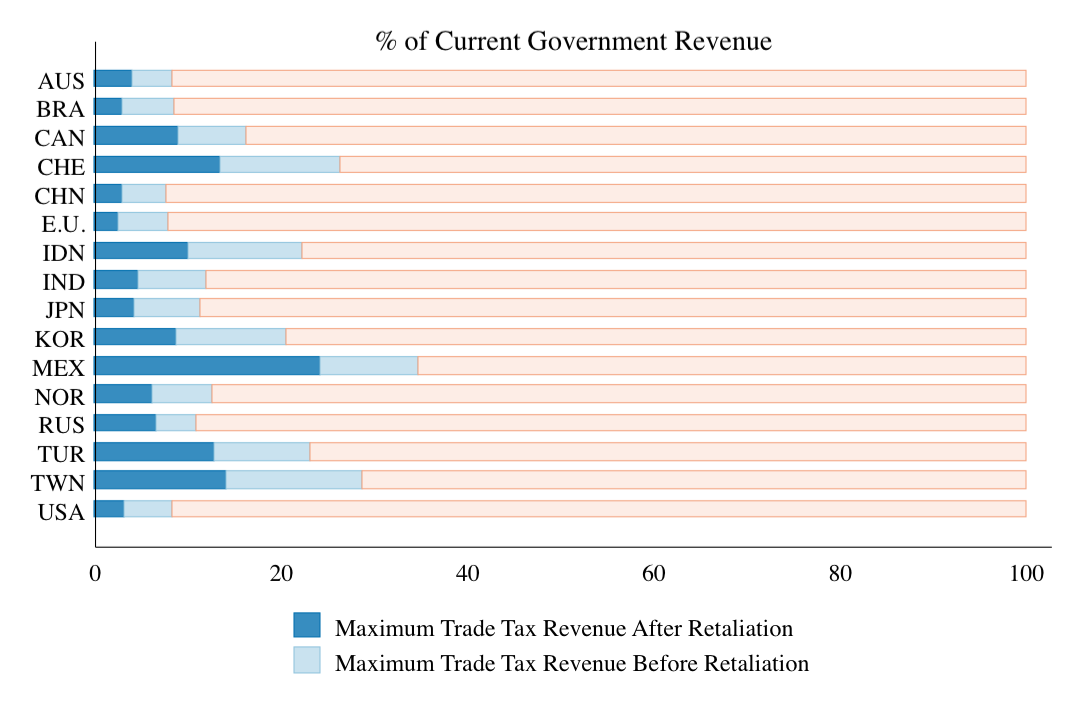
\includegraphics[scale=0.75]{Fig_1}
\par\end{centering}
\end{figure}
\begin{result} 

After retaliation, the trade tax revenues collected by non-cooperative
countries decline by 50\%. Also, every \$1 million of income tax revenue
that was replaced with trade tax revenue imposes an excess burden
of \$2.7 million on the economy. 

\end{result}

Figure \ref{fig:The (Un)Effectiveness} illustrates the first part
of the above result. To document the second part, I follow \citet{kay1980deadweight}
and calculate the \emph{excess burden} of trade taxes as follows:
\[
\textrm{EB}_{i}=e(\{P'_{i},w'_{i}\},W'_{i})-e(\{P{}_{i},w_{i}\},W{}_{i}')-\Delta\mathcal{R}{}_{i}-(\delta_{i}'w'_{i}L'_{i}-\delta_{i}w{}_{i}L),
\]
where $e(.)$ is the expenditure function and $\Delta\mathcal{R}_{i}$
denotes the increase in trade tax revenue. As shown in Appendix \ref{sec: Excess Burden},
the above equation can be reformulated as
\begin{equation}
\textrm{EB}_{i}=Y_{i}\hat{Y}_{i}\left(1-1/\hat{P}_{i}\right)-w_{i}L_{i}\left(\widehat{w_{i}L_{i}}-\hat{L}_{i}\right)-\Delta\mathcal{R}{}_{i}-\delta_{i}w_{i}L_{i}\left(\hat{L}_{i}-1\right),\label{eq: EB}
\end{equation}
where $\hat{Y_{i}}$, $\widehat{w_{i}L_{i}}$, $\hat{L}_{i}$, and
$\hat{P}_{i}$ denote the change in total spending, wage income, labor
supply, and consumer price index when governments replace income tax
with trade tax revenue. Using the above equation, I can calculate
the ratio $\textrm{EB}_{i}/\Delta\mathcal{R}_{i}$, which is reported
in the last column of Table \ref{tab:Revenue-Maximizing-trade-taxes}.
It turns out that $\textrm{EB}_{i}/\mathcal{R}_{i}\approx2.5$ for
the average country, which is remarkably high.\footnote{The cost of retaliation is driven by two distinct cost channels: First,
trade taxes distort consumer prices not only $(i)$ between domestic
and imported varieties, but also $(ii)$ across industries. Second,
as highlighted by Proposition 5, trade taxes distort the supply of
labor in each economy. The combination of these two effects leads
to the large welfare losses reported in Table \ref{tab:Revenue-Maximizing-trade-taxes}.} 

The fact that $\textrm{EB}_{i}/\mathcal{R}_{i}$ is excessively high
and rather uniform across countries is best understood from the lens
of Remark 2 from \ref{subsec: Replacing-Income-tax}. Specifically,
a country can collect more trade tax revenue, $\mathcal{R}_{i}$,
if it is a net importer in low-$\theta$ industries. The same country,
however, is also more reliant on trade and experiences a greater loss,
$\textrm{EB}_{i}$ from retaliation. These countervailing effects
imply that $\textrm{EB}_{i}/\mathcal{R}_{i}$ should be rather high
for all countries including those with more national-level market
power. In comparison, the nominal welfare loss, $\Delta W_{i}$, varies
considerably across countries depending on the country's size and
import composition.

It is worth reiterating that Result 2 concerns retaliation by \emph{trade
tax revenue-maximizing} governments. Alternatively, governments can
replace income tax revenue with noncooperative \emph{welfare-maximizing}
trade taxes. In that case, the optimal export tax rate will remain
the same. But optimal import taxes will be uniform to minimize distortions
to local consumer prices. Accordingly, welfare-maximizing trade taxes
will raise less revenue while also imposing a smaller (gross) excess
burden on the economy. But, altogether, the excess burden per dollar
of tax revenue, $\textrm{EB}_{i}/\mathcal{R}_{i}$, should not be
that different under this scenario.

The above result is also related to the findings in \citet{amiti2019cep}
and \citet{fajgelbaum2019return} who analyze the revenue-raising
effects and the excess burden of the Trump administration\textquoteright s
tariffs on China. Unlike the present analysis, both of these studies
analyze \emph{already-applied} tariffs that are targeted solely at
Chinese import goods. \citet{amiti2019cep} estimate that the Trump
administration\textquoteright s tariffs raised \$8.2 billion in revenue
but inflicted an excess burden equal to \$15.6 billion on the U.S.
economy. That implies an excess burden of \$1.9 per dollar of tax
revenue, which is close but slightly lower than the numbers reported
in Table \ref{tab:Revenue-Maximizing-trade-taxes}. A simple explanation
for why \citet{amiti2019cep} find a smaller excess burden per dollar
is that the Trump administration\textquoteright s tariffs $(i)$ were
set lower than the revenue-maximizing rate and $(ii)$ faced only
partial retaliation from China.

\begin{result} 

\emph{{[}The effectiveness-efficiency trade-off{]} }In a cross-section
of countries, trade taxes are the least efficient when they are most
effective at raising revenue. 

\end{result}

The above result is portrayed in Figure \ref{fig: Effectiveness vs. Efficiency}.
For smaller economies, such as Taiwan or Mexico, trade taxes can be
more effective at replacing existing income tax revenues. In these
economies, however, revenue-raising trade taxes are also less efficient.
That is, after prompting retaliation, they impose a greater excess
burden on the economy. The intuition behind this result is similar
to that provided in Section \ref{subsec: Replacing-Income-tax}: Trade
taxes are a more effective fiscal instrument for countries that $(i)$
face a lower import-weighted trade elasticity, and $(ii)$ exhibit
a higher trade-to-GDP ratio. Both of these characteristics, however,
indicate that imported goods are less-substitutable with domestic
alternatives in that country. As a result, reducing trade to raise
tax revenue will have a greater negative effect on welfare.

\begin{figure}
\caption{\label{fig: Effectiveness vs. Efficiency}The Effectiveness vs. Efficiency
Trade-off}

\begin{centering}
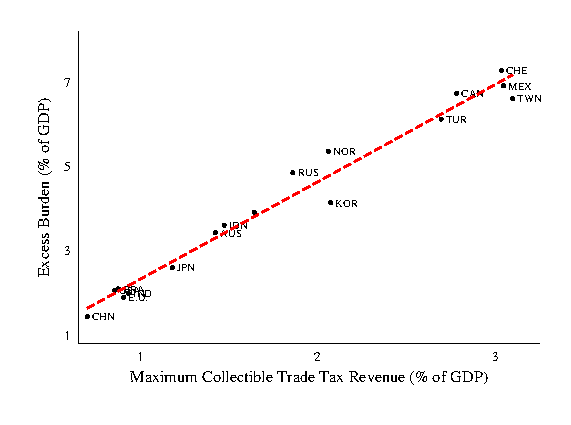
\includegraphics[scale=1.25]{Fig_2}\vspace{-0.15in}
\par\end{centering}
\centering{}%
\noindent\begin{minipage}[t]{1\columnwidth}%
\emph{\footnotesize{}Note}{\footnotesize{}: The x-axis corresponds
to the maximum trade tax revenue (as a share of GDP) that a country
can collect post-retaliation. The y-axis corresponds to the excess
burden of these taxes relative to GDP. }%
\end{minipage}
\end{figure}
\begin{result} 

The gains from trade agreements are 30\% larger once we account for
the fiscal cost of trade wars and distortions to labor supply decisions. 

\end{result}

The gains from trade agreements can be calculated in the same vein
as \citet{ossa2014trade,ossa2016quantitative}. Multilateral trade
agreements avert the cost of full-fledged multilateral trade wars.
So, by construction, the gains from trade agreements equal the welfare
costs of a full-fledged trade war, which are reported in the last
column of Table \ref{tab:Revenue-Maximizing-trade-taxes}. The numbers
produced here, though, account for two cost channels that have been
overlooked in the prior literature. Namely: 
\begin{enumerate}
\item Distortions to labor supply decisions, which are driven by an increase
in consumer price index, $\tilde{P}_{i}$, after the trade war; and
\item A fiscal cost, driven by the shrinking of the income tax base, which
forces governments to raise the income tax rate, $\delta_{i}$, in
order to maintain real government expenditure. 
\end{enumerate}
If we account for these previously-overlooked cost channels, trade
agreements contribute to the average country's real income by 7\%,
which is notably larger than the prior literature estimates. 

To shed further light on these differences, note that the importance
of cost channels $(i)$ and $(ii)$ is regulated by the labor supply
elasticity, $\kappa$. Under the standard assumption that $\kappa=0$,
trade wars do not distort labor supply decisions and neither do they
impose a fiscal cost on the economy.\footnote{When $\kappa=0$, income taxes are non-distortionary. So even if the
trade war shrinks the income tax base it imposes no real fiscal cost
on the economy.} As $\kappa$ increases, however, the importance of cost channels
$(i)$ and $(ii)$ also increases.

Figure \ref{fig: The-fiscal-cost} illustrates this argument and indicates
that the aforementioned effects are profound. The solid line demonstrates
that as $\kappa$ increases from 0 to 0.9, the implied gains from
trade agreements (or the loss from a full-fledged trade war) increases
from less than $5$\% to around $10$\% in terms of real GDP for the
average country. The dashed line demonstrates that, in the event of
a full-fledged trade war, countries have to raise their income tax
rate to counter the shrinking income tax base. The higher the labor
supply elasticity, $\kappa$, the greater the needed increase in $\delta_{i}$,
and the higher the welfare cost of such an increase.\footnote{The statement of \emph{Result 4} derives from comparing the welfare
effects under $\kappa=0$ and $\kappa=0.5$. Doing so implies that
overlooking cost channels $(i)$ and $(ii)$ understates the gains
from trade agreements by more than 30\%.}

\begin{figure}[!tbh]
\caption{\label{fig: The-fiscal-cost}The Fiscal Cost of Trade Wars}
\vspace{-0.05in}
\begin{centering}
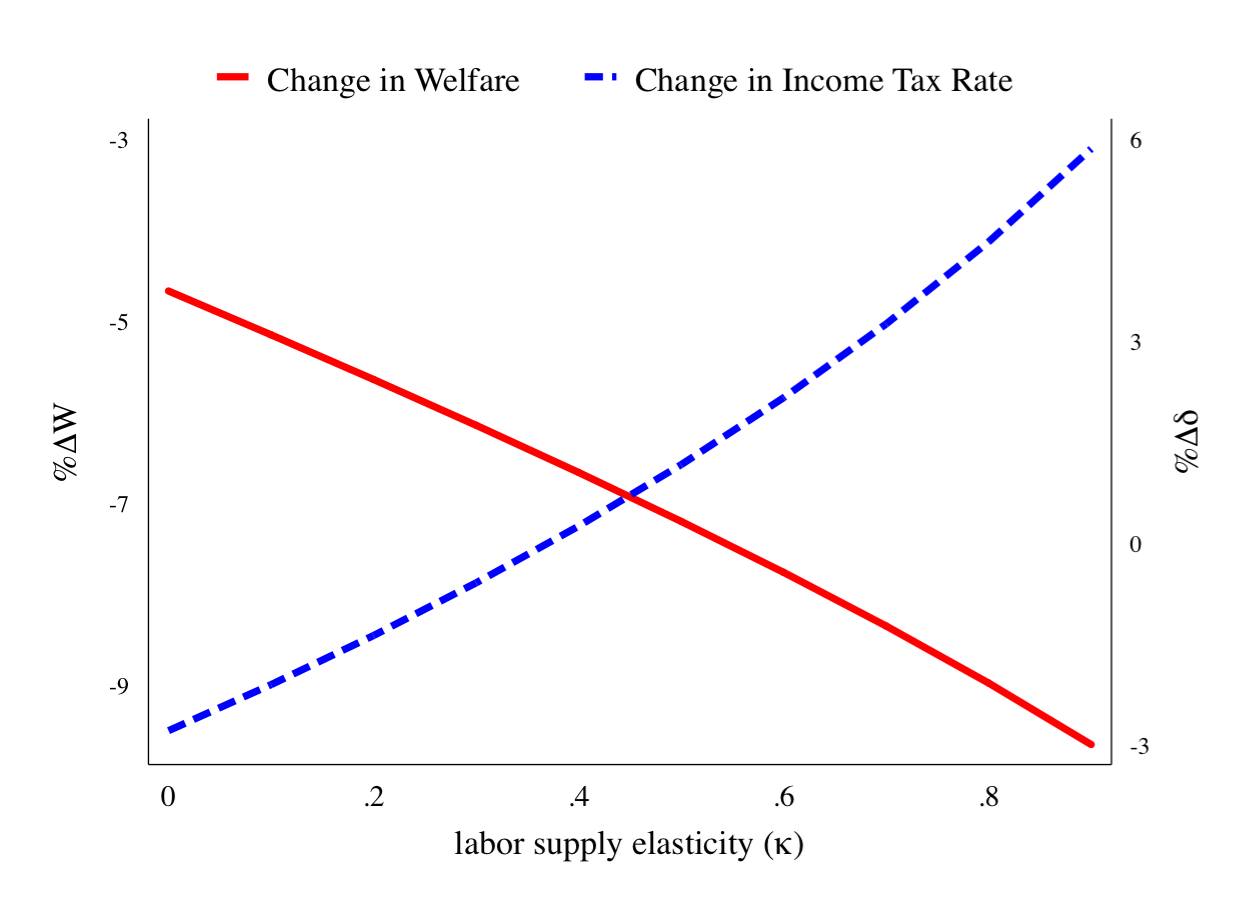
\includegraphics[scale=0.6]{Fig_3}\vspace{-0.15in}
\par\end{centering}
\centering{}%
\noindent\begin{minipage}[t]{1\columnwidth}%
\emph{\footnotesize{}Note}{\footnotesize{}: The solid line reports
the average welfare loss per country after retaliation. The dashed
line reports the change in income tax revenue that is necessary to
maintain real government spending after retaliation. $\kappa$ governs
the importance of distortions to labor supply decisions. When $\kappa=0$,
raising $\delta$ imposes no cost on the economy as labor supply decisions
are unaffected by such a change. The higher the $\kappa$, however,
the higher the cost of raising $\delta$.}%
\end{minipage}
\end{figure}

\section{Conclusion}

The standard argument against \emph{taxing-trade-for-revenue} asserts
that countries are small compared to the rest of the world and bear
the entire cost of their trade taxes. In this line of argument, trade
taxes are strictly less-efficient than other revenue-raising tax instruments,
even without retaliation by trading partners. For all its merits,
this argument does not paint a complete picture for two reasons. First,
if the recent political climate is of any indication, governments
occasionally have a political or institutional preference for trade
taxation. For such governments, whether to erect trade taxes or not
is a matter of effectiveness rather than efficiency. Second, as established
by \citet{alvarez2007general}, even small countries can gain non-cooperatively
from trade taxation if we account for technology differentiation and
general equilibrium policy effects. 

Against this backdrop, I presented an alternative argument against
\emph{taxing-trade-for-revenue}. One that was based on two independent
assertions: First, I argued that trade taxes are an ineffective fiscal
instrument. To this end, I estimated the degree of national-level
market power across various industries and countries. Using these
estimates, I demonstrated that (even before retaliation) the average
country can beneficially replace only 16\% of its domestic tax revenues
with trade taxes. Second, I demonstrated that half of these revenues
disappear after retaliation. Moreover, governments are forced to increase
domestic taxes after retaliation to counter the shrinking domestic
tax base.

The above results were produced with a new \emph{sufficient statistics}
methodology that improves upon standard techniques commonly employed
in the quantitative trade policy literature. As noted in Section \ref{sec:Theoretical-Model},
this new methodology readily extends to environments featuring $(i)$
worker heterogeneity, $(ii)$ pre-existing market distortions, and
$(ii)$ a variable unit labor cost. Mapping these extensions to actual
data provides a fruitful avenue for future research. The cost of performing
such extended analyses is that they require additional data collection
on within-country patterns of employment, markup wedges, and cost
functions. The benefit of conducting such analyses is determining
whether \emph{taxing-trade-for-revenue} exacerbates pre-existing market
distortions or worsens income inequality.

\bibliographystyle{chicago}
\bibliography{Trade_Tax_Revenue}

\clearpage{}

\pagenumbering{arabic}
\renewcommand*{\thepage}{A\arabic{page}}

\appendix


\section{\label{sec:Proof-of-Lemma}Proof of Lemma 1}

\paragraph*{Reformulating the Model in Terms of Aggregate Quantities and Prices:}

The proof can be simplified if we convert the EK model to an observationally
equivalent Armington model, and appeal to existing results in consumer
theory. The Armington-equivalent of the EK model features a utility
function, $U_{i}=\prod_{k=1}^{K}\left(\sum_{j}Q_{ji,k}^{\rho_{k}}\right)^{e_{i,k}/\rho_{k}}$,
that aggregates over various composite national-level varieties, with
$\rho_{k}=\theta_{k}/1+\theta_{k}$. The aggregate CES demand facing
composite variety $ji,k$ (export $j$--importer $i$, industry $k$)
can be expressed as
\[
Q_{ji,k}\equiv\mathcal{D}_{ji,k}\left(\boldsymbol{\tilde{P}}_{i},Y_{i}\right)=\tilde{P}_{ji,k}^{-1-\theta_{k}}\ \tilde{P}_{i,k}^{\theta_{k}}\ Y_{i}
\]
where $\tilde{P}_{ji,k}$ is the consumer price index of composite
$ji,k$; with $\tilde{P}_{i,k}=\left(\sum_{j=1}^{N}\tilde{P}_{ji,k}^{-\theta_{k}}\right)^{-1/\theta_{k}}$.
The consumer price is $\tilde{P}_{ji,k}=(1+x_{ji,k})(1+t_{ji,k})P_{ji,k}$,
with the producer price given by $P_{ji,k}=\tau_{ji,k}T_{j}^{-\frac{1}{\theta_{k}}}w_{j}$.\footnote{One can think of $\tau_{ji,k}T_{j}^{-\frac{1}{\theta_{k}}}$ as the
unit labor cost production and transportation.} Under this formulation, equilibrium is characterized by Equations
\ref{eq: Eq Income} and \ref{eq: Eq Wage}, noting that $\lambda_{ji,k}=\left(\tilde{P}_{ji,k}/\tilde{P}_{i,k}\right)^{-\theta_{k}}.$

\paragraph*{Additional Notation.}

The goal is toe prove that for any $a\in\mathbb{R}_{+}$, the feasible
wage-tax combination $A\equiv(\boldsymbol{1}+\boldsymbol{t}{}_{i},\boldsymbol{t}{}_{-i},\boldsymbol{1}+\boldsymbol{x}{}_{i},\boldsymbol{x}{}_{-i},\boldsymbol{\delta};w{}_{i},\boldsymbol{w}{}_{-i})$
is equivalent to the following wage-tax combination from a welfare
standpoint:
\[
A'\equiv(\boldsymbol{1}+\boldsymbol{t}'_{i},\boldsymbol{t}'_{-i},\boldsymbol{1}+\boldsymbol{x}'_{i},\boldsymbol{x}'_{-i},\boldsymbol{\delta}';w'_{i},\boldsymbol{w}'_{-i})=(a(\boldsymbol{1}+\boldsymbol{t}_{i}),\boldsymbol{t}_{-i},(\boldsymbol{1}+\boldsymbol{x}_{i})/a,\boldsymbol{x}_{-i},\boldsymbol{\delta};aw_{i},\boldsymbol{w}_{-i})
\]
To present the proof, I will adopt the following notation: For a generic
variable that assumes value $Z$ under combination $A$, $Z'$ denotes
the equilibrium value of the same variable under combination $A'$.
Namely,
\[
Z\equiv\mathcal{Z}(\boldsymbol{x},\boldsymbol{t},\boldsymbol{\delta},\boldsymbol{w});\ \ \ \ \ \ \ \ \ \ Z'\equiv\mathcal{Z}(\boldsymbol{x}',\boldsymbol{t}',\boldsymbol{\delta}',\boldsymbol{w}')
\]
For instance $Y'_{i}$ denotes the national income in country $i$
under the wage-tax combination $A'$. The same goes for any other
variable like $\tilde{P}'_{ji,k}$ or $Q'_{ji,k}$. 

\paragraph*{Proof based on Two Intermediate Claims.}

Invoking the above choice of notation, the proof of Lemma 1 follows
from two intermediate claims, labeled $\textrm{C1}$and $\textrm{C2}$.
Claim C1 can be states as follows, and derives from the Marshallian
demand function $\mathcal{Q}_{ji,k}\left(\boldsymbol{\tilde{P}}_{i},Y_{i}\right)$
being homogeneous of degree zero: 
\[
\begin{cases}
\boldsymbol{\tilde{P}}'_{i}=a\boldsymbol{\tilde{P}}_{i};\ \ Y'_{i}=aY_{i}\\
\boldsymbol{\tilde{P}}'_{j}=\boldsymbol{\tilde{P}}_{j};\ \ Y'_{j}=Y_{j} & j\neq i
\end{cases}\ \Longrightarrow\ \begin{cases}
Q'_{ij,k}=Q_{ij,k} & \forall k\\
Q'_{ji,k}=Q_{ji,k} & \forall k
\end{cases}.\ \ \ (\textrm{C1})
\]
Recall that $\tilde{\boldsymbol{P}_{i}}\equiv\{\tilde{P}_{ji,k}\}_{j,k}$
denotes the entire vector of consumer prices in market $i$. Claim
C2 can be stated as follows 
\[
\begin{cases}
Q'_{ij,k}=Q_{ij,k} & \forall k\\
Q'_{ji,k}=Q_{ji,k} & \forall k
\end{cases}\ \Longrightarrow\ \begin{cases}
\boldsymbol{\tilde{P}}'_{i}=a\boldsymbol{\tilde{P}}_{i};\ \ Y'_{i}=aY_{i}\\
\boldsymbol{\tilde{P}}'_{j}=\boldsymbol{\tilde{P}}_{j};\ \ Y'_{j}=Y_{j} & j\neq i
\end{cases}.\ \ \ (\textrm{C2})
\]
The fact that $\boldsymbol{\tilde{P}}'_{i}=a\boldsymbol{\tilde{P}}_{i}$
and $\boldsymbol{\tilde{P}}'_{j}=\boldsymbol{\tilde{P}}_{j}$ follow
trivially from the equilibrium expression for prices. Specifically,
defining $\bar{\rho}_{nj,k}\equiv\tau_{nj,k}T_{n}^{-\frac{1}{\theta_{k}}}$,
{\small \[
\hspace{-0.25in} \tilde{P}'_{nj,k}=\bar{\rho}_{nj,k}(1+x'_{nj,k})(1+t'_{nj,k})w'_{n}=\begin{cases}
\bar{\rho}_{ni,k}(1+x_{ni,k})\times a(1+t{}_{ni,k})\times w{}_{n}=a\tilde{P}_{ni,k} & j=i,\ n\neq i\\
\bar{\rho}_{ii,k}\times aw{}_{i}=a\tilde{P}_{ii,k} & j=i,\ n=i\\
\bar{\rho}_{nj,k}(1+x{}_{nj,k})(1+t{}_{nj,k})w{}_{n}=\tilde{P}_{nj,k} & j\neq i,\ n\neq i\\
\bar{\rho}_{ij,k}\frac{(1+x_{ij,k})}{a}(1+t{}_{ij,k})\times aw{}_{i}=\tilde{P}_{ij,k} & j=i,\ n\neq i
\end{cases}.
\]}
That $Y'_{j}=Y_{j}$ for all $j\neq i,$ follows immediately from
$Q'_{ji,k}=Q_{ji,k}$ and $\boldsymbol{\tilde{P}}'_{j}=\boldsymbol{\tilde{P}}_{j}$.
The fact that $Y'_{i}=aY_{i}$ can be established along the following
steps:
{\small\begin{align*}
Y'_{i} & =w'_{i}L'_{i}+\sum_{j,k}\left[\frac{t'_{ji,k}}{1+t'_{ji,k}}\tilde{P}'_{ji,k}Q'_{ji,k}+\frac{x'_{ij,k}}{(1+t_{ij,k})(1+x'_{ij,k})}\tilde{P}'_{ij,k}Q'_{ij,k}\right]\\
 & =aw_{i}L{}_{i}+\sum_{j,k}\left[\left(a-\frac{a}{a(1+t_{ji,k})}\right)\tilde{P}{}_{ji,k}Q{}_{ji,k}+\left[\frac{1}{1+t_{ij,k}}-\frac{1}{(1+t_{ij,k})(1+x{}_{ij,k})/a}\right]\tilde{P}{}_{ij,k}Q{}_{ij,k}\right]\\
 & =aw_{i}L{}_{i}+\sum_{j,k}\left[a\tilde{P}{}_{ji,k}Q{}_{ji,k}+\frac{a}{(1+t_{ij,k})(1+x{}_{ij,k})}\tilde{P}{}_{ij,k}Q{}_{ij,k}\right]\\
 & =aw_{i}L{}_{i}+a\sum_{j,k}\left[\frac{t_{ji,k}}{1+t_{ji,k}}\tilde{P}{}_{ji,k}Q{}_{ji,k}+\frac{1}{(1+t_{ij,k})(1+x{}_{ij,k})}\tilde{P}{}_{ij,k}Q{}_{ij,k}\right]=a\left(w_{i}L_{i}+\mathcal{R}_{i}\right),
\end{align*}}
where the second and last line follow from the balanced trade condition,
i.e., $\sum_{j,k}\left[\frac{\tilde{P}{}_{ji,k}Q{}_{ji,k}}{1+t_{ji,k}}-\frac{\tilde{P}{}_{ij,k}Q{}_{ij,k}}{1+t_{ij,k}}\right]=0.$
Together, Claims $\textrm{C1}$ and $\textrm{C2}$ indicate that the
vector of consumption quantities are identical under combinations
$A$ and $A'$. That is for any $a\in\mathbb{R}_{+}$, $Q'_{ji,k}=Q_{ji,k}$
for all $ji,k$. As such welfare is preserved if we switch from the
wage-tax combination $A$ to $A'$, thereby establishing Lemma 1. 

\section{\label{sec: Proof-of-Proposition 1}Proof of Theorem 1}

\paragraph*{Step 1.}

As with Lemma 1, the proof can be simplified if we convert the EK
model to an observationally equivalent Armington model. To repeat
myself, the Armington-equivalent of the EK model features a utility
function, $U_{i}=\prod_{k=1}^{K}\left(\sum_{j}Q_{ji,k}^{\rho_{k}}\right)^{e_{i,k}/\rho_{k}}$,
that aggregates over various composite national-level varieties, with
$\rho_{k}=\theta_{k}/1+\theta_{k}$. The aggregate CES demand facing
composite variety $ji,k$ (export $j$--importer $i$, industry $k$)
can be expressed as
\[
Q_{ji,k}\equiv\mathcal{Q}_{ji,k}\left(\boldsymbol{\tilde{P}}_{i},Y_{i}\right)=\tilde{P}_{ji,k}^{-1-\theta_{k}}\ \tilde{P}_{i,k}^{\theta_{k}}\ Y_{i}
\]
where $\tilde{P}_{ji,k}$ is the consumer price index of composite
$ji,k$; with $\tilde{P}_{i,k}=\left(\sum_{j=1}^{N}\tilde{P}_{ji,k}^{-\theta_{k}}\right)^{-1/\theta_{k}}$.
Based on the above demand function, we can define
\begin{enumerate}
\item {[}Price elasticity demand{]} $\varepsilon_{ji,k}^{(\jmath i,g)}\equiv\partial\ln\mathcal{Q}_{ji,k}(.)/\partial\ln\tilde{P}_{\jmath i,k}$;
\item {[}Income elasticity of demand{]} $\eta_{ji,k}=\partial\ln\mathcal{Q}_{ji,k}(.)/\partial\ln Y_{i}$.
\end{enumerate}
Furthermore, the indirect utility of the representative consumer is
given by $V_{i}(\boldsymbol{\tilde{P}}_{i},Y_{i})=Y_{i}/\prod_{k=1}^{K}\tilde{P}_{i,k}^{e_{i,k}}$.
The consumer price is $\tilde{P}_{ji,k}=(1+x_{ji,k})(1+t_{ji,k})P_{ji,k}$,
with the producer price given by $P_{ji,k}=\tau_{ji,k}T_{j}^{-\frac{1}{\theta_{k}}}w_{j}$.\footnote{One can think of $\tau_{ji,k}T_{j}^{-\frac{1}{\theta_{k}}}$ as the
unit labor cost production and transportation.} Finally, equilibrium is characterized by Equations \ref{eq: Eq Income}
and \ref{eq: Eq Wage}, noting that $\lambda_{ji,k}=\left(\tilde{P}_{ji,k}/\tilde{P}_{i,k}\right)^{-\theta_{k}}.$

\paragraph*{Step 2.}

This step simplifies the notation by shrinking the variable space,
as well as converting Problem P1 into an inner (unrestricted) problem
and an outer problem. We can simplify the notation by combining and
simultaneously solving Equation \ref{eq: Eq Income} for various countries:
\begin{equation}
\begin{cases}
Y_{1}=w_{1}L_{1}(\boldsymbol{t},\boldsymbol{x},\boldsymbol{\delta};\boldsymbol{w})+\mathcal{R}_{1}(\boldsymbol{t},\boldsymbol{x},\boldsymbol{\delta};\boldsymbol{w},\boldsymbol{Y})\\
\vdots\\
Y_{N}=w_{N}L_{N}(\boldsymbol{t},\boldsymbol{x},\boldsymbol{\delta};\boldsymbol{w})+\mathcal{R}_{N}(\boldsymbol{t},\boldsymbol{x},\boldsymbol{\delta};\boldsymbol{w},\boldsymbol{Y})
\end{cases}.\label{eq: sys Y}
\end{equation}
The above system of equations uniquely solves $\boldsymbol{Y}$ in
terms of $(\boldsymbol{t},\boldsymbol{x},\boldsymbol{\delta};\boldsymbol{w})$.
Using the corresponding solution, each endogenous variable $x(\boldsymbol{t},\boldsymbol{x},\boldsymbol{\delta};\boldsymbol{w})$
can be re-formulated as a function applied taxes across the world
as well the equilibrium wage vector, $\boldsymbol{w}$, that is consistent
with these taxes. Correspondingly, Country $i$'s trade tax revenue
can be expressed as follows:
\begin{align}
\mathcal{R}_{i}(\boldsymbol{t}_{i},\boldsymbol{x}_{i},\boldsymbol{t}_{-i},\boldsymbol{x}_{-i},\boldsymbol{\delta};\boldsymbol{w},\boldsymbol{Y})\equiv & \mathcal{R}_{i}(\boldsymbol{t}_{i},\boldsymbol{x}_{i},\boldsymbol{t}_{-i},\boldsymbol{x}_{-i},\boldsymbol{\delta};\boldsymbol{w},\boldsymbol{Y}(\boldsymbol{t},\boldsymbol{x},\boldsymbol{\delta};\boldsymbol{w}))\label{eq: Revneue Function}
\end{align}
Problem P1 can be, therefore, formulated as
\begin{align*}
\max_{\boldsymbol{t}_{i},\boldsymbol{x}_{i}}\ \  & \mathcal{R}_{i}(\boldsymbol{t}_{i},\boldsymbol{x}_{i},\boldsymbol{t}_{-i},\boldsymbol{x}_{-i},\boldsymbol{\delta};\boldsymbol{w},\boldsymbol{Y})\\
s.t. & \ \ \delta w_{i}L_{i}+\mathcal{R}_{i}(.)=\overline{G}_{i}.
\end{align*}
We can further simplify the above problem by appealing to Lemma 1.
Specifically, based on Lemma 1, multiple trade tax schedules that
maximize the share of trade tax revenue in total government revenue.
Hence, we can solve Problem P1 without enforcing the revenue-preserving
constraint (inner problem). After we obtain a solution to the unrestricted
problem, we can identify the solution of interest by an across-the-board
shift in export and import taxes (outer problem). Assuming that the
problem is well-behaved, i.e., $\varepsilon_{ji,k}^{(ji,k)}<-1$,
the first-order conditions (FOCs) characterizing the inner problem
can be stated as:\footnote{In the above system of equation, with a slight abuse of notation,
$\left(\frac{\partial\mathcal{R}_{i}(.)}{\partial\ln(1+t_{ji,k})}\right)_{\boldsymbol{w}}\equiv\left(\frac{\partial\mathcal{R}_{i}(.)}{\partial\ln(1+t_{ji,k})}+\frac{\partial\mathcal{R}_{i}(.)}{\partial\ln\boldsymbol{Y}}\frac{\partial\boldsymbol{Y}}{\partial\ln(1+t_{ji,k})}\right)_{\boldsymbol{w}}$
and $\frac{\partial\mathcal{R}_{i}(.)}{\partial\ln\boldsymbol{w}}\equiv\frac{\partial\mathcal{R}_{i}(.)}{\partial\ln\boldsymbol{w}}+\frac{\partial\mathcal{R}_{i}(.)}{\partial\ln\boldsymbol{Y}}\frac{\partial\boldsymbol{Y}}{\partial\ln\boldsymbol{w}}$,
where the partial derivatives $\frac{\partial\boldsymbol{Y}}{\partial\ln(1+t_{ji,k})}$
and $\frac{\partial\boldsymbol{Y}}{\partial\ln\boldsymbol{w}}$ are
implied by the System of Equations \ref{eq: sys Y}.}
\begin{equation}
\begin{cases}
\frac{\text{d}\mathcal{R}_{i}(.)}{\text{d}\ln(1+t_{ji,k})}=\left(\frac{\partial\mathcal{R}_{i}(.)}{\partial\ln(1+t_{ji,k})}\right)_{\boldsymbol{w}}+\sum_{\jmath=1}^{N}\left[\left(\frac{\partial\mathcal{R}_{i}(.)}{\partial\ln w_{\jmath}}\right)_{\boldsymbol{w}_{-\jmath}}\frac{\text{d}\ln w_{\jmath}}{\text{d}\ln(1+t_{ji,k})}\right] & \forall j,k\\
\frac{\text{d}\mathcal{R}_{i}(.)}{\text{d}\ln(1+x_{ij,k})}=\left(\frac{\partial\mathcal{R}_{i}(.)}{\partial\ln(1+x_{ij,k})}\right)_{\boldsymbol{w}}+\sum_{\jmath=1}^{N}\left[\left(\frac{\partial\mathcal{R}_{i}(.)}{\partial\ln w_{\jmath}}\right)_{\boldsymbol{w}_{-\jmath}}\frac{\text{d}\ln w_{\jmath}}{\text{d}\ln(1+x_{ij,k})}\right] & \forall j,k
\end{cases},\label{eq: FOC}
\end{equation}
where $\left(\frac{\partial\mathcal{R}_{i}(.)}{\partial\ln(1+t_{ji,k})}\right)_{\boldsymbol{w}}$
denotes the partial derivative w.r.t. $1+t_{ji,k}$, holding the entire
vector of wages $\boldsymbol{w}$ constant.

\paragraph*{Step 3.}

The System of FOCs (\ref{eq: FOC}) can be simplified, to a first-order
approximation, along the following steps. First, note that
{\small
\begin{align}
\hspace{-0.7in}\left(\frac{\partial\mathcal{R}_{i}(.)}{\partial\ln w_{\jmath}}\right)_{\boldsymbol{w}_{-\jmath}} & =\sum_{k}\sum_{\ell}\left[t_{\ell i,k}P_{\ell i,k}Q_{\ell i,k}\left(\frac{\partial\ln P_{\ell i,k}Q_{\ell i,k}}{\partial\ln w_{\jmath}}\right)_{\boldsymbol{w}_{-\jmath}}\right]=\sum_{k}\sum_{\ell}\left[t_{\ell i,k}P_{\ell i,k}Q_{\ell i,k}\left(\mathbbm{1}\left\{ \ell=\jmath\right\} +\varepsilon_{\ell i,k}^{(\jmath i,k)}\right)\right]\nonumber \\
\hspace{-0.7in} & =\sum_{k}\sum_{\ell}\theta_{k}t_{\ell i,k}P_{\ell i,k}Q_{\ell i,k}\lambda_{\jmath i,k}-\sum_{k}t_{\jmath i,k}P_{\ell i,k}Q_{\ell i,k}=Y_{i}\sum_{k}\left[\theta_{k}\left(\overline{\frac{t_{i,k}}{1+t_{i,k}}}-\frac{t_{\jmath i,k}}{1+t_{\jmath i,k}}\right)\frac{\lambda_{\jmath i,k}}{\lambda_{\jmath i}}\right]\lambda_{\jmath i},\label{eq: dR/dw}
\end{align}} where $\lambda_{\jmath i}=\sum_{k}\lambda_{\jmath i,k}e_{i,k}$.
Second, to determine $\text{d}\ln\boldsymbol{w}/\text{d}\ln(1+\boldsymbol{t}_{i})$,
we can apply the Implicit Function Theorem to the system of labor
market clearing conditions:
\[
\begin{cases}
S_{1}(\boldsymbol{t},\boldsymbol{x},\boldsymbol{\delta};\boldsymbol{w})\equiv w_{1}L_{1}(\boldsymbol{t},\boldsymbol{x},\boldsymbol{\delta};\boldsymbol{w})-\sum_{i}P_{1i}(\boldsymbol{t},\boldsymbol{x},\boldsymbol{\delta};\boldsymbol{w})Q_{1i}(\boldsymbol{t},\boldsymbol{x},\boldsymbol{\delta};\boldsymbol{w})=0\\
\vdots\\
S_{N}(\boldsymbol{t},\boldsymbol{x},\boldsymbol{\delta};\boldsymbol{w})\equiv w_{N}L_{N}(\boldsymbol{t},\boldsymbol{x},\boldsymbol{\delta};\boldsymbol{w})-\sum_{i}P_{Ni}(\boldsymbol{t},\boldsymbol{x},\boldsymbol{\delta};\boldsymbol{w})Q_{Ni}(\boldsymbol{t},\boldsymbol{x},\boldsymbol{\delta};\boldsymbol{w})=0
\end{cases}.
\]
This application yields the following expression:
\[
\frac{\text{d}\ln\boldsymbol{w}}{\text{d}\ln(\boldsymbol{1}+\boldsymbol{t}_{i})}=-\frac{\partial\boldsymbol{S}(.)}{\partial\ln\boldsymbol{w}}^{-1}\left(\frac{\partial\boldsymbol{S}(.)}{\partial\ln(\boldsymbol{1}+\boldsymbol{t}_{i})}\right)_{\boldsymbol{w}}.
\]
Noting from actual trade data that $r_{\jmath i,k}\lambda_{\ell i,k}\lambda_{ji,k}\approx0$
if $j,\ell\neq i$, the above equation implies that
\begin{equation}
\frac{\text{d}\ln w_{\jmath}}{\text{d}\ln(1+t_{ji,k})}\approx\begin{cases}
\frac{\theta_{k}r_{\jmath i,k}\lambda_{ji,k}}{1+\sum_{\iota}\sum_{g}\theta_{g}r_{\jmath\iota,g}} & \textrm{if }\jmath\neq j,i\\
\frac{\kappa\lambda_{ji,k}+\theta_{k}r_{\jmath i,k}\lambda_{ji,k}}{1+\kappa+\sum_{\iota}\sum_{g}\theta_{g}r_{\jmath\iota,g}} & \textrm{if }\jmath=i
\end{cases}.\label{eq: dw/d1+t}
\end{equation}

Combining Equations \ref{eq: dR/dw} and \ref{eq: dw/d1+t}, indicates
that $\frac{\partial\mathcal{R}_{i}}{\partial\ln w_{\jmath}}\frac{\text{d}\ln w_{\jmath}}{\text{d}\ln(1+t_{ji,k})}\propto r_{\jmath i,k}\lambda_{\jmath i}\lambda_{ji,k}$
if $\jmath\neq j,i$. Hence, given that $r_{\jmath i,k}\lambda_{\jmath i}/r_{ii,k}\lambda_{ii,k}\approx0$,
the system of first-order conditions can be approximated as
\[
\begin{cases}
\frac{\text{d}\mathcal{R}_{i}(.)}{\text{d}\ln(1+t_{ji,k})}\approx\left(\frac{\partial\mathcal{R}_{i}(.)}{\partial\ln(1+t_{ji,k})}\right)_{\boldsymbol{w}}+\left(\frac{\partial\mathcal{R}_{i}(.)}{\partial\ln w_{i}}\right)_{\boldsymbol{w}_{-i}}\frac{\text{d}\ln w_{i}}{\text{d}\ln(1+t_{ji,k})} & \forall j,k\\
\frac{\text{d}\mathcal{R}_{i}(.)}{\text{d}\ln(1+x_{ij,k})}\approx\left(\frac{\partial\mathcal{R}_{i}(.)}{\partial\ln(1+x_{ij,k})}\right)_{\boldsymbol{w}}+\left(\frac{\partial\mathcal{R}_{i}(.)}{\partial\ln w_{i}}\right)_{\boldsymbol{w}_{-i}}\frac{\text{d}\ln w_{i}}{\text{d}\ln(1+x_{ij,k})} & \forall j,k
\end{cases}.
\]


\paragraph*{Step 4.}

As noted earlier, the F.O.C. w.r.t. to import tax, $t_{ji,k}$, can
be formulated as follows:
\[
\left(\frac{\partial\mathcal{R}_{i}(.)}{\partial\ln(1+t_{ji,k})}\right)_{\boldsymbol{w}}+\left(\frac{\partial\mathcal{R}_{i}(.)}{\partial\ln w_{i}}\right)_{\boldsymbol{w}_{-i}}\frac{\text{d}\ln w_{i}}{\text{d}\ln(1+t_{ji,k})}=0
\]
where the first term denotes the effect of $t_{ji,k}$, holding $w_{i}$
and country $i$'s other tax variables constant. This term can be
characterized by applying the chain rule to the governments revenue
function as follows:
{\small \begin{align*}
\hspace{-0.25in} \left(\frac{\partial\mathcal{R}_{i}(.)}{\partial\ln(1+t_{ji,k})}\right)_{\boldsymbol{w}}=\tilde{P}_{ji,k}Q_{ji,k} & +\sum_{g}\sum_{\jmath\neq i}\left(t_{\jmath i,g}(1+x_{\jmath i,g})P_{\jmath i,g}Q_{\jmath i,g}\frac{\partial\ln\mathcal{Q}_{\jmath i,g}(.)}{\partial\ln\tilde{P}_{ji,k}}\frac{\partial\ln\tilde{P}_{ji,k}}{\partial\ln(1+t_{ji,k})}\right) \\
 & +\sum_{g}\sum_{\jmath}\left(t_{\jmath i,g}(1+x_{\jmath i,g})P_{\jmath i,g}Q_{\jmath i,g}\frac{\partial\ln\mathcal{Q}_{\jmath i,g}(.)}{\partial\ln Y_{i}}\right)\left(\frac{\partial\ln Y_{i}}{\partial\ln(1+t_{ji,k})}\right)_{\boldsymbol{w}}.
\end{align*}}
The first term on the right-hand side account for direct arithmetic
effect of $t_{ji,k}$ on tax revenues. The second term accounts for
cross-demand effects. The last term account for general equilibrium
income effects. Note that $\left(\partial\ln Y_{i}/\partial\ln(1+t_{ji,k})\right)_{\boldsymbol{w}}$
encapsulates the partial effect of $t_{ji,k}$ on national income
through both the labor supply and the tax revenue channels. Invoking
our earlier notation for reduced-form Marshallian demand elasticities,
we can simplify the above expression as follows:
\begin{align}
\left(\frac{\partial\mathcal{R}_{i}(.)}{\partial\ln(1+t_{ji,k})}\right)_{\boldsymbol{w}}= & \tilde{P}_{ji,k}Q_{ji,k}+\sum_{g}\sum_{\jmath\neq i}\left(t_{\jmath i,g}(1+x_{\jmath i,g})P_{\jmath i,g}Q_{\jmath i,g}\varepsilon_{\jmath i,g}^{(ji,k)}\right)\nonumber \\
 & +\sum_{g}\sum_{\jmath}\left[t_{\jmath i,g}(1+x_{\jmath i,g})P_{\jmath i,g}Q_{\jmath i,g}\eta_{\jmath i,g}\right]\left(\frac{\partial\ln Y_{i}}{\partial\ln(1+t_{ji,k})}\right)_{\boldsymbol{w}}\label{eq: FOC t}
\end{align}
To characterize the general equilibrium wage effects, we need to determine
$\frac{\text{d}\ln w_{i}}{\text{d}\ln(1+t_{ji,k})}$. This can be
done by applying the Implicit Function Theorem to the country $i$'s
balanced trade condition, $\textrm{BT}_{i}(\boldsymbol{t},\boldsymbol{x},\boldsymbol{\delta};\boldsymbol{w})=\sum_{g}\sum_{j\neq i}\left[(1+x_{ji,g})P_{ji,g}Q_{ji,g}-(1+x_{ij,g})P_{ij,g}Q_{ij,g}\right]$:\footnote{Note that the balanced trade condition derives from the combination
of the labor market clearing (LMC, Equation \ref{eq: Eq Wage}) condition
and the national-level budget constraint (BC, Equation \ref{eq: Eq Income}).}
\begin{align*}
\frac{\text{d}\ln w_{i}}{\text{d}\ln(1+t_{ji,k})} & =\frac{\left(\partial\textrm{BT}_{i}(.)/\partial\ln(1+t_{ji,k})\right)_{\boldsymbol{w}}}{\left(\partial\textrm{BT}_{i}(.)/\partial\ln w_{i}\right)_{\boldsymbol{w}_{-i}}}\\
 & =\frac{\sum_{g}\sum_{\jmath\neq i}\left((1+x_{\jmath i,g})P_{\jmath i,g}Q_{ji,g}\left[\varepsilon_{\jmath i,g}^{(ji,k)}+\eta_{\jmath i,g}\left(\frac{\partial\ln Y_{i}}{\partial\ln(1+t_{ji,k})}\right)_{\boldsymbol{w}}\right]\right)}{\left(\frac{\partial}{\partial\ln w_{i}}\sum_{g}\sum_{\jmath\neq i}\left[(1+x_{\jmath i,g})P_{\jmath i,g}Q_{\jmath i,g}-(1+x_{i\jmath,g})P_{i\jmath,g}Q_{i\jmath,g}\right]\right)_{\boldsymbol{w}_{-i}}}
\end{align*}
Plugging the above expressions back into the F.O.C.s and defining
$\bar{\tau}_{i}\equiv\left(\frac{\partial\mathcal{R}_{i}}{\partial\ln w_{i}}\right)_{\boldsymbol{w}_{-i}}\left(\frac{\partial\textrm{BT}_{i}(.)}{\partial\ln w_{i}}\right)_{\boldsymbol{w}_{-i}}^{-1}$,
we can produce the following condition:
\[
\tilde{P}_{ji,k}Q_{ji,k}+\sum_{g}\sum_{\jmath\neq i}\left(\left[t_{\jmath i,g}-\bar{\tau}_{i}\right](1+x_{\jmath i,g})P_{\jmath i,g}Q_{\jmath i,g}\varepsilon_{\jmath i,g}^{(ji,k)}\right)+\Delta_{i}\left(\frac{\partial\ln Y_{i}}{\partial\ln(1+t_{ji,k})}\right)_{\boldsymbol{w}}=0
\]
where $\Delta_{i}$ is uniform (non-industry-specific) term, defined
as follows 
\[
\Delta_{i}\equiv\sum_{g}\sum_{\jmath\neq i}\left(\left[t_{\jmath i,g}-\bar{\tau}_{i}\right](1+x_{\jmath i,g})P_{\jmath i,g}Q_{\jmath i,g}\eta_{\jmath i,g}\right)
\]
Following Lemma 1, there are multiple revenue-maximizing tax schedules.
Moreover, there always exists a revenue-maximizing trade tax combination
for which $\Delta_{i}=0$. I, henceforth, focus on this particular
combination. Once, I characterize this solution to the F.O.C.s, the
remaining solutions can be identified using an across-the-board shift
in export and import taxes. 

To simplify Equation \ref{eq: FOC t} , we can appeal to the well-known
result in consumer theory that $\tilde{P}_{ji,k}Q_{ji,k}=-\sum_{g}\sum_{\jmath}\left(\tilde{P}_{\jmath i,g}Q_{\jmath i,g}\varepsilon_{\jmath i,k}^{(ji,g)}\right)$.
Applying this relationship to Equation \ref{eq: FOC t} implies the
following optimality condition:
\begin{equation}
\left(1+\bar{\tau}_{i}\right)\sum_{g}\sum_{\jmath\neq i}\left[(1+x_{\jmath i,g})P_{\jmath i,g}Q_{\jmath i,g}\varepsilon_{\jmath i,g}^{(ji,k)}\right]+\sum_{g}\left(P_{ii,g}Q_{ii,g}\varepsilon_{ii,g}^{(ji,k)}\right)=0\label{eq: FOC t1}
\end{equation}
Given that $(i)$ $\varepsilon_{ji,k}^{(ji,k)}=-1-\theta_{k}(1-\lambda_{ji,k})$;
$(ii)$ $\varepsilon_{ji,k}^{(\jmath i,k)}=\theta_{k}\lambda_{ji,k}$
and $\varepsilon_{ji,k}^{(\jmath i,g)}=0$ if $g\neq k$; as well
as $(iii)$ $(1+x_{ji,k})P_{ji,k}Q_{ji,k}=\lambda_{ji,k}/(1+t_{ji,k})$,
Equation \ref{eq: FOC t1} can be reformulated as
\[
(1+\bar{\tau}_{i})\theta_{k}\sum_{\jmath\neq i}\left(\frac{\lambda_{\jmath i,k}}{1+t_{\jmath i,k}}\lambda_{ji,k}\right)+\theta_{k}\lambda_{ii,k}\lambda_{ji,k}=(1+\theta_{k})(1+\bar{\tau}_{i})\frac{\lambda_{ji,k}}{1+t_{\jmath i,k}},
\]
which immediately implies the following expression for the revenue-maximizing
import tax:
\begin{equation}
\frac{1+t_{ji,k}^{*}}{1+\bar{\tau}_{i}}=\frac{1+\theta_{k}}{\theta_{k}}\left[\sum_{\jmath\neq i}\left(\frac{1+\bar{\tau}_{i}}{1+t_{\jmath i,k}^{*}}\lambda_{\jmath i,k}\right)+\lambda_{ii,k}\right]^{-1}\label{eq: FOC t 2}
\end{equation}
The above equation immediately implies that $t_{ji,k}^{*}=t_{\jmath i,k}^{*}$
for all $j$ and $\jmath\in\mathbb{C}-\{i\}$. Plugging this uniformity
result back into Equation \ref{eq: FOC t 2}, yields the following
formula for revenue-maximizing import taxes:
\[
1+t_{ji,k}^{*}=\left(1+\bar{\tau}_{i}\right)\left(1+\frac{1}{\theta_{k}\lambda_{ii,k}}\right)
\]


\paragraph*{Step 5.}

The F.O.C. w.r.t. to export tax, $x_{ij,k}$, can be stated as follows:
\[
\left(\frac{\partial\mathcal{R}_{i}(.)}{\partial\ln(1+x_{ij,k})}\right)_{\boldsymbol{w}}+\left(\frac{\partial\mathcal{R}_{i}(.)}{\partial\ln w_{i}}\right)_{\boldsymbol{w}_{-i}}\frac{\text{d}\ln w_{i}}{\text{d}\ln(1+x_{ij,k})}=0
\]
Applying the Implicit Function Theorem to Equation \ref{eq: Revneue Function},
while noting that $\partial Y_{i}(.)/\partial\ln(1+t_{ji,k})=\partial\mathcal{R}_{i}(.)/\partial\ln(1+t_{ji,k})$,
implies the following:
\begin{align}
\left(\frac{\partial\mathcal{R}_{i}(.)}{\partial\ln(1+x_{ij,k})}\right)_{\boldsymbol{w}} & =(1+x_{ij,k})P_{ij,k}Q_{ji,k}+\sum_{g}\left(x_{ij,g}P_{ij,g}Q_{ij,g}\varepsilon_{ij,g}^{ij,k}\right),\label{eq: FOC x}\\
 & +\sum_{g}\sum_{\jmath\neq i}\left(t_{\jmath i,g}(1+x_{\jmath i,g})P_{\jmath i,g}Q_{\jmath i,g}\eta_{\jmath i,g}\right)\frac{\partial R_{i}}{\partial Y_{i}}\frac{\partial Y_{i}}{\partial\ln(1+x_{ij,k})}=0.\nonumber 
\end{align}
As before, we can apply the Implicit Function Theorem to the country
$i$'s balanced trade condition, $\textrm{BT}_{i}(\boldsymbol{t},\boldsymbol{x},\boldsymbol{\delta};\boldsymbol{w})$,
to determine $\frac{\text{d}\ln w_{i}}{\text{d}\ln(1+t_{ji,k})}$:
\begin{align*}
\frac{\text{d}\ln w_{i}}{\text{d}\ln(1+x_{ij,k})} & =-\frac{\left(\partial\textrm{BT}_{i}(.)/\partial\ln(1+x_{ij,k})\right)_{\boldsymbol{w}}}{\left(\partial\textrm{BT}_{i}(.)/\partial\ln w_{i}\right)_{\boldsymbol{w}_{-i}}}\\
= & \frac{(1+x_{ij,k})P_{ji,k}Q_{ji,k}+\sum_{g}(1+x_{ij,g})P_{ji,g}Q_{ji,g}\left[\varepsilon_{ji,g}^{ji,k}+\eta_{ji,g}\left(\frac{\partial Y_{i}}{\partial\ln(1+x_{ij,k})}\right)_{\boldsymbol{w}}\right]}{\left(\frac{\partial}{\partial\ln w_{i}}\sum_{g}\sum_{\jmath\neq i}\left[(1+x_{\jmath i,g})P_{\jmath i,g}Q_{\jmath i,g}-(1+x_{i\jmath,g})P_{i\jmath,g}Q_{i\jmath,g}\right]\right)_{\boldsymbol{w}_{-i}}}
\end{align*}
Plugging the above expression back into Equation \ref{eq: FOC x},
and adopting the same definitions for $\bar{\tau}_{i}$ and $\Delta_{i}$
\begin{align}
(1+x_{ij,k})P_{ji,k}Q_{ji,k}+ & \sum_{g}\left(x_{ij,g}P_{ij,g}Q_{ij,g}\varepsilon_{ij,g}^{(ij,k)}\right)+\Delta_{i}\left(\frac{\partial Y_{i}}{\partial\ln(1+x_{ij,k})}\right)_{\boldsymbol{w}}\nonumber \\
+ & \bar{\tau}_{i}\left[(1+x_{ij,k})P_{ji,k}Q_{ji,k}+\sum_{g}\left((1+x_{ij,g})P_{ij,g}Q_{ij,g}\varepsilon_{ij,g}^{(ij,k)}\right)\right]\label{eq: FOC x1}
\end{align}
 Rearranging the above equation; noting that $(i)$ $\varepsilon_{ji,k}^{ji,k}=-1-\theta(1-\lambda_{ji,k})$
and $(ii)$ $\varepsilon_{ji,k}^{(\jmath i,g)}=0$ if $g\neq k$;
as well as setting $\Delta_{i}=0$ based on the underlying multiplicity,
implies the following revenue-maximizing tax formula:
\[
(1+x_{ij,k}^{*})(1+\bar{\tau}_{i})=1+\frac{1}{\theta_{k}(1-\lambda_{ij,k})}.
\]


\paragraph*{Step 6.}

Following Lemma 1, the uniform term$\bar{\tau}_{i}$ is redundant
for the inner problem as it acts as a uniform export and import tax
shifter. Accordingly, the trade tax schedule that maximizes the trade
tax revenue subject to total nominal revenue is described by the following
formula:
\begin{align*}
1+x_{ij,k}^{*}= & \left(1+\bar{t}_{i}\right)^{-1}\left(1+\frac{1}{\theta_{k}(1-\lambda_{ij,k})}\right)\\
1+t_{ji,k}^{*}= & \left(1+\bar{t}_{i}\right)\left(1+\frac{1}{\theta_{k}\lambda_{ii,k}}\right).
\end{align*}
The country-specific tax shifter $1+\bar{t}\in\mathbb{R}_{+}$ is
regulated by the restriction on the total nominal revenue. Given the
Problem $\textrm{P1}$, $\bar{t}_{i}$ is pinned down by the constraint
that $\delta w_{i}L_{i}+\mathcal{R}_{i}(.)=\overline{G}_{i}$ (i.e.,
the outer problem). \emph{Q.E.D.}

\section{\label{sec: Excess Burden}Calculating the Excess Burden}

Following \citet{kay1980deadweight}, the excess burden of substituting
the income tax revenue with trade tax revenue is given by
\[
\textrm{EB}_{i}=e(\{P'_{i},w'_{i}\},W'_{i})-e(\{P{}_{i},w{}_{i}\},W'{}_{i})-\underbrace{\Delta\mathcal{R}{}_{i}-(\delta_{i}'w'_{i}L'_{i}-\delta_{i}w{}_{i}L{}_{i})}_{\Delta\textrm{Total Revenue}},
\]
where $e(.)$ is the (labor-augmented) expenditure function, with
$W_{i}=U_{i}(Q_{i},L_{i})$. The change in total revenue, meanwhile,
consists of the increase in trade tax revenue, $\Delta\mathcal{R}_{i}$,
net of the decline in income tax revenue. The above formula can be
extended and rearranged as follows:
\begin{align*}
\textrm{EB}_{i} & =P_{i}'Q_{i}'-P_{i}Q'_{i}-\left[\left(1-\delta_{i}'\right)w_{i}'-\left(1-\delta_{i}\right)w_{i}\right]L'_{i}-\Delta\mathcal{R}{}_{i}-(\delta_{i}'w'_{i}L'_{i}-\delta_{i}w{}_{i}L{}_{i}).\\
 & =P_{i}'Q_{i}'-P_{i}Q'_{i}-(w_{i}'-w_{i})L'_{i}-\Delta\mathcal{R}{}_{i}-\delta_{i}w_{i}\left(L'_{i}-L_{i}\right),
\end{align*}
where $\left[\left(1-\delta_{i}'\right)w_{i}'-\left(1-\delta_{i}\right)w_{i}\right]L'_{i}$,
in the first line, accounts for the wage income workers lose if they
supply $L'_{i}$ units of labor but are paid a wage $w_{i}$. Combining
the above equation with the hat-algebra notation, we can produce the
following expression
\begin{align*}
\textrm{EB}_{i} & =Y_{i}\left(\hat{Y}_{i}-\hat{Q}_{i}\right)-w_{i}L_{i}\left(\widehat{w_{i}L_{i}}-\hat{L}_{i}\right)-\Delta\mathcal{R}{}_{i}-\delta_{i}w_{i}L_{i}\left(\hat{L}_{i}-1\right),
\end{align*}
where $Y_{i}$, $w_{i}L_{i}$, $\delta_{i}w_{i}L_{i}$ are observable,
while $\hat{Y}_{i}$, $\hat{Q}_{i}=\hat{Y}_{i}/\hat{\tilde{P}_{i}}$
, $\widehat{w_{i}L_{i}}$, $\hat{L}_{i}$, and $\Delta\mathcal{R}{}_{i}$
are given by Proposition \ref{prop: hat-algebra}.

\section{\label{sec: Real Revenue Neut.}Solving P1 subject to \emph{Real}
Revenue Neutrality }

Suppose we want to determine the maximum share of government expenditure
that can be financed from trade taxes \emph{subject to} maintaining
the government's real expenditure. This problem can be stated as follows:
\begin{align*}
\max_{(\boldsymbol{t},\boldsymbol{x},\boldsymbol{\delta};\boldsymbol{w},\boldsymbol{Y})\in\mathbb{F}}\  & \mathcal{R}_{i}\left(\boldsymbol{t}_{i},\boldsymbol{x}_{i};\boldsymbol{t}_{-i},\boldsymbol{x}_{-i},\boldsymbol{\delta};\boldsymbol{w},\boldsymbol{Y}\right)/\delta w_{i}L_{i}\ \ \ \ (\textrm{P1}')\\
s.t. & \ \ [\delta_{i}w_{i}L_{i}+\mathcal{R}_{i}(.)]/\tilde{P}_{i}=\overline{G}_{i},
\end{align*}
where $\bar{G}_{i}$ now denotes the \emph{real} government expenditure
under the status quo. To solve the above problem, we can take the
same approach as we did in Section \ref{subsec: Replacing-Income-tax}.
Specifically, we can split the problem into $(a)$ an unconstrained
lower-tier problem that solves for $\boldsymbol{x}_{i}$ and $\boldsymbol{t}_{i}$
given the choice of $\delta_{i}$, and $(b)$ an upper-tier problem
that chooses $\delta_{i}$ to satisfy the real revenue-neutrality
constraint.

To this end, we can invoke Lemma 1 and follow the same steps conducted
in Appendix \ref{sec: Proof-of-Proposition 1} to solve the unconstrained
lower-tier problem. Doing so implies that for any given choice of
$\delta_{i}$, the optimal trade tax is given by the formula specified
under Theorem 1. The only qualification, here, is that the tax shifter
$\bar{t}_{i}$ is now redundant as it affects neither the objective
function nor the real revenue-neutrality constraint. The solution
to Problem (P1') can therefore be attained by choosing $\delta_{i}$
in order to satisfy the real revenue-neutrality constraint. The following
proposition outlines this claim.
\begin{prop}
\label{prop: revenue-maximizing P1-1} The tax schedule that solves
Problem (P1') includes the following set of trade taxes
\begin{align*}
1+t_{ji,k}^{*}=1+\frac{1}{\theta_{k}\lambda_{ii,k}}, & \ \ \ \forall j\neq i;\ \forall k\in\mathbb{K}\\
1+x_{ij,k}^{*}=1+\frac{1}{\theta_{k}\left(1-\lambda_{ij,k}\right)}, & \ \ \ \forall j\neq i;\ \forall k\in\mathbb{K},
\end{align*}
as well as an income tax, $\delta_{i}$, that is chosen to satisfy
the real revenue neutrality constraint.
\end{prop}
Based on the same idea, we can also produce analogs for Propositions
1 and 2. Specifically, in both cases, the uniform tax shifter can
be set to zero or any other non-negative number. $\delta_{i}$ has
to be, then, chosen to satisfy the real revenue-neutrality constraint.
Correspondingly, we can map the analytic tax formulas to data to compute
the effectiveness of trade taxes at raising revenue before and after
retaliation. This final step is outlined by the following proposition,
which is analog of Proposition \ref{prop: hat-algebra} except that
it include $\hat{\delta}_{i}$ as a free-moving parameter and imposes
the real rather than nominal revenue-neutrality.
\begin{prop}
When governments are constrained by real revenue constraints, the
Nash revenue-maximizing trade taxes, $\{t_{ji,k}^{*}\}$ and $\{x_{ij,k}^{*}\}$,
as well as their effect on wages, $\{\hat{w}_{i}\}$, total income,
$\{\hat{Y}_{i}\}$, labor supply, $\{\hat{L}_{i}\}$, and income tax
rate, $\{\hat{\delta}_{i}\}$, can be solved as a solution to the
following system of equations:
\[\hspace{-0.1in}
\begin{cases}
t_{ji,k}^{*}=1/\theta_{k}\hat{\lambda}_{ii,k}\lambda_{ii,k};\ \ \ \ \ \ \ \ \ \ \ \ \ x_{ij,k}^{*}=1/\theta_{k}\left(1-\hat{\lambda}_{ij,k}\lambda_{ij,k}\right)\\
\hat{\lambda}_{ji,k}=\left[\frac{(1+x_{ji,k}^{*})(1+t_{ji,k}^{*})}{(1+x_{ji,k})(1+t_{ji,k})}\hat{w}_{j}\right]^{-\theta_{k}}\hat{\tilde{P}}_{i,k}^{\theta_{k}};\ \ \ \ \ \ \ \ \ \hat{\tilde{P}}_{i,k}=\sum_{\ell}\left(\left[\frac{(1+x_{\ell i,k}^{*})(1+t_{\ell i,k}^{*})}{(1+x_{\ell i,k})(1+t_{\ell i,k})}\hat{w}_{\ell}\right]^{-\theta_{k}}\lambda_{\ell i,k}\right)^{-\frac{1}{\theta_{k}}}\\
\hat{Y}_{i}Y_{i}=\hat{w}_{i}\hat{L}_{i}w_{i}L_{i}+\hat{\mathcal{R}}_{i}\mathcal{R}_{i};\ \ \ \ \ \ \ \ \ \ \ \ \ \ \ \ \hat{L}_{i}=\left[\frac{1-\hat{\delta}_{i}\delta_{i}}{1-\delta_{i}}\hat{w}_{i}/\prod\hat{\tilde{P}}_{i,k}^{e_{i,k}}\right]^{\kappa}\\
\hat{w}_{i}\hat{L}_{i}w_{i}L_{i}=\sum_{k}\sum_{j}\left[\hat{\lambda}_{ij,k}\lambda_{ij,k}e_{j,k}\hat{Y}_{j}Y_{j}/\left(1+t_{ij,k}^{*}\right)\left(1+x_{ij,k}^{*}\right)\right]\\
\hat{\mathcal{R}}_{i}\mathcal{R}_{i}=\sum_{k}\sum_{j\neq i}\left(\frac{t_{ji,k}^{*}}{1+t_{ji,k}^{*}}\hat{\lambda}_{ji,k}\lambda_{ji,k}e_{i,k}\hat{Y}_{i}Y_{i}+\frac{x_{ij,k}^{*}}{(1+t_{ij,k}^{*})(1+x_{ij,k}^{*})}\hat{\lambda}_{ij,k}\lambda_{ij,k}e_{j,k}\hat{Y}_{j}Y_{j}\right)\\
\hat{\mathcal{R}}_{i}\mathcal{R}_{i}+\hat{\delta}_{i}\delta_{i}\hat{w}_{i}\hat{L}_{i}w_{i}L_{i}=\left(\mathcal{R}_{i}+\delta_{i}w_{i}L_{i}\right)\prod_{k}\hat{\tilde{P}}_{i,k}^{e_{i,k}}
\end{cases}.
\]
Moreover, solving the above system requires knowledge of only structural
elasticities, $\{\theta_{k}\}$ and $\kappa$, as well as observables:
namely, $(i)$ applied taxes, $t_{ji,k}$, $x_{ij,k}$, and $\delta_{i}$;
$(ii)$ expenditure shares, $\lambda_{ji,k}$ and $e_{i,k}$; and
$(iii)$ total expenditure and output, $Y_{i}$ and $w_{i}L_{i}$.
\end{prop}
Using the above proposition we can calculate the welfare and revenue
cost of retaliation. For each country $i$, we can also calculate
the maximum revenue collectible from trade taxes before retaliation,
by setting $x_{nj,k}^{*}=t_{jn,k}^{*}=0$ for all $n\neq i$ in the
above system. The results are reported in Table \ref{tab:Revenue-Maximizing-trade-taxes-1}
and appear qualitatively and quantitatively similar to those reported
under Table \ref{tab:Revenue-Maximizing-trade-taxes}.

\begin{table}[!tbh]
\caption{\label{tab:Revenue-Maximizing-trade-taxes-1} Quantitative results
under real revenue-neutrality }

\begin{adjustwidth}{0in}{0in}
\begin{tabular}{lcccccccc} \toprule &&  \multicolumn{3}{c}{ \specialcell{\% of income tax revenue\\  replaceable with trade taxes} } && \multicolumn{2}{c}{\specialcell{Welfare Consequences \\ of Reltaliation} }  \\ \addlinespace[3pt] \cline{3-5} \cline{7-8} \addlinespace[3pt] 
Country &&  (P1') & (P2') & Post-Retaliation && \specialcell{\%$\Delta$ Real GDP} & \specialcell{EB/\$ Rev.} \\ \midrule 
AUS && 9.9\% & 9.4\% & 3.9\%  && -6.3\% & \$2.8 \\ 
EU  && 8.4\% & 8.4\% & 2.8\%  && -3.5\% & \$2.4 \\ 
BRA && 9.4\% & 9.4\% & 3.1\%  && -3.7\% & \$2.7 \\
CAN && 20.5\% & 19.7\% & 8.5\%  && -12.0\% & \$2.9 \\ 
CHE && 35.0\% & 34.5\% & 13.7\% && -12.7\% & \$2.6 \\
CHN && 8.3\% & 8.3\% & 3.2\%  && -2.4\% & \$2.0 \\ 
IDN && 28.9\% & 28.5\% & 11.1\% && -5.9\% & \$2.5  \\ 
IND && 13.6\% & 13.6\% & 5.6\%  && -3.2\% & \$1.9 \\ 
JPN && 13.5\% & 12.7\% & 4.4\%  && -4.7\% & \$2.5 \\ 
KOR && 25.9 \% & 25.9\% & 9.6\%   && -7.2\% & \$2.1 \\ 
MEX && 56.5\% & 53.0\% &27.6\% && -11.5\% & \$2.5 \\ 
NOR && 15.1\% & 14.6\% & 6.1\%  && -9.8\% & \$3.1 \\ 
RUS && 16.2\% & 13.3\% & 7.0\%  && -8.4\% & \$2.7 \\
TUR && 30.9\% & 30.0\%& 13.3\%  && -10.4\% & \$2.5 \\
TWN && 41.3\% & 40.6\% & 15.5\% && -11.8\% & \$2.3 \\
USA && 9.6\% & 9.0\% & 3.3\%  && -3.6\% & \$2.6 \\  
\addlinespace[3pt] 
\textbf{Average} && 21.4\%  & 20.7\% & 8.7\% && -7.3\% & \$2.5 \\ \bottomrule \end{tabular} 
\end{adjustwidth}

\noindent\begin{minipage}[t]{1\columnwidth}%
\emph{\footnotesize{}Note}{\footnotesize{}: Column (P1') reports the
maximum share of income tax that is replaceable with equal-yield trade
taxes if welfare consideration where not binding (Problem P1'). Column
(P2') reports the maximum share of income tax that is }\emph{\footnotesize{}beneficially}{\footnotesize{}
replaceable with equal-yield trade taxes. The last columns reports
the excess burden associated with \$1 of income tax revenue replaced
with \$1 of trade tax revenue after retaliation.}%
\end{minipage}
\end{table}
The welfare effects reported in Table \ref{tab:Revenue-Maximizing-trade-taxes}
differ from those in Table \ref{tab:Revenue-Maximizing-trade-taxes}
in that they account for the real fiscal cost of retaliation. As shown
in Figure \ref{fig: The-fiscal-cost} of the main text, governments
have to raise their income tax rate, $\delta_{i}$, to maintain real
government expenditure after retaliation. Doing so distorts labor
supply decisions beyond the pure trade reduction effect. This difference
also explains why the welfare cost figures reported in Table \ref{tab:Revenue-Maximizing-trade-taxes}
are strictly larger than the baseline figures in Table \ref{tab:Revenue-Maximizing-trade-taxes}.

\section{Proof of Lemma 2}

The proof of Lemma 2 follows immediately from the fact that $\boldsymbol{t}_{i}=\boldsymbol{0}$
and $\boldsymbol{x}_{i}=\left\{ 1/\theta_{k}(1-\lambda_{ij,k})\right\} _{j,k}$
are welfare-maximizing tax rates. The establish this latter assertion
we can proceed as follows. Using similar steps as in Appendix \ref{sec: Proof-of-Proposition 1},
we can show that $\left(\frac{\partial W_{i}}{\partial\ln w_{\jmath}}\right)_{\boldsymbol{w}_{-\jmath}}\frac{\text{d}\ln w_{\jmath}}{\text{d}\ln(1+t_{ji,k})}\propto r_{\jmath i,k}\lambda_{\jmath i}\lambda_{ji,k}$
if $\jmath\neq j,i$. Hence, given that $r_{\jmath i,k}\lambda_{\jmath i}/r_{ii,k}\lambda_{ii,k}\approx0$,
the system of first-order conditions can be approximated as
\[
\begin{cases}
\frac{\text{d}W_{i}(.)}{\text{d}\ln(1+t_{ji,k})}\approx\left(\frac{\partial W_{i}(.)}{\partial\ln(1+t_{ji,k})}\right)_{\boldsymbol{w}}+\left(\frac{\partial W_{i}(.)}{\partial\ln w_{i}}\right)_{\boldsymbol{w}_{-i}}\frac{\text{d}\ln w_{i}}{\text{d}\ln(1+t_{ji,k})} & \forall j,k\\
\frac{\text{d}W_{i}(.)}{\text{d}\ln(1+x_{ij,k})}\approx\left(\frac{\partial W_{i}(.)}{\partial\ln(1+x_{ij,k})}\right)_{\boldsymbol{w}}+\left(\frac{\partial W_{i}(.)}{\partial\ln w_{i}}\right)_{\boldsymbol{w}_{-i}}\frac{\text{d}\ln w_{i}}{\text{d}\ln(1+x_{ij,k})} & \forall j,k
\end{cases}.
\]
The first-order condition with respect to import tax $t_{ji,k}$ can
be expressed as
\begin{align}
\frac{\partial W_{i}(.)}{\partial\ln(1+t_{ji,k})} & =\tilde{P}_{ji,k}Q_{ji,k}+\frac{\partial V_{i}(.)}{\partial\ln\tilde{P}_{ji,k}}\left(\frac{\partial\ln\tilde{P}_{ji,k}}{\partial\ln(1+t_{ji,k})}\right)_{\boldsymbol{w}}\nonumber \\
 & +\sum_{g}\sum_{\jmath\neq i}\left[t_{\jmath i,g}(1+x_{\jmath i,g})P_{\jmath i,g}Q_{\jmath i,g}\left(\frac{\partial\ln Q_{\jmath i,g}}{\partial\ln(1+t_{ji,k})}\right)_{\boldsymbol{w}}\right]=0,\label{eq: Lemma 2 FOC}
\end{align}
where by Roy's identity, $\frac{\partial V_{i}(.)}{\partial\ln\tilde{P}_{ji,k}}\left(\frac{\partial\ln\tilde{P}_{ji,k}}{\partial\ln(1+t_{ji,k})}\right)_{\boldsymbol{w}}=-\tilde{P}_{ji,k}Q_{ji,k}$
and by the chain rule, $\left(\frac{\partial\ln Q_{\jmath i,g}}{\partial\ln(1+t_{ji,k})}\right)_{\boldsymbol{w}}\equiv\varepsilon_{\jmath i,g}^{(ji,k)}\left(\frac{\partial\ln\tilde{P}_{ji,k}}{\partial\ln(1+t_{ji,k})}\right)_{\boldsymbol{w}}+\eta_{\jmath i,g}\left(\frac{\partial\ln Y_{i}}{\partial\ln(1+t_{ji,k})}\right)_{\boldsymbol{w}}$.
As before, $\text{d}\ln w_{i}/\text{d}\ln(1+t_{ji,k})$ can be determined
by applying the Implicit Function Theorem to the balanced trade condition,
$\textrm{BT}_{i}(\boldsymbol{t},\boldsymbol{x},\boldsymbol{\delta};\boldsymbol{w})$.
which implies that
\[
\frac{\text{d}\ln w_{i}}{\text{d}\ln(1+t_{ji,k})}=\frac{\sum_{g}\sum_{\jmath\neq i}\left[(1+x_{\jmath i,g})P_{\jmath i,g}Q_{ji,g}\left(\frac{\partial\ln Q_{\jmath i,g}}{\partial\ln(1+t_{ji,k})}\right)_{\boldsymbol{w}}\right]}{\left(\partial\textrm{BT}_{i}(.)/\partial\ln w_{i}\right)_{\boldsymbol{w}_{-i}}}.
\]
Plugging the expression for $\text{d}\ln w_{i}/\text{d}\ln(1+t_{ji,k})$
back into Equation \ref{eq: Lemma 2 FOC} and defining $\bar{\tau}_{i}\equiv\left(\frac{\partial\mathcal{R}_{i}(.)}{\partial\ln w_{i}}\right)_{\boldsymbol{w}_{-i}}\left(\frac{\partial\textrm{BT}_{i}(.)}{\partial\ln w_{i}}\right)_{\boldsymbol{w}_{-i}}^{-1}$,
yields the following optimality condition:
\[
\sum_{g}\sum_{\jmath\neq i}\left[(t_{\jmath i,g}^{*}-\bar{\tau}_{i})(1+x_{\jmath i,g}^{*})P_{\jmath i,g}Q_{\jmath i,g}\left(\frac{\partial\ln Q_{\jmath i,g}}{\partial\ln(1+t_{ji,k})}\right)_{\boldsymbol{w}}\right]=0
\]
Since export taxes have no direct effects on local prices in country
$i$, it should be the case that $\left(\frac{\partial W_{i}(.)}{\partial\ln(1+x_{ij,k})}\right)_{\boldsymbol{w}}=\left(\frac{\partial\mathcal{R}_{i}(.)}{\partial\ln(1+x_{ij,k})}\right)_{\boldsymbol{w}}$.
Hence the revenue-maximizing export tax rate is equal to the welfare-maximizing
rate, which following Appendix \ref{sec: Proof-of-Proposition 1},
is given by
\[
1+x_{ij,k}^{*}=\left[1+\frac{1}{\theta_{k}(1-\lambda_{ij,k})}\right](1+\bar{\tau}_{i})^{-1}.
\]
Note though that by Lemma 1 (i.e., the Lerner Symmetry) the exact
value of $\bar{\tau}_{i}$ is redundant and can be set to zero to
identify one of the multiple welfare-maximizing tax schedules. Doing
so implies:
\begin{align*}
t_{ji,k}^{*} & =0;\ \ \ \ \ \ \ \ \ \ \ \ \ \ \ x_{ij,k}^{*}=\frac{1}{\theta_{k}(1-\lambda_{ij,k})}.
\end{align*}
To take stock, note that $\Delta W_{i}(\boldsymbol{t}_{i},\boldsymbol{x}_{i})=0$
where $t_{i}$ and $x_{i}$ denote the applied tax rates. Since $\boldsymbol{t}_{i}^{*}$
and $\boldsymbol{x}_{i}^{*}$ are the unique welfare-maximizing tax
vectors and $\boldsymbol{t}_{i}^{*}\neq\boldsymbol{t}_{i}$ and $\boldsymbol{x}_{i}^{*}\neq\boldsymbol{x}_{i}$,
it immediately follows that $\Delta W_{i}(\boldsymbol{t}_{i}^{*},\boldsymbol{x}_{i}^{*})>0$,
which proves Lemma 2.

\section{\label{sec: Accounting-for-Distortions}Accounting for Pre-Existing
Market Distortions}

In this section, I introduce market distortions into the baseline
economy. To this end suppose the industry-level consumer price index
in each country $i$ can be expressed as
\[
\tilde{P}_{i,k}=\bar{\rho}_{k}\mu_{k}\left[\sum_{j=1}^{N}T_{j,k}\left((1+x_{ji,k})(1+t_{ji,k})\bar{a}_{j,k}\tau_{ji,k}w_{j}\right)^{-\theta_{k}}\right]^{1/\theta_{k}},
\]
where $\mu_{k}\geq1$ is a constant industry-level markup wedge, $\bar{\rho}_{k}$
is composted of structural technology and demand parameters, and $\bar{a}_{j,k}$
is a constant technology parameter similar in nature to $T_{j,k}$.
With regards to micro-foundation, the above specification can be generated
using a generalized Krugman model with restricted entry \`a la \citet{lashkaripour2018scale}.
Equilibrium is this setup can be defined as follows. For a given vector
of import taxes $\{t_{ji,k}\}$, export taxes, $\{x_{ij,k}\}$, and
markup wedges, $\{\mu_{k}\}$, equilibrium is a vector of wages, $\boldsymbol{w}=\{w_{i}\}$,
such that
\[
Y_{i}(\boldsymbol{w})=w_{i}L_{i}+\Pi_{i}+\sum_{j=1}\sum_{k}\left[\frac{t_{ji,k}}{1+t_{ji,k}}\lambda_{ji,k}(\boldsymbol{w})e_{i,k}Y_{i}(\boldsymbol{w})+\frac{x_{ij,k}}{(1+x_{ij,k})(1+t_{ij,k})}\lambda_{ij,k}(\boldsymbol{w})e_{j,k}Y_{j}(\boldsymbol{w})\right],
\]
where the total wage bill is given by
\[
w_{i}L_{i}=\sum_{k\in\mathbb{K}}\sum_{j\in\mathbb{C}}\frac{1}{\mu_{k}(1+t_{ij,k})(1+x_{ij,k})}\lambda_{ij,k}(\boldsymbol{w})e_{j,k}Y_{j}(\boldsymbol{w}),
\]
and total profits are given by
\[
\Pi_{i}=\sum_{k\in\mathbb{K}}\sum_{j\in\mathbb{C}}\frac{\mu_{k}}{\mu_{k}(1+t_{ij,k})(1+x_{ij,k})}\lambda_{ij,k}(\boldsymbol{w})e_{j,k}Y_{j}(\boldsymbol{w}).
\]
Following the same steps as in Appendix \ref{sec: Proof-of-Proposition 1},
we can show that revenue-maximizing taxes are still given by the same
set of formula presented under Proposition 1. Namely,
\begin{align*}
1+t_{ji,k}^{*}=(1+\bar{t}_{i})\left(1+\frac{1}{\theta_{k}\lambda_{ii,k}}\right), & \ \ \ \forall j\neq i;\ \forall k\in\mathbb{K}\\
x_{ij,k}^{*}=(1+\bar{t}_{i})^{^{-1}}\left(1+\frac{1}{\theta_{k}\left(1-\lambda_{ij,k}\right)}\right), & \ \ \ \forall j\neq i;\ \forall k\in\mathbb{K}.
\end{align*}
Using the above formulas we can calculate the maximum share of income
tax revenue that is substitutable with trade tax revenue by solving
a system of equations. This final step is formally outlined by the
following analog of Proposition \ref{prop: hat-algebra}.
\begin{prop}
In the presence of pre-existing market distortions, the trade taxes,
$\{t_{ji,k}^{*}\}$ and $\{x_{ij,k}^{*}\}$, that maximize the share
of trade tax revenue in total revenue as well as their effect on wages,
$\{\hat{w}_{i}\}$, total income, $\{\hat{Y}_{i}\}$, and labor supply,
$\{\hat{L}_{i}\}$, can be solved as a solution to the following system
of equations:
\[\hspace{-0.1in}
\begin{cases}
1+t_{ji,k}^{*}=\left[1+\frac{1}{\theta_{k}\hat{\lambda}_{ii,k}\lambda_{ii,k}}\right](1+\bar{t}_{i});\ \ \ \ \ \ \ \ \ \ \ 1+x_{ij,k}^{*}=\left[1+\frac{1}{\theta_{k}\left(1-\hat{\lambda}_{ij,k}\lambda_{ij,k}\right)}\right](1+\bar{t}_{i})^{-1}\\
\hat{\lambda}_{ji,k}=\left[\frac{(1+x_{ji,k}^{*})(1+t_{ji,k}^{*})}{(1+\bar{t}_{ji,k})(1+\bar{x}_{ji,k})}\hat{w}_{j}\right]^{-\theta_{k}}\hat{\tilde{P}}_{i,k}^{\theta_{k}};\ \ \ \ \ \ \ \  \ \hat{\tilde{P}}_{i,k}=\sum_{\ell}\left(\left[\frac{(1+x_{\ell i,k}^{*})(1+t_{\ell i,k}^{*})}{(1+\bar{t}_{\ell i,k})(1+\bar{x}_{\ell i,k})}\hat{w}_{\ell}\right]^{-\theta_{k}}\lambda_{\ell i,k}\right)^{-\frac{1}{\theta_{k}}}\\
\hat{Y}_{i}Y_{i}=\hat{w}_{i}\hat{L}_{i}w_{i}L_{i}+\Pi_{i}\hat{\Pi}_{i}+\hat{\mathcal{R}}_{i}\mathcal{R}_{i};\ \ \ \ \ \ \ \ \ \ \ \ \ \ \ \hat{L}_{i}=\left[\hat{w}_{i}/\prod\hat{\tilde{P}}_{i,k}^{e_{i,k}}\right]^{\kappa}\\
\hat{w}_{i}\hat{L}_{i}w_{i}L_{i}=\sum_{k}\sum_{j}\left[\frac{1}{\mu_{k}(1+t_{ij,k}^{*})(1+x_{ij,k}^{*})}\hat{\lambda}_{ij,k}\lambda_{ij,k}e_{j,k}\hat{Y}_{j}Y_{j}\right]\\
\hat{w}_{i}\hat{L}_{i}w_{i}L_{i}=\sum_{k}\sum_{j}\left[\frac{\mu_{k}-1}{\mu_{k}(1+t_{ij,k}^{*})(1+x_{ij,k}^{*})}\hat{\lambda}_{ij,k}\lambda_{ij,k}e_{j,k}\hat{Y}_{j}Y_{j}\right]\\
\hat{\mathcal{R}}_{i}\mathcal{R}_{i}=\sum_{k}\sum_{j\neq i}\left(\frac{t_{ji,k}^{*}}{1+t_{ji,k}^{*}}\hat{\lambda}_{ji,k}\lambda_{ji,k}e_{i,k}\hat{Y}_{i}Y_{i}+\frac{x_{ij,k}^{*}}{(1+t_{ij,k}^{*})(1+x_{ij,k}^{*})}\hat{\lambda}_{ij,k}\lambda_{ij,k}e_{j,k}\hat{Y}_{j}Y_{j}\right)\\
\hat{\mathcal{R}}_{i}\mathcal{R}_{i}+\delta_{i}\hat{w}_{i}\hat{L}_{i}w_{i}L_{i}=\mathcal{R}_{i}+\delta_{i}w_{i}L_{i}
\end{cases},
\]
Moreover, solving the above system requires knowledge of only structural
elasticities,$\{\epsilon_{k}\}$, $\kappa$, and $\{\mu_{k}\}$; as
well as observables: $(i)$ applied tariffs, $\bar{t}_{ji,k}$, $(ii)$
expenditure shares, $\lambda_{ji,k}$ and $e_{i,k}$, and $(iii)$
total expenditure and output, $Y_{i}$ and $w_{i}L_{i}$.
\end{prop}
Given the above proposition, the maximum share of income tax revenue
that is substitutable with trade tax revenue is approximately the
same as in the baseline analysis. However, revenue-maximizing trade
taxes can have strictly different effects on welfare, as they can
either exacerbate or correct existing market distortions. To make
this point, note that (before the imposition of taxes) output in high-$\mu_{k}$
industries is suboptimal. Therefore, two possibilities arise:
\begin{enumerate}
\item If $\textrm{cov}_{k}(\theta_{k},\mu_{k})<0$, then the revenue-maximizing
trade taxes shrink output in high-$\mu$ industries; thereby exacerbating
the pre-existing market distortion. 
\item If $\textrm{cov}_{k}(\theta_{k},\mu_{k})>0$, then the revenue-maximizing
trade taxes expand output in high-$\mu$ industries; thereby correcting
the pre-existing market distortion. 
\end{enumerate}
Under scenario 1, the loss from revenue-maximizing trade taxes will
be larger than implied by the baseline model. Under scenario 2, the
loss from revenue-maximizing trade taxes will be lower than implied
by the baseline model. So, altogether, accounting for pre-existing
market distortions does not alter my result about the ineffectiveness
of trade taxes as a source of revenue; but may alter my the result
about the degree to which trade taxes are also inefficient. 

\section{\label{sec:Accounting-for-Passthrough}Accounting for Non-Constant
Unit Labor Cost }

The multi-industry EK model assumes that the marginal unit labor requirement
is constant. This assumption, in turn, entails that the \emph{partial
equilibrium} passthrough of trade taxes onto consumer prices is complete.
In this appendix, I relax this assumption and characterize the revenue-maximizing
trade taxes for an arbitrary \emph{partial equilibrium} passthrough.
To simply the presentation, I consider a stylized economy where the
\emph{partial equilibrium} passthrough of trade taxes onto consumer
prices (i.e., the passthrough net of \emph{general equilibrium} wage
and income effects) is constant and given by
\[
\left(\frac{\partial\ln\tilde{P}_{ji,k}(\text{\ensuremath{\boldsymbol{t}},\ensuremath{\boldsymbol{x}},\ensuremath{\boldsymbol{\sigma}};\ensuremath{\boldsymbol{w}}},\boldsymbol{Y})}{\partial\ln(1+t_{ji,k})}\right)_{\boldsymbol{w}}=\left(\frac{\partial\ln\tilde{P}_{ji,k}(\text{\ensuremath{\boldsymbol{t}},\ensuremath{\boldsymbol{x}},\ensuremath{\boldsymbol{\sigma}};\ensuremath{\boldsymbol{w}}},\boldsymbol{Y})}{\partial\ln(1+x_{ji,k})}\right)_{\boldsymbol{w}}=\sigma_{k},
\]
where $1\geq\sigma_{k}>0$---the complete passthrough in the baseline
EK model corresponds to the special case where $\sigma_{k}=1$. We
can think of the above equation as a reduced-form representation of
a specific factors model in which $1-\sigma_{k}$ denotes the share
of the industry-specific factor in industry $k$'s production. %

Given the above assumption, and following the same steps outlined
in Appendix \ref{sec: Proof-of-Proposition 1}, I can produce the
following analog of Equation \ref{eq: FOC t1}:
\begin{align*}
(1+\bar{\tau}_{i})(1+x_{ji,k})P_{ji,k}Q_{ji,k} & (1-\sigma_{k})\\
+\sum_{g}\left(P_{ii,g}Q_{ii,g}\varepsilon_{ii,g}^{ji,k}\sigma_{k}\right)+ & \left(1+\bar{\tau}_{i}\right)\sum_{g}\sum_{\jmath\neq i}\left[(1+x_{\jmath i,g})P_{\jmath i,g}Q_{\jmath i,g}\varepsilon_{\jmath i,g}^{ji,k}\sigma_{k}\right]=0.
\end{align*}
Given that $(i)$ $\varepsilon_{ji,k}=-1-\theta_{k}(1-\lambda_{ji,k})$;
$(ii)$ $\varepsilon_{ji,k}^{\jmath i,k}=\theta_{k}\lambda_{ji,k}$
and $\varepsilon_{ji,k}^{\jmath i,g}=0$ if $g\neq k$; as well as
$(iii)$ $(1+x_{ji,k})P_{ji,k}Q_{ji,k}=\lambda_{ji,k}/(1+t_{ji,k})$,
the above equation can be reformulated as
\[
\left[\frac{1-\sigma_{k}}{1+t_{ji,k}}+\frac{\sigma_{k}(1+\theta_{k})}{1+t_{ji,k}}\right](1+\bar{\tau}_{i})=\sigma_{k}\left[(1+\bar{\tau}_{i})\sum_{\jmath\neq i}\left(\theta_{k}\frac{\lambda_{\jmath i,k}}{1+t_{\jmath i,k}}\right)+\theta_{k}\lambda_{ii,k}\right],
\]
Using the above equation, it is straightforward to verify that $t_{ji,k}^{*}=t_{i,k}^{*}$
for all $j\neq i$. Accounting for the uniformity $t_{ji,k}$'s and
appealing to Lemma 1 along the same lines discussed earlier, we can
arrive at the following expression for revenue-maximizing import taxes:
\begin{equation}
1+t_{ji,k}^{*}=\left(1+\bar{t}_{i}\right)\left(1+\frac{1}{\sigma_{k}\theta_{k}\lambda_{ii,k}}\right)\label{eq: passthrough t*}
\end{equation}
As before, the uniform country-specific tax shifter, $\bar{t}_{i}$,
regulates the total tax revenue and is chosen to ensure that total
tax revenue is preserved. Similarly, following the same steps as in
Appendix \ref{sec: Proof-of-Proposition 1} while accounting for the
incomplete passthrough, yields the following analog of Equation \ref{eq: FOC x1}:
\begin{align*}
 & (1+x_{ij,k})P_{ji,k}Q_{ji,k}+x_{ij,k}P_{ij,k}Q_{ij,k}\left(\sigma_{k}-1+\varepsilon_{ij,k}\sigma_{k}\right)\\
 & +\bar{\tau}_{i}\left[(1+x_{ij,k})P_{ji,k}Q_{ji,k}+(1+x_{ij,k})P_{ij,k}Q_{ij,k}\left(\sigma_{k}-1+\varepsilon_{ij,k}\sigma_{k}\right)\right]=0.
\end{align*}
Rearranging the above equation immediately implies the following formula
for the revere-maximizing export tax:
\begin{equation}
1+x_{ji,k}=\left(1+\frac{1}{\sigma_{k}\theta_{k}\left(1-\lambda_{ji,k}\right)}\right)(1+\bar{t}_{i})^{-1}.\label{eq: passthrough x*}
\end{equation}
Note that if $\sigma_{k}=1$, then Equations \ref{eq: passthrough t*}
and \ref{eq: passthrough x*} reduce to those specified by Proposition
1. As in the baseline model, we can use the above formulas to calculate
the \emph{maximum} share of income tax revenue that is substitutable
with trade tax revenue. The following proposition outlines thus claim,
with $\Pi_{i}$ denoting the total surplus paid to industry-specific
factors in our stylized economy.
\begin{prop}
Under increasing marginal cost, the trade taxes, $\{t_{ji,k}^{*}\}$
and $\{x_{ij,k}^{*}\}$, that maximize the share of trade tax revenue
in total revenue as well as their effect on wages, $\{\hat{w}_{i}\}$,
total income, $\{\hat{Y}_{i}\}$, and labor supply, $\{\hat{L}_{i}\}$,
can be solved as a solution to the following system of equations:
\[ \hspace{-0.4in}
\begin{cases}
1+t_{ji,k}^{*}=\left[1+\frac{1}{\sigma_{k}\theta_{k}\hat{\lambda}_{ii,k}\lambda_{ii,k}}\right](1+\bar{t}_{i});\ \ \ \ \ \ \ \ \ \ \ 1+x_{ij,k}^{*}=\left[1+\frac{1}{\sigma_{k}\theta_{k}\left(1-\hat{\lambda}_{ij,k}\lambda_{ij,k}\right)}\right](1+\bar{t}_{i})^{-1}\\
\hat{\lambda}_{ji,k}=\left[\frac{(1+x_{ji,k}^{*})^{\sigma_{k}}(1+t_{ji,k}^{*})^{\sigma_{k}}}{(1+\bar{t}_{ji,k})^{\sigma_{k}}(1+\bar{x}_{ji,k})^{\sigma_{k}}}\hat{w}_{j}\right]^{-\theta_{k}}\hat{\tilde{P}}_{i,k}^{\theta_{k}};\ \ \ \ \ \hat{\tilde{P}}_{i,k}=\sum_{\ell}\left(\left[\frac{(1+x_{\ell i,k}^{*})^{\sigma_{k}}(1+t_{\ell i,k}^{*})^{\sigma_{k}}}{(1+\bar{t}_{\ell i,k})^{\sigma_{k}}(1+\bar{x}_{\ell i,k})^{\sigma_{k}}}\hat{w}_{\ell}\right]^{-\theta_{k}}\lambda_{\ell i,k}\right)^{-\frac{1}{\theta_{k}}}\\
\hat{Y}_{i}Y_{i}=\hat{w}_{i}\hat{L}_{i}w_{i}L_{i}+\Pi_{i}\hat{\Pi}_{i}+\hat{\mathcal{R}}_{i}\mathcal{R}_{i};\ \ \ \ \ \ \ \ \ \ \ \ \ \ \ \ \ \ \ \hat{L}_{i}=\left[\hat{w}_{i}/\prod\hat{\tilde{P}}_{i,k}^{e_{i,k}}\right]^{\kappa}\\
\hat{w}_{i}\hat{L}_{i}w_{i}L_{i}=\sum_{k}\sum_{j}\left[\frac{\sigma_{k}}{(1+t_{ij,k}^{*})(1+x_{ij,k}^{*})}\hat{\lambda}_{ij,k}\lambda_{ij,k}e_{j,k}\hat{Y}_{j}Y_{j}\right]\\
\Pi_{i}\hat{\Pi}_{i}=\sum_{k}\sum_{j}\left[\frac{(1-\sigma_{k})}{(1+t_{ij,k}^{*})(1+x_{ij,k}^{*})}\hat{\lambda}_{ij,k}\lambda_{ij,k}e_{j,k}\hat{Y}_{j}Y_{j}\right]\\
\hat{\mathcal{R}}_{i}\mathcal{R}_{i}=\sum_{k}\sum_{j\neq i}\left(\frac{t_{ji,k}^{*}}{1+t_{ji,k}^{*}}\hat{\lambda}_{ji,k}\lambda_{ji,k}e_{i,k}\hat{Y}_{i}Y_{i}+\frac{x_{ij,k}^{*}}{(1+t_{ij,k}^{*})(1+x_{ij,k}^{*})}\hat{\lambda}_{ij,k}\lambda_{ij,k}e_{j,k}\hat{Y}_{j}Y_{j}\right)\\
\hat{\mathcal{R}}_{i}\mathcal{R}_{i}+\delta_{i}\hat{w}_{i}\hat{L}_{i}w_{i}L_{i}=\mathcal{R}_{i}+\delta_{i}w_{i}L_{i}
\end{cases}.
\]
Moreover, solving the above system requires knowledge of only structural
elasticities, $\{\epsilon_{k}\}$, $\kappa$, and $\{\sigma_{k}\}$;
as well as observables: namely, $(i)$ applied tariffs, $\bar{t}_{ji,k}$,
$(ii)$ expenditure shares, $\lambda_{ji,k}$ and $e_{i,k}$, and
$(iii)$ total expenditure and output, $Y_{i}$ and $w_{i}L_{i}$.
\end{prop}
Together, the above results indicate that an incomplete passthrough
leads to a higher (revenue-maximizing) import and export tax rate.
Correspondingly, under a set of plausible conditions, the trade tax
revenue will be also higher in this case. The welfare loss (incurred
by the tax imposing country) will be lower in the case of import taxes
but higher in the case of export taxes---the intuition being that
the tax burden is split between producers and consumers. So, altogether,
in the presence of incomplete passthroughs, trade taxes can be a more
effective source of revenue generation, but they will \emph{not} be
necessarily more efficient.

\section{\label{sec: Worker Heterogeneity}Accounting for Worker Heterogeneity}

In this appendix, I consider a Ricardo-Roy model with worker heterogeneity
\`a la \citet{galle2017slicing}. Specifically, there are $g=1,..,G$
types of workers in each economy. Industry $k=1,...,K$ in country
$i$ pays an industry-specific wage $w_{i,k}$. Each individual $\iota$
from group $g$ independently draws a vector $\boldsymbol{z}(\iota)=\{z_{1}(\iota),...,z_{K}(\iota)\}$,
which determines their efficiency in various industries. After observing
$\boldsymbol{z}(\iota)$, workers sort into industries in order to
maximize their wage income,
\[
\max_{k}\left\{ w_{i,1}z_{1}(\iota),...,w_{i,K}z_{K}(\iota)\right\} .
\]
One special case of this setup is \citet{galle2017slicing}, where
$\boldsymbol{z}(\iota)$ is drawn from a Fr\`echet distribution: $F_{i,g}(\boldsymbol{z})=\exp\left(-\sum_{k=1}^{K}a_{i,kg}z_{k}^{-\kappa_{g}}\right)$.
In that case, the share of group $g$ workers in country $i$ that
choose to work in industry $k$ is
\[
\pi_{i,kg}=\frac{a_{i,kg}w_{i,k}^{\kappa_{g}}}{\sum_{k'}a_{i,k'g}w_{i,k'}^{\kappa_{g}}}.
\]
For a given vector of taxes, $\boldsymbol{t}$, $\boldsymbol{x}$,
and $\boldsymbol{\delta}$, equilibrium is a vector of \emph{c}ountry$\times$industry-level
wages, $\boldsymbol{w}\equiv\{w_{i,k}\}$, and total income levels,
$\boldsymbol{Y}$, such that 

\[
\sum_{g}a_{i,kg}\pi_{i,kg}(\boldsymbol{w})^{1-\frac{1}{\kappa_{g}}}L_{i,g}=\frac{1}{w_{i,k}}\sum_{j}\lambda_{ij,k}(\boldsymbol{w})e_{j,k}Y_{j},\ \ \ \forall i,k
\]

\[
Y_{i}=\sum_{k}\sum_{g}\left(a_{i,kg}\pi_{i,kg}(\boldsymbol{w})^{1-\frac{1}{\kappa_{g}}}L_{i,g}\right)+\mathcal{R}_{i}(\boldsymbol{t},\boldsymbol{x},\boldsymbol{\delta};\boldsymbol{w},\boldsymbol{Y}),\ \ \ \forall i.
\]
where $\mathcal{R}_{i}(.)$ is given by Equation \ref{eq: Tax Revenue}.
To simplify Problem $\textrm{P1}$ we can one again split it into
lower-tier (unrestricted) and upper-tier problems. As an additional
simplifying assumption, I hereafter assume that each country $i$
is a small open economy and that each industry is sufficiently small
relative to the rest of the economy. In that case, following the discussion
in Section \ref{sec: Proof-of-Proposition 1}, the lower tier problem
can be characterized by the following system of F.O.C.s:
\[
\begin{cases}
\frac{\text{d}\mathcal{R}_{i}(.)}{\text{d}\ln(1+t_{ji,k})}\approx\left(\frac{\partial\mathcal{R}_{i}(.)}{\partial\ln(1+t_{ji,k})}\right)_{\boldsymbol{w}}+\sum_{k}\left[\left(\frac{\partial\mathcal{R}_{i}(.)}{\partial\ln w_{i,k}}\right)_{\boldsymbol{w}_{i,-k}}\frac{\text{d}\ln w_{i,k}}{\text{d}\ln(1+t_{ji,k})}\right] & \forall j,k\\
\frac{\text{d}\mathcal{R}_{i}(.)}{\text{d}\ln(1+x_{ij,k})}\approx\left(\frac{\partial\mathcal{R}_{i}(.)}{\partial\ln(1+x_{ij,k})}\right)_{\boldsymbol{w}}+\sum_{k}\left[\left(\frac{\partial\mathcal{R}_{i}(.)}{\partial\ln w_{i,k}}\right)_{\boldsymbol{w}_{i,-k}}\frac{\text{d}\ln w_{i}}{\text{d}\ln(1+x_{ij,k})}\right] & \forall j,k
\end{cases}.
\]
Taking the exact same steps described in Appendix \ref{sec: Proof-of-Proposition 1},
and defining
\begin{equation}
\tilde{\tau}_{i,k}\equiv\frac{\partial\mathcal{R}_{i}/\partial w_{i,k}}{\frac{\partial\mathcal{R}_{i}}{\partial w_{i,k}}\left(\sum_{g}w_{i,k}a_{i,kg}\pi_{i,kg}^{1-\frac{1}{\kappa_{g}}}L_{i,g}-\sum_{j}\lambda_{ij,k}e_{j,k}Y_{j}\right)},\label{eq: tau_tilde}
\end{equation}
we can show that the revenue-maximizing trade taxes are given by:\footnote{When replicating the steps outline in Proposition \ref{sec: Proof-of-Proposition 1},
I characterize $\text{d}\ln w_{i,k}/\text{d}\ln(1+t_{ji,k})$ by applying
the Implicit Function Theorem to the industry-level excess labor market
supply function: $\sum_{g}w_{i,k}a_{i,kg}\pi_{i,kg}^{1-\frac{1}{\kappa_{g}}}L_{i,g}-\sum_{j}\lambda_{ij,k}e_{j,k}Y_{j}=0$.
In this process I also use the following property: 
\[
P_{hh,k}Q_{fh,k}\varepsilon_{fh,k}+\sum_{g}\left(P_{hh,g}Q_{hh,g}\right)\frac{\partial\ln Y_{h}}{\partial\ln(1+t_{k})}=-P_{fh,k}Q_{fh,k}\varepsilon_{fh,k}-\sum_{g}\left(P_{fh,g}Q_{fh,g}\right)\frac{\partial\ln Y_{h}}{\partial\ln(1+t_{k})},
\]
which follows from the fact that $(a)$ $P_{hh,k}Q_{hh,k}\varepsilon_{hh,k}^{fh,k}=-(1+t_{k})\left[1+\varepsilon_{fh,k}\right]P_{fh,k}Q_{fh,k}$,
and $(b)$ $(1+t_{k})P_{fh,k}Q_{fh,k}+t_{k}P_{fh,k}Q_{fh,k}\varepsilon_{fh,k}\approx\left[Y_{h}-\sum_{g}\left(t_{g}P_{fh,g}Q_{fh,g}\eta_{fh,g}\right)\right]\frac{\partial\ln Y_{h}}{\partial\ln(1+t_{k})}$.} 
\begin{align*}
1+t_{ji,k}^{*}=(1+\bar{t}_{i})(1+\tilde{\tau}_{i,k})\left(1+\frac{1}{\theta_{k}\lambda_{ii,k}}\right), & \ \ \ \forall j\neq i;\ \forall k\in\mathbb{K}\\
x_{ij,k}^{*}=(1+\bar{t}_{i})^{^{-1}}(1+\tilde{\tau}_{i,k})^{-1}\left(1+\frac{1}{\theta_{k}\left(1-\lambda_{ij,k}\right)}\right), & \ \ \ \forall j\neq i;\ \forall k\in\mathbb{K}.
\end{align*}
Note that as before $\bar{t}_{i}$ is a uniform tax shifter that regulates
the overall nominal tax revenue (i.e., it solves the upper-tier problem).
The other industry-specific tax-shifter, $\tilde{\tau}_{i,k}$ should
be calculated using Equation \ref{eq: tau_tilde}. The above expression
immediately implies that all else the same, countries impose higher
taxes on low-$\theta$ industries. As a result, if governments around
the world turn to trade taxes as a fiscal instrument, the industry-level
output and wage rate would decline relatively more in low-$\theta$
industries. Given that income per group $g$ worker is given by $y_{i,g}=\left(\sum a_{i,kg}w_{i,k}^{\kappa_{g}}\right)^{1/\kappa_{g}}$,
the change in $y_{i,g}$ can be stated as
\[
\hat{y}_{i,g}=\left(\sum\pi_{i,kg}\hat{w}_{i,k}^{\kappa_{g}}\right)^{1/\kappa_{g}}.
\]
The above expression immediately implies that income inequality will
increase after the policy change if low-$y$ workers are employed
relatively more in low-$\theta$ industries. This result is summarized
by the following proposition.
\begin{prop}
Replacing linear income tax revenue with trade tax revenue (to the
maximum extent possible) worsens income inequality if high-type workers
have a comparative advantage in high-$\theta$ industries.
\end{prop}
The above proposition indicates that turning to trade taxes for income
generation can potentially worsen both aggregate welfare and income
inequality. So, the baseline welfare cost computed in Section \ref{sec:Quantitative-Implementation}
presents a lower bound on the cost of fiscal trade taxes. On the flip
side, this result does \emph{not} imply that trade taxes can also
improve inequality. That is because (due to the \emph{Atkinson-Stiglitz}
principle) any inequality-reducing effect of trade taxes can be perfectly
mimicked with non-linear income taxes.

\section{\label{sec: Input-Output Linkages}Accounting for Input-Output Linkages}

This appendix introduces input-output linkages into the baseline EK
model \`a la \citet{caliendo2014estimates}. In this extension, production
combines intermediate inputs and labor using a Cobb-Douglas-CES aggregator,
which yields the following formulation for aggregate producer price
indexes:
\[
P_{ij,k}=\bar{a}_{i,k}\tau_{ji,k}w_{i}^{\alpha_{i,k}}\prod_{g}\tilde{P}_{i,g}^{\alpha_{i,gk}}.
\]
In the above expression, $\bar{a}_{i,k}$ is a constant price shifter
composed of structural parameters (e.g., $T_{i,k}$, $\alpha_{i,kg}$,
$\theta_{k}$); $\alpha_{i,kg}$ denotes the constant share of industry
$k$'s inputs in industry $g$'s output; $\alpha_{i,k}\equiv1-\sum_{g}\alpha_{i,gk}$
denotes the share of labor in production; and $\tilde{P}_{i,g}$ denotes
the (tax-inclusive) price index of industry $g$'s composite intermediate
input, which is by assumption identical to the price index of industry
$g$'s composite consumption good. In particular,
\[
\tilde{P}_{i,k}(\boldsymbol{t},\boldsymbol{x};\boldsymbol{w})=\bar{\rho}_{k}\left[\sum_{j=1}^{N}\left[(1+t_{ji,k})(1+x_{ji,k})\tau_{ji,k}\bar{a}_{j,k}w_{j}^{\alpha_{j,k}}\prod_{g}\tilde{P}_{j,g}^{\alpha_{j,gk}}\right]^{-\theta_{k}}\right]
\]
where the above formulation makes explicit the dependence of $\tilde{P}_{i,g}$
on applied taxes and national-level wage rates. As in the baseline
model, $\bar{\rho}_{k}$ is a constant shifter composed of demand-
and supply-side structural parameters. The expenditure shares in this
extended model are governed by the following equation
\[
\lambda_{ji,k}(\boldsymbol{t},\boldsymbol{x};\boldsymbol{w})=\frac{T_{j,k}\left[(1+t_{ji,k})(1+x_{ji,k})\tau_{ji,k}w_{j}^{\alpha_{j,k}}\prod_{g}\tilde{P}_{j,g}^{\alpha_{j,gk}}\right]^{-\theta_{k}}}{\sum_{\ell\in\mathbb{C}}T_{\ell,k}\left[(1+t_{\ell i,k})(1+x_{\ell i,k})\tau_{\ell i,k}w_{\ell}^{\alpha_{\ell,k}}\prod_{g}\tilde{P}_{\ell,g}^{\alpha_{\ell,gk}}\right]^{-\theta_{k}}},
\]
Net expenditure in country $i$ (for consumption purposes) is equal
to wage income plus tax revenues,
\[
Y_{i}(\boldsymbol{t},\boldsymbol{x},\boldsymbol{\delta};\boldsymbol{w})=w_{i}L_{i}(\boldsymbol{t},\boldsymbol{x},\boldsymbol{\delta};\boldsymbol{w})+\mathcal{R}_{i}(\boldsymbol{t},\boldsymbol{x},\boldsymbol{\delta};\boldsymbol{w},\boldsymbol{Y}).
\]
Unlike the baseline model, however, total expenditure on industry
$k$ goods equals consumption expenditure plus intermediate input
expenditure summed up over all industries. Specifically, letting $E_{i,k}$
denote country $i$'s gross expenditure on industry $k$:
\[
E_{i,k}(\boldsymbol{t},\boldsymbol{x},\boldsymbol{\delta};\boldsymbol{w})=e_{i,k}Y_{i}(\boldsymbol{t},\boldsymbol{x},\boldsymbol{\delta};\boldsymbol{w})+\sum\left[\alpha_{i,kg}\mathcal{Y}_{i,g}(\boldsymbol{t},\boldsymbol{x},\boldsymbol{\delta};\boldsymbol{w}\right]),
\]
where $\mathcal{Y}_{i,g}$ denotes the gross revenue collected by
industry $g$ in country $i$. Gross revenue, by definition, equals
the sum of global sales net of trade taxes:
\[
\mathcal{Y}_{i,k}(\boldsymbol{t},\boldsymbol{x},\boldsymbol{\delta};\boldsymbol{w})=\sum_{j}\left[\frac{1}{(1+t_{ij,k})(1+x_{ij,k})}\lambda_{ij,k}(\boldsymbol{t},\boldsymbol{x},\boldsymbol{\delta};\boldsymbol{w})E_{i,k}(\boldsymbol{t},\boldsymbol{x},\boldsymbol{\delta};\boldsymbol{w})\right].
\]
Wage income equals the sum of labor compensation across all industries,
$w_{i}L_{i}=\sum_{k}\alpha_{i,k}\mathcal{Y}_{i,k}$. Finally, tax
revenues are equal to the sum of export and import tax revenues collect
from both intermediate input and final goods, summed over all trading
partners:
\[
\mathcal{R}_{i}(\boldsymbol{t},\boldsymbol{x},\boldsymbol{\delta};\boldsymbol{w})=\sum_{k}\sum_{j\neq i}\left(\frac{t_{ji,k}}{1+t_{ji,k}}\lambda_{ji,k}(.)E_{i,k}(.)+\frac{x_{ij,k}}{(1+t_{ij,k})(1+x_{ij,k})}\lambda_{ij,k}(.)E_{j,k}(.)\right).
\]
When solving Problem (P1) in the presence of input-output linkages,
we can invoke a key observation: The government is assumed to have
access to a full set of export tax policy instruments. So, given that
export taxes are set optimally, a tax on import good $ji,k$ will
have no first-order effect on tax revenues that channels through prices
in foreign markets. The reason being that any revenue effect that
channels through prices in foreign markets, is already internalized
by the optimal export tax choice---see \citet{beshkar2020cost} for
a more general perspective on this issue. Capitalizing on this observation
and following the steps outlined in Appendix \ref{sec: Proof-of-Proposition 1},
we can produce the following F.O.C. for revenue-maximizing import
taxes under input-output linkages:
{\small \begin{align}
\hspace{-0.25in} & \tilde{P}_{ji,k}Q_{ji,k}+\sum_{\jmath\neq i}\left(\left[t_{\jmath i,g}-\bar{\tau}_{i}\right](1+x_{\jmath i,g})P_{\jmath i,g}Q_{\jmath i,g}\varepsilon_{\jmath i,g}^{(ji,k)}\right)\nonumber \\
\hspace{-0.2in} & +\sum_{g}\sum_{\jmath\neq i}\left(\left[t_{\jmath i,g}-\bar{\tau}_{i}\right](1+x_{\jmath i,g})P_{\jmath i,g}Q_{\jmath i,g}\varepsilon_{\jmath i,g}^{(ii,g)}\left(\frac{\partial\ln\tilde{P}_{ii,g}}{\partial\ln\tilde{P}_{ji,k}}\right)_{\boldsymbol{w}}\right)+\sum_{g}\left[\Delta_{i,g}\left(\frac{\partial\ln E_{i,g}}{\partial\ln(1+t_{ji,k})}\right)_{\boldsymbol{w}}\right]=0,\label{eq: FOC IO}
\end{align}}
where $\bar{\tau}_{i}$ has the same definition as the one introduced
in Appendix \ref{sec: Proof-of-Proposition 1} and $\Delta_{i,k}\equiv\sum\left[\left(t_{ji,k}-\bar{\tau}_{i}\right)P_{ji,k}Q_{ji,k}\right]$.\footnote{The implicit assumption here is that, due to Cobb-Douglas-CES preferences,
the income elasticity of demand for both intermediate inputs and final
goods is one, i.e., $\eta_{ji,k}=1$ for all $ji,k$.} The first term in the second line of Equation \ref{eq: FOC IO} accounts
for the fact that a tax on imported inputs raises the price of domestic
varieties that employ those inputs. This term can be simplified by
appealing to Shepard's lemma, whereby $\left(\frac{\partial\ln\tilde{P}_{ii,g}}{\partial\ln\tilde{P}_{ji,k}}\right)_{\boldsymbol{w}}=\alpha_{i,kg}\lambda_{ji,k}$.
The F.O.C. specified by Equation \ref{eq: FOC IO} can be further
simplified based on the following observation: If that the first three
terms in Equation \ref{eq: FOC IO} add up to zero, then $\sum_{k}\Delta_{i,k}\left(\frac{\partial\ln E_{i,k}}{\partial\ln(1+t_{ji,k})}\right)_{\boldsymbol{w}}=0$.
Invoking this observation and substituting for $\varepsilon_{\jmath i,g}^{(ji,k)}$
with Cobb-Douglas-CES demand elasticities, yields the following optimality
condition:
\begin{align*}
\lambda_{ji,k}-\left[1-\frac{1+\bar{\tau}_{i}}{1+t_{ji,k}}\right]\left(1+\theta_{k}\right)\lambda_{ji,k}+\sum_{\jmath\neq i}\left(\left[1-\frac{1+\bar{\tau}_{i}}{1+t_{\jmath i,k}}\right]\lambda_{\jmath i,k}\theta_{k}\right)\lambda_{ji,k} \\ + \sum_{g}\sum_{\jmath\neq i}\left(\left[1-\frac{1+\bar{\tau}_{i}}{1+t_{\jmath i,g}}\right]\lambda_{\jmath i,g}\theta_{g}\right)\alpha_{i,gk}\lambda_{ji,k}=0.
\end{align*}
After factoring out $\lambda_{ji,k}$ from the above equation, we
can immediately verify that the revneue-maximzing import tax rate
is uniform across exporters, i.e., $t_{ji,k}^{*}=t_{i,k}^{*}$ for
all $j\neq i$. Rearranging the above equation based on this observation,
yields the following equation characterizing country $i$'s revneue-maximzing
import tax schedule:
\begin{equation}
1+\sum_{g}\left(\left[1-\frac{1+\bar{\tau}_{i}}{1+t_{i,g}}\right]\theta_{g}(1-\lambda_{ii,g})\alpha_{i,kg}\right)=\left[1-\frac{1+\bar{\tau}_{i}}{1+t_{i,k}}\right]\left(1+\theta_{k}\lambda_{ii,k}\right).\label{eq: t* IO}
\end{equation}
Note that if $\alpha_{i,kg}=0$ for all $i,kg$, then the above equation
collapses to the same formula characterized under Proposition \ref{prop: revenue-maximizing P1}.
Otherwise, it is easy to verify that the above equation implies higher
import tax rates than the baseline formula under Proposition \ref{prop: revenue-maximizing P1}.
Next, we can turn to export taxes. Suppose country $i$ is sufficiently
small relative to the rest of world, such that $\frac{\partial\ln\tilde{P}_{ji,g}}{\partial\ln\tilde{P}_{ij,k}}=\alpha_{j,kg}\lambda_{ij,k}\approx0$.
We can then deduce from the steps presented in Appendix \ref{sec: Proof-of-Proposition 1}
that the revneue-maximzing export tax is characterized by the following
F.O.C.
\begin{align*}
(1+\bar{\tau}_{i})(1+x_{ij,k})P_{ji,k}Q_{ji,k}+\sum_{g}\left(\left[(1+x_{ij,g})(1+\bar{\tau}_{i})-1\right]P_{ij,g}Q_{ij,g}\varepsilon_{ij,g}^{(ij,k)}\right) \\ +\sum_{g}\left[\Delta_{i,g}\left(\frac{\partial E_{i,g}}{\partial\ln(1+x_{ij,k})}\right)_{\boldsymbol{w}}\right]=0.
\end{align*}
We can once again verify that if the first two terms in the above
equation add up to zero, then $\sum_{g}\left[\Delta_{i,g}\left(\frac{\partial E_{i,g}}{\partial\ln(1+x_{ij,k})}\right)_{\boldsymbol{w}}\right]=0$.
Hence, the revenue-maximizing export tax rate is governed by the same
formula presented under Proposition \ref{prop: revenue-maximizing P1}.
If we relax the assumption that $\frac{\partial\ln\tilde{P}_{ji,g}}{\partial\ln\tilde{P}_{ij,k}}=\alpha_{j,kg}\lambda_{ij,k}\approx0$,
we have to account for the effect of export taxes on the import tax
base. Specifically, in the presence of input-output linkages, export
taxes can raise country $i$'s import tax base by raising the producer
price of country $i$'s export partners. Accounting for this additional
affect, revises the F.O.C. w.r.t. $x_{ij,k}$ as follows
\begin{align*}
 & (1+\bar{\tau}_{i})(1+x_{ij,k})P_{ji,k}Q_{ji,k}+\sum_{g}\left(\left[(1+x_{ij,g})(1+\bar{\tau}_{i})-1\right]P_{ij,g}Q_{ij,g}\varepsilon_{ij,g}^{(ij,k)}\right)\\
 & +\sum_{g}\left[\left(t_{g}-\tau_{i}\right)(1+x_{ij,g})P_{ji,g}Q_{ji,g}\left(\frac{\partial\ln\tilde{P}_{ji,g}}{\partial\ln\tilde{P}_{ij,k}}\right)_{\boldsymbol{w}}\right]+\sum_{g}\left[\Delta_{i,g}\left(\frac{\partial E_{i,g}}{\partial\ln(1+x_{ij,k})}\right)_{\boldsymbol{w}}\right]=0,
\end{align*}
where the first term in the second line accounts for the effect of
$x_{ij,k}$ on country $i$'s import tax base through the input-output
network. This detail notwithstanding, we can apply the same logic
underlying Proposition \ref{prop: hat-algebra} to determine the fiscal
and welfare consequences of trade taxation under input-output linkages.
This procedure involves solving the revenue-maximizing tax formulas
alongside the input-output-adjusted equilibrium conditions in changes.
The following proposition formalizes this procedure.
\begin{prop}
In the presence of input-output linkages, the Nash revenue-maximizing
trade taxes, $\{t_{ji,k}^{*}\}$ and $\{x_{ij,k}^{*}\}$, as well
as their effect on wages, $\{\hat{w}_{i}\}$, total income, $\{\hat{Y}_{i}\}$,
and labor supply, $\{\hat{L}_{i}\}$, can be solved as a solution
to the following system of equations:
{\small \[ \hspace{-0.1in}
\begin{cases}
1+\sum_{g}\left(\left[1-\frac{1+\bar{t}_{i}}{1+t_{i,g}^{*}}\right]\theta_{g}(1-\lambda_{ii,g}\hat{\lambda}_{ii,g})\alpha_{i,kg}\right)=\left[1-\frac{1+\bar{t}_{i}}{1+t_{i,k}^{*}}\right]\left(1+\theta_{k}\lambda_{ii,k}\hat{\lambda}_{ii,k}\right)\ \ \ \ \ \ \ \forall k\\
1+x_{ij,k}^{*}=\left[1+\frac{1}{\theta_{k}\left(1-\hat{\lambda}_{ij,k}\lambda_{ij,k}\right)}\right](1+\bar{t}_{i})^{-1}\ \ \ \ \ \ \ \ \forall ij,k\\
\hat{\lambda}_{ji,k}=\left[\frac{(1+x_{ji,k}^{*})(1+t_{ji,k}^{*})}{(1+x_{ji,k})(1+t_{ji,k})}\hat{w}_{j}^{\alpha_{j,k}}\prod_{g}\hat{\tilde{P}}_{j,g}^{\alpha_{j,gk}}\right]^{-\theta_{k}}\hat{\tilde{P}}_{i,k}^{\theta_{k}};  \\ \hat{\tilde{P}}_{i,k}=\sum_{\ell}\left(\left[\frac{(1+x_{\ell i,k}^{*})(1+t_{\ell i,k}^{*})}{(1+x_{\ell i,k})(1+t_{\ell i,k})}\hat{w}_{\ell}^{\alpha_{\ell,k}}\prod_{g}\hat{\tilde{P}}_{\ell,g}^{\alpha_{\ell,gk}}\right]^{-\theta_{k}}\lambda_{\ell i,k}\right)^{-\frac{1}{\theta_{k}}}\\{}
[\textrm{BC}]\ \ \ \ \hat{E}_{i,k}E_{i,k}=e_{i,k}\left(\hat{w}_{i}\hat{L}_{i}w_{i}L_{i}+\hat{\mathcal{R}}_{i}\mathcal{R}_{i}\right)+\sum_{g}\alpha_{i,kg}\hat{\mathcal{Y}}_{i,g}\mathcal{Y}_{i,g};\ \ \ \ \ \ \ \ \ \  \hat{L}_{i}=\left[\hat{w}_{i}/\prod\hat{\tilde{P}}_{i,k}^{e_{i,k}}\right]^{\kappa}\\
\hat{\mathcal{Y}}_{i,k}\mathcal{Y}_{i,k}=\sum_{j}\left[\frac{1}{(1+t_{ij,k}^{*})(1+x_{ij,k}^{*})}\hat{\lambda}_{ij,k}\lambda_{ij,k}\hat{E}_{j,k}E_{j,k}\right];\ \ \ \ \ \ \ \ \ \ \ [\textrm{LMC}]\ \ \ \ \hat{w}_{i}\hat{L}_{i}w_{i}L_{i}=\sum_{k}\alpha_{i,k}\hat{\mathcal{Y}}_{i,k}\mathcal{Y}_{i,k}\\
\hat{\mathcal{R}}_{i}\mathcal{R}_{i}=\sum_{k}\sum_{j\neq i}\left(\frac{t_{ji,k}^{*}}{1+t_{ji,k}^{*}}\hat{\lambda}_{ji,k}\lambda_{ji,k}\hat{E}_{i,k}E_{i,k}+\frac{x_{ij,k}^{*}}{(1+t_{ij,k}^{*})(1+x_{ij,k}^{*})}\hat{\lambda}_{ij,k}\lambda_{ij,k}\hat{E}_{j,k}E_{j,k}\right)\\
\hat{\mathcal{R}}_{i}\mathcal{R}_{i}+\delta_{i}\hat{w}_{i}\hat{L}_{i}w_{i}L_{i}=\mathcal{R}_{i}+\delta_{i}w_{i}L_{i}
\end{cases}.
\]}
Moreover, solving the above system requires knowledge of only structural
elasticities, $\{\theta_{k}\}$ and $\kappa$, and observables: namely,
$(i)$ applied taxes, $t_{ji,k}$, $x_{ij,k}$, and $\delta_{i}$;
$(ii)$ observable shares, $\alpha_{i,kg}$, $\lambda_{ji,k}$ and
$e_{i,k}$; and $(iii)$ national expenditure and output, $Y_{i}$
and $w_{i}L_{i}$.
\end{prop}
Considering the above proposition, input-output linkages magnify both
the fiscal and welfare burden of international retaliation in response
trade taxation. This magnification effect is driven by two independent
factors. First, since the import demand is less elastic under input-output
linkages, non-cooperative countries will apply higher-than-baseline
import taxes to maximize revenue. Second, a 1\% increase in trade
tax rates shrinks global trade relatively more under input-output
linkages, and imposes a greater deadweight loss on the global economy.
This is due to the well-known \emph{ripple effects}, whereby the trade-impeding
effects of export and import taxes multiply through the input-output
network. Relatedly, the additional shrinkage of the trade tax base
due to input-output linkages implies a greater loss in post-retaliation
trade tax revenues.

\section{\label{sec: Treating-EU-Members}Treating EU Members as Independent
Economies}

My analysis in Section \ref{sec:Quantitative-Implementation}, treated
the EU as one taxing authority. In this appendix I re-do the analysis,
treating individual EU members as autonomous taxing authorities. To
do so, I have to take a stance on applied tariffs imposed by individual
EU members, as they are not independently represented in the UNCTAD-TRAINS
data. Given that the EU (as a whole) is featured as a reporter; I
extrapolate applied tariffs from the fact that intra-EU trade is subject
to zero tariffs while all EU members impose a common external tariff
on non-members.

By treating EU member countries as autonomous taxing authorities,
I have to simultaneously solve for revenue-raising taxes in 43 countries.
Even with Proposition \ref{prop: hat-algebra}, the computational
process takes a couple of days using the \noun{Fminsolve }function
of \noun{Matlab }on a personal computer. The results are reported
in Figures \ref{fig: Extended The-(Un)Effectiveness}and \ref{fig: Extended Effectiveness-vs.-Efficiency},
which are analogous to Figures \ref{fig:The (Un)Effectiveness} and
\ref{fig: Effectiveness vs. Efficiency} produced by my main analysis.
Evidently, treating EU member countries as autonomous taxing authorities
yields the same set of conclusions: $(a)$ trade taxes are both and
ineffective and an inefficient source of revenue, and $(b)$ trade
taxes are more inefficient when they are more effective.

There is subtle underlying Figures \ref{fig:The (Un)Effectiveness}
and \ref{fig: Effectiveness vs. Efficiency}. When we aggregate the
EU member countries into one taxing authority, the effectiveness and
efficiency of trade taxes reduce for other countries. The intuition
being that, as a whole, the EU has significant export/import market
power. As a result, it can inflict a greater negative externality
on other countries when it acts as a collective unit. This result
presents a warning for quantitative studies of trade policy that aggregate
the global economy into two (or a limited number of) economies.

\begin{table}[!tbh]
\caption{\label{tab: Results 43} Quantitative results with 44 countries. }

\begin{adjustwidth}{0in}{0in}
\begin{tabular}{lcccccccc} \toprule &&  \multicolumn{3}{c}{ \specialcell{\% of income tax revenue\\  replaceable with trade taxes} } && \multicolumn{2}{c}{\specialcell{Welfare Consequences \\ of Reltaliation} } \\ \addlinespace[3pt] \cline{3-5} \cline{7-8} \addlinespace[3pt] Country && (P1) & (P2) & Post-Retaliation && \specialcell{\%$\Delta$ Real GDP} & \specialcell{EB/\$ Rev.} \\ \midrule AUS && 9.3\% & 8.2\% & 3.7\% && -6.0\% & 2.8 \\ AUT && 25.5\% & 23.9\% & 13.8\% && -15.5\% & 2.6 \\ BEL && 30.5\% & 28.4\% & 16.3\% && -20.6\% & 2.5 \\ BGR && 28.6\% & 26.7\% & 15.7\% && -15.4\% & 2.3 \\ BRA && 8.7\% & 8.7\% & 3.1\% && -3.3\% & 2.5 \\ CAN && 18.0\% & 16.1\% & 9.3\% && -11.6\% & 2.6 \\ CHE && 27.2\% & 26.6\% & 13.4\% && -11.8\% & 2.5 \\ CHN && 7.7\% & 7.4\% & 3.1\% && -2.4\% & 1.9 \\ CYP && 28.2\% & 25.1\% & 13.7\% && -17.3\% & 2.9 \\ CZE && 40.7\% & 39.2\% & 25.2\% && -19.8\% & 2.5 \\ DEU && 24.3\% & 24.2\% & 11.6\% && -10.6\% & 2.4 \\ DNK && 16.7\% & 15.2\% & 8.0\% && -14.4\% & 2.7 \\ ESP && 19.1\% & 18.8\% & 8.8\% && -8.7\% & 2.6 \\ EST && 42.7\% & 36.5\% & 28.7\% && -27.0\% & 2.6 \\ FIN && 14.8\% & 13.4\% & 6.9\% && -9.5\% & 2.7 \\ FRA && 17.7\% & 15.7\% & 9.2\% && -10.7\% & 2.6 \\ GBR && 14.7\% & 13.7\% & 6.6\% && -8.3\% & 2.8 \\ GRC && 16.4\% & 13.6\% & 8.2\% && -10.6\% & 3.1 \\ HRV && 26.0\% & 24.3\% & 13.8\% && -14.7\% & 2.6 \\ HUN && 41.9\% & 40.0\% & 25.9\% && -24.8\% & 2.4 \\ IDN && 22.3\% & 22.2\% & 11.0\% && -6.2\% & 2.2 \\ IND && 11.9\% & 11.9\% & 5.3\% && -3.2\% & 1.8 \\ IRL && 44.7\% & 44.5\% & 22.3\% && -18.5\% & 2.3 \\ ITA && 12.4\% & 12.2\% & 5.4\% && -7.0\% & 2.6 \\ JPN && 11.9\% & 11.4\% & 4.2\% && -4.6\% & 2.3 \\ KOR && 20.7\% & 20.7\% & 8.4\% && -6.9\% & 2.2 \\ LTU && 43.3\% & 41.5\% & 26.1\% && -22.3\% & 2.7 \\ LUX && 38.4\% & 32.0\% & 18.2\% && -19.4\% & 2.8 \\ LVA && 34.7\% & 30.6\% & 21.5\% && -20.6\% & 2.8 \\ MEX && 37.7\% & 32.9\% & 25.1\% && -13.7\% & 2.6 \\ MLT && 34.8\% & 32.3\% & 14.5\% && -16.7\% & 2.7 \\ NLD && 35.5\% & 32.5\% & 20.6\% && -21.8\% & 2.7 \\ NOR && 13.9\% & 12.5\% & 6.2\% && -8.6\% & 2.9 \\ POL && 28.4\% & 27.7\% & 14.9\% && -13.1\% & 2.6 \\ PRT && 20.9\% & 19.2\% & 10.8\% && -12.8\% & 2.8 \\ ROU && 24.8\% & 23.7\% & 12.9\% && -11.2\% & 2.7 \\ RUS && 14.2\% & 10.7\% & 6.7\% && -8.6\% & 2.6 \\ SVK && 44.1\% & 41.6\% & 28.7\% && -22.8\% & 2.6 \\ SVN && 34.6\% & 33.0\% & 19.9\% && -18.6\% & 2.6 \\ SWE && 16.4\% & 15.6\% & 7.4\% && -9.8\% & 2.6 \\ TUR && 24.3\% & 23.1\% & 13.0\% && -11.0\% & 2.5 \\ TWN && 29.1\% & 28.6\% & 14.0\% && -11.8\% & 2.2 \\ USA && 8.8\% & 8.4\% & 3.1\% && -3.5\% & 2.5 \\  \addlinespace[3pt] \textbf{Average} && 24.8\%  & 23.1\% & 13.1\% && -12.9\% & 2.6 \\  \bottomrule \end{tabular} 
\end{adjustwidth}
\end{table}
\centering{\begin{figure}[!tbh]
\caption{\label{fig: Extended The-(Un)Effectiveness}The (Un)Effectiveness
of Trade Taxes in Raising Revenue \\ (EU members treated as an autonomous
taxing authority)}
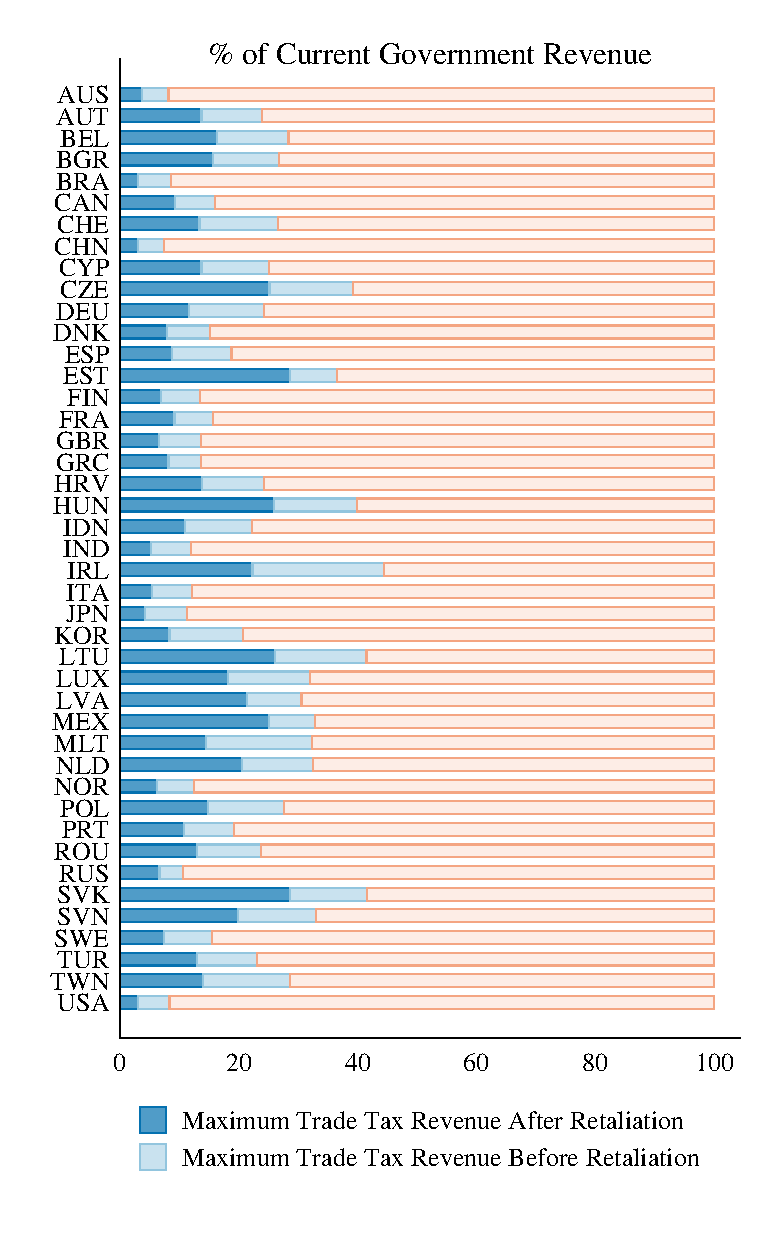
\includegraphics{Fig_J1}
\end{figure}}
\centering{
\begin{figure}[!tbh]
\caption{\label{fig: Extended Effectiveness-vs.-Efficiency}Effectiveness vs.
Efficiency Trade-Off \\ (EU members treated as autonomous taxing
authorities)}

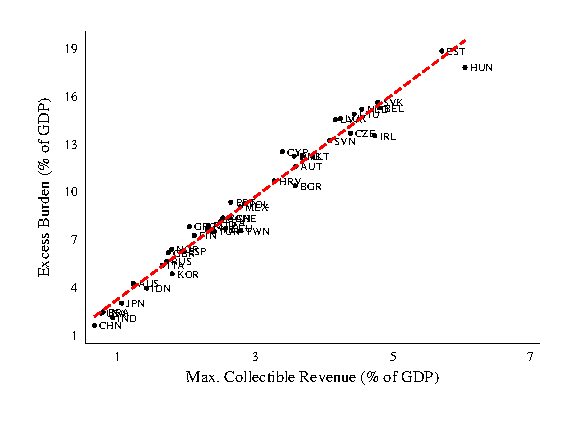
\includegraphics[scale=1.5]{Fig_J2}
\end{figure}
}
\end{document}
